\chapter{Progress}\label{progress}
\section{Writing Contributions}
\subsection{Synthetic bed topographies for Antarctica and their utility in ice sheet modelling}
I contributed to the investigation and writing of the manuscript titled ``Synthetic bed topographies for Antarctica and their utility in ice sheet modelling'', which has been submitted to the journal Proceedings of the Royal Society A. This comprehensive review and case study examines the various methods used to generate synthetic bed topographies for Antarctica, assessing their underlying objectives, associated uncertainties, and their impact on ice sheet model projections of sea level rise.
My contribution was focused on the literature review of key methodologies used to generate these topographies. I was responsible for authoring the descriptions for several prominent techniques, including:

\begin{itemize}
\item{Mass Conservation}: Detailing how this physics-informed approach, as implemented in widely-used datasets like BedMachine~\cite{Morlighem_2020} and the TELVIS algorithm~\cite{TELVIS_2011}, is used to reconstruct bed topography by ensuring the continuity of ice volume across the glacial system.
\item{Ensemble Kalman Filter (EnKF)}: Summarising this data assimilation technique which uses an ensemble of model states to estimate and update system parameters based on new observations, thereby tracking the transient evolution of an ice sheet. some relevant works include~\cite{Gillet-Chaulet_2020, Choi_2025}.
\item{Linear Perturbation Theory}: Referenced works using this method are included and discussed in section~\ref{theoretical_frameworks} of this report.
\end{itemize}

By describing these distinct approaches, their physical assumptions, and their limitations, my work helped to establish the theoretical context for the paper's case study on the Aurora Subglacial Basin. This review framed the comparison between different types of synthetic beds ("elevation-preserving" vs. "texture-preserving") and underscored how methodological choices in bed generation can significantly influence projections of future sea level contributions

\newpage
\subsection{SMUG}
I have also contributed to the investigation and writing of a manuscript detailing a new interpolation method for sparse and unevenly sampled data. The manuscript is titled: ``Antarctic bed topography estimation using a Stochastic Meshless Uncertainty Gridding (SMUG) method''. This manuscript will be submitted to Elsevier.
My contribution involved conducting a review of existing interpolation techniques helping to author the introductory section of the manuscript. My writing establishes the scientific context and rationale for the development of SMUG. I analysed several established methods used in previous Antarctic bed topography datasets, including:

\begin{itemize}
    \item{Inverse Distance Weighting (IDW)}: Used in Bedmap1~\cite{Lythe_2001}, a straightforward method that can produce overly smooth surfaces and struggle with highly variable data.

    \item{Kriging}: A geostatistical method that provides uncertainty estimates but often requires subjective, expert-driven parameter selection, which can introduce bias. This method is evaluated in Bedmap2~\cite{Fretwell_2013} and Bedmap3~\cite{Pritchard_2025} and found to produce less accurate results than other methods such as spline interpolation.

    \item{Spline Interpolation (e.g., Topogrid)}: The key technique in Bedmap2~\cite{Fretwell_2013}, this method demonstrated good performance but faced challenges in optimising smoothing parameters and honouring all data points.

    \item{Mass Conservation Methods}: Implemented in BedMachine~\cite{Morlighem_2020}, this physics-informed approach improves accuracy in data-sparse regions but requires additional datasets (like ice velocity) that are not always available.
\end{itemize}

Through my investigation, I identified and articulated key limitations and research gaps inherent in these widely-used techniques. Specifically, my writing highlighted the common difficulties in providing robust uncertainty estimates, avoiding systematic biases, and capturing the spatial correlation of errors realistically. This analysis sets the stage for the manuscript to introduce SMUG as a method designed to overcome these specific shortcomings, setting the foundation upon which the novelty and significance of the SMUG method were demonstrated in our manuscript.

\section{Recreating ISMIP-HOM}
As a first step in validating the computational framework for this project and to build a understanding foundation of the capabilities and functionality of ISSM, I replicated a series of benchmark experiments from the Ice Sheet Model Intercomparison Project for Higher-Order Models (ISMIP-HOM)~\cite{Pattyn_2008}. Successfully replicating these benchmarks demonstrates that the simulation setup is configured accurately capturing the fundamental physics of ice flow.
Part of my recreation focused on the first four diagnostic experiments (A, B, C, and D), which test a model's ability to simulate ice flow under a range of conditions. Experiments A and B involve flow over a sinusoidally varying bed topography (a "bumpy" 3D bed and a "rippled" 2D bed, respectively) with no basal sliding. These experiments are designed to evaluate the model's handling of longitudinal and vertical stress gradients induced by basal topography. Conversely, Experiments C and D feature a flat bed but introduce spatially variable basal friction, simulating the dynamics of an ice stream with slippery and sticky patches. All my models utilised full-Stokes equations (FS).
\begin{figure}[H]
    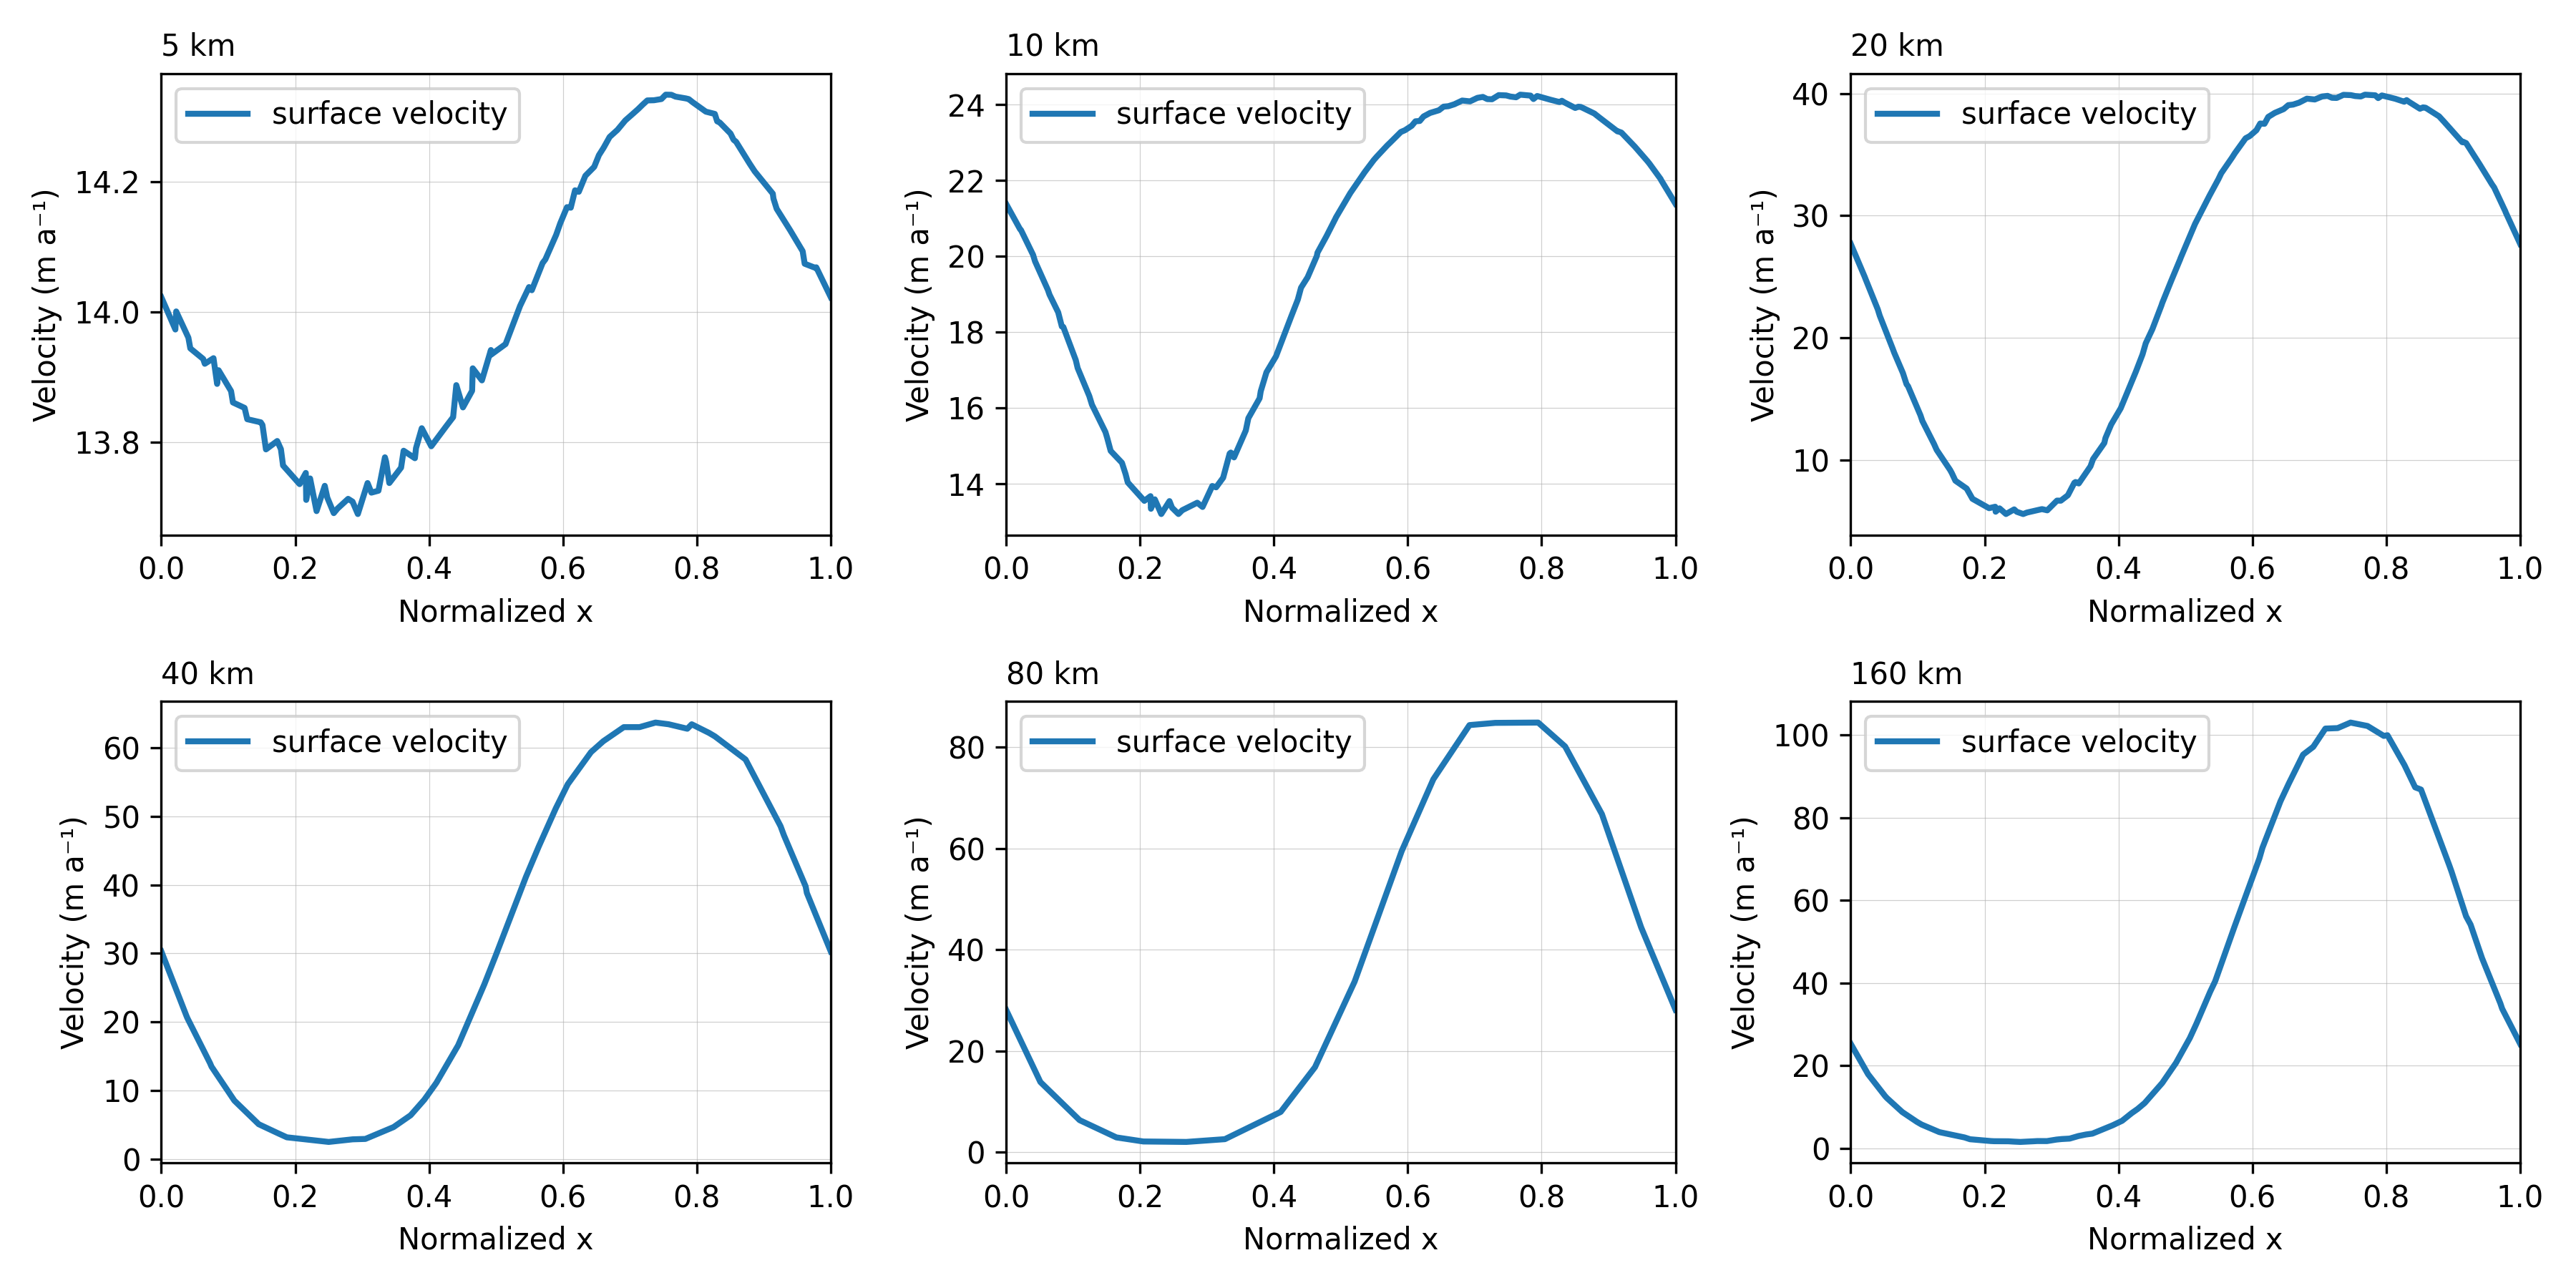
\includegraphics[scale=0.49]{figures/ExpA_velocity_panels.png}
    \caption{ISSM recreation of ISMIP-HOM Experiment A: Ice flow over a bumpy bed. The panels show the the surface velocity for a 3D ice flow simulation over a sinusoidal bed with no basal sliding ($v_b=0$). Each panel corresponds to a different domain length scale (L), from 5 km to 160 km.}
    \label{fig:4.1}
\end{figure}
\begin{figure}[H]
    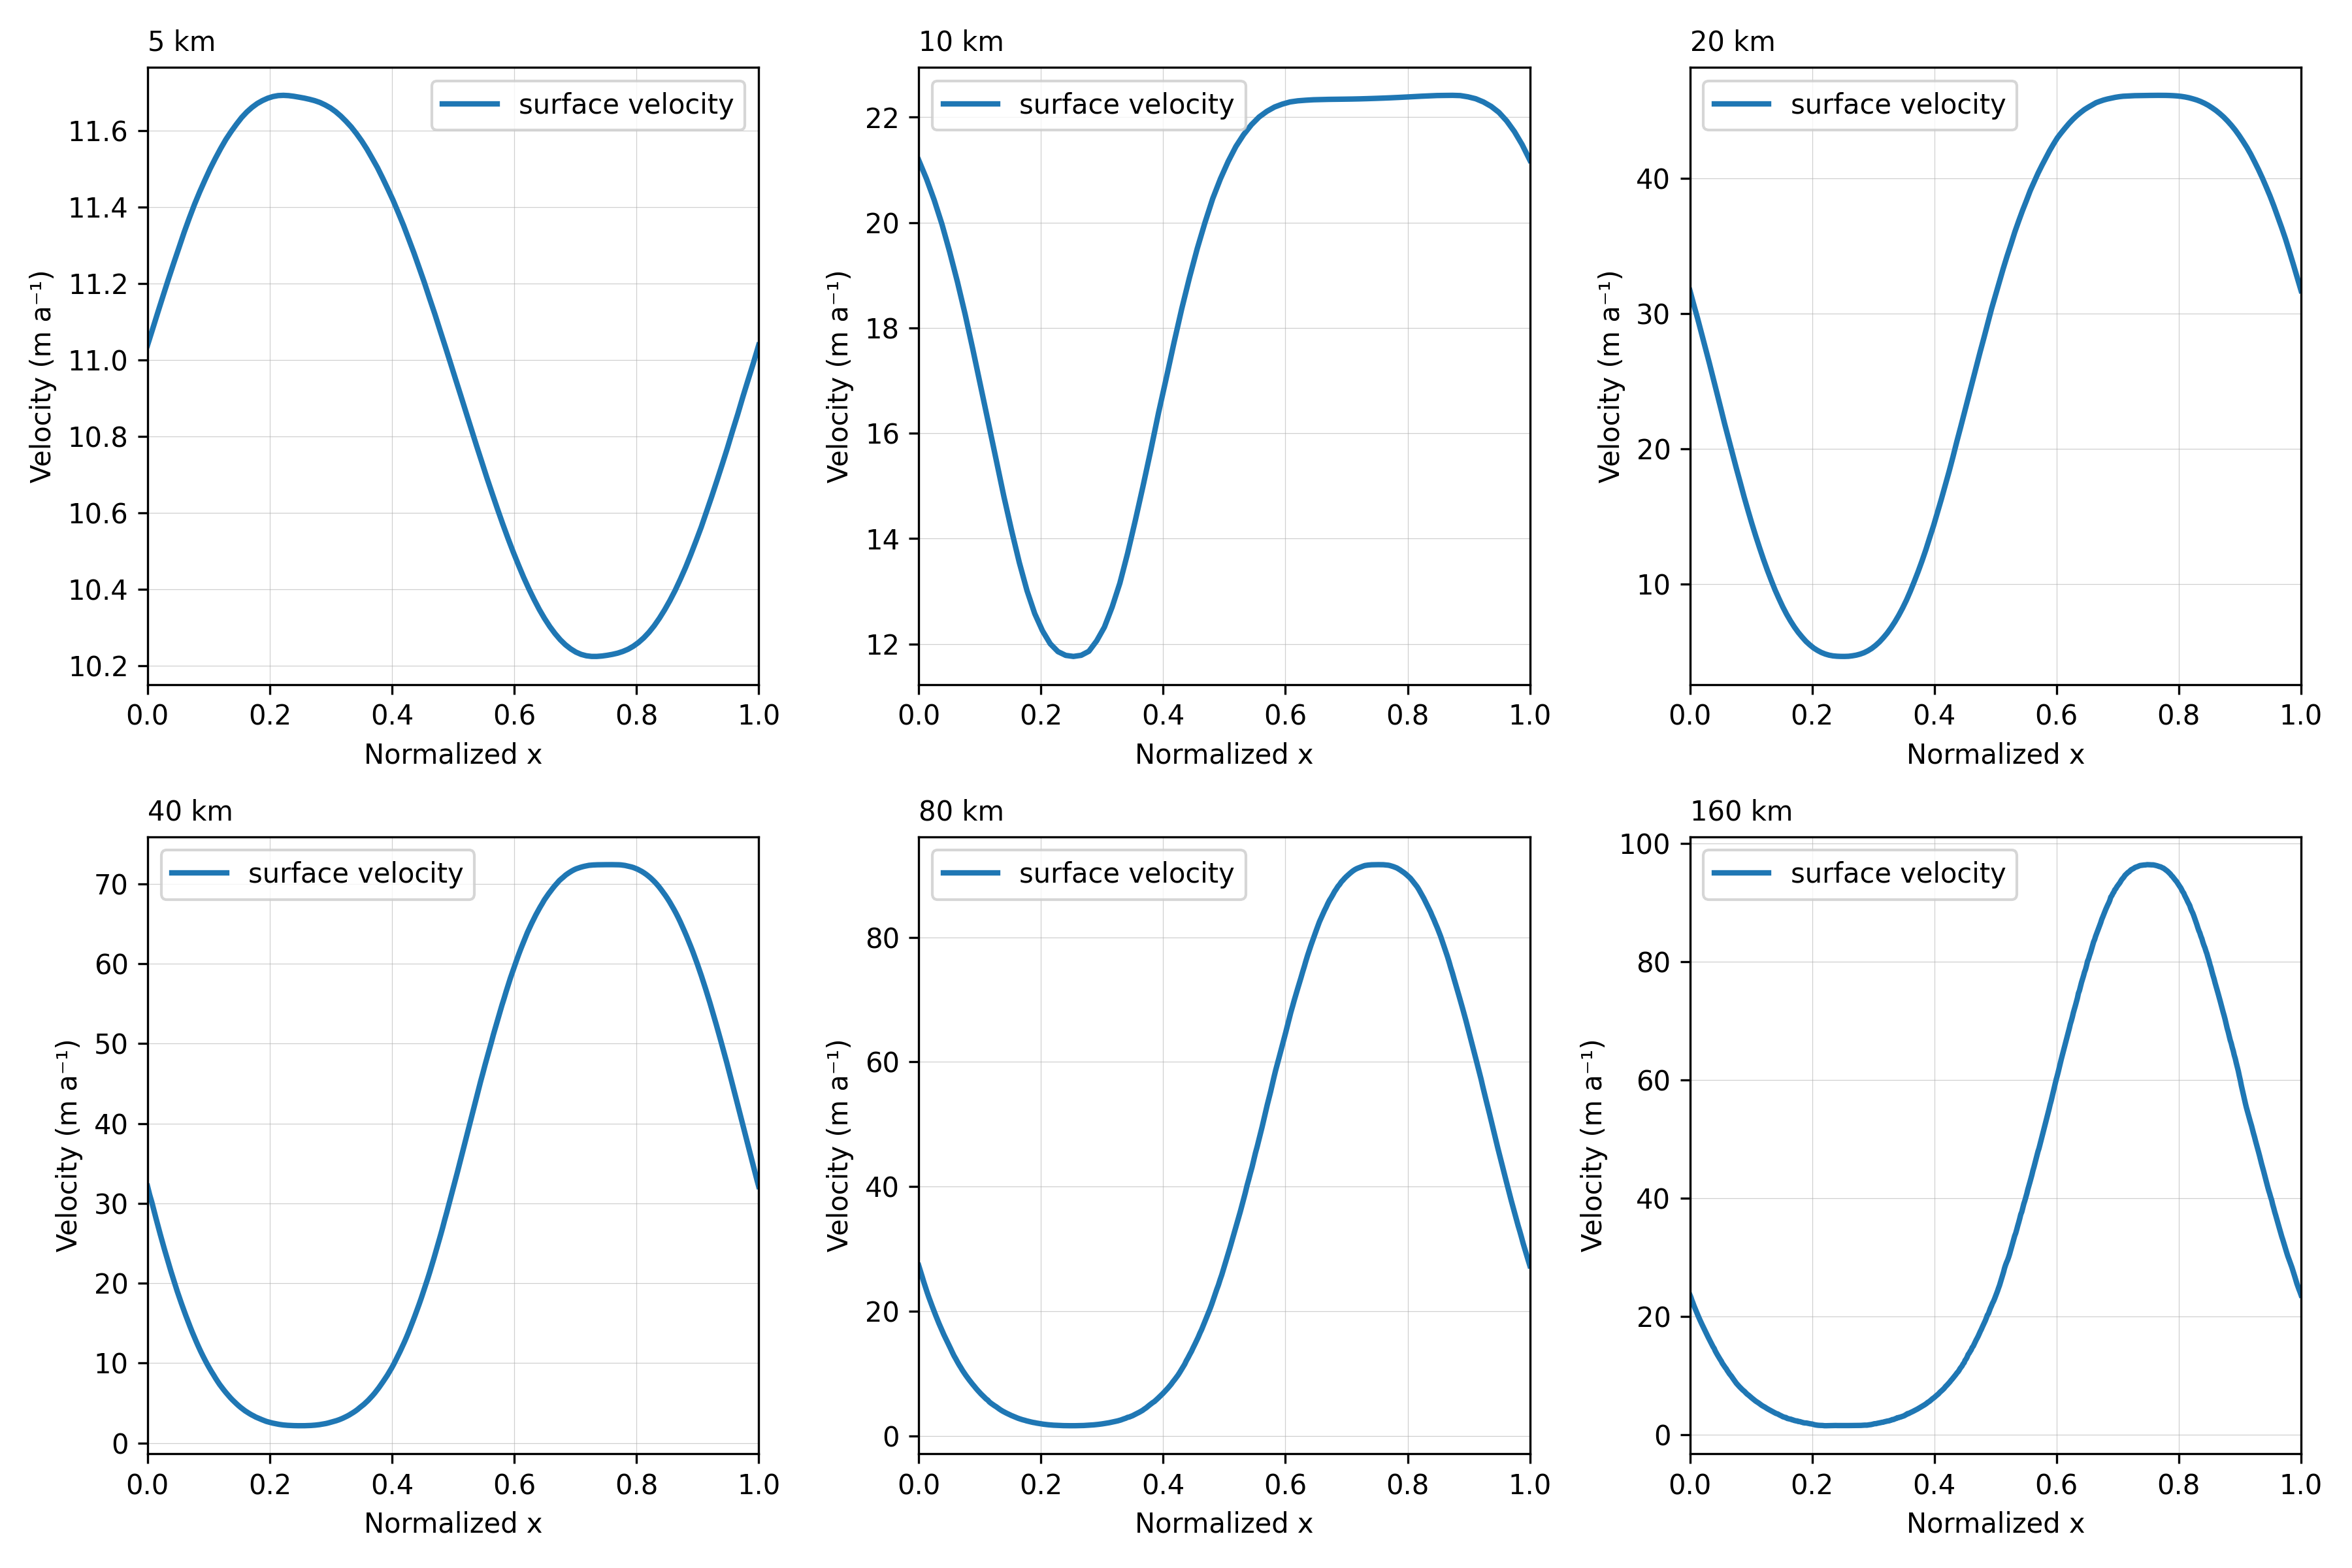
\includegraphics[scale=0.49]{figures/ExpB_velocity_panels.png}
    \caption{ISSM recreation of ISMIP-HOM Experiment B: Ice flow over a rippled bed. The panels show the surface velocity for a 2D flowline simulation. The setup is identical to Experiment A, but the basal topography does not vary in the y-direction, isolating longitudinal stress effects.}
    \label{fig:4.2}
\end{figure}
\begin{figure}[H]
    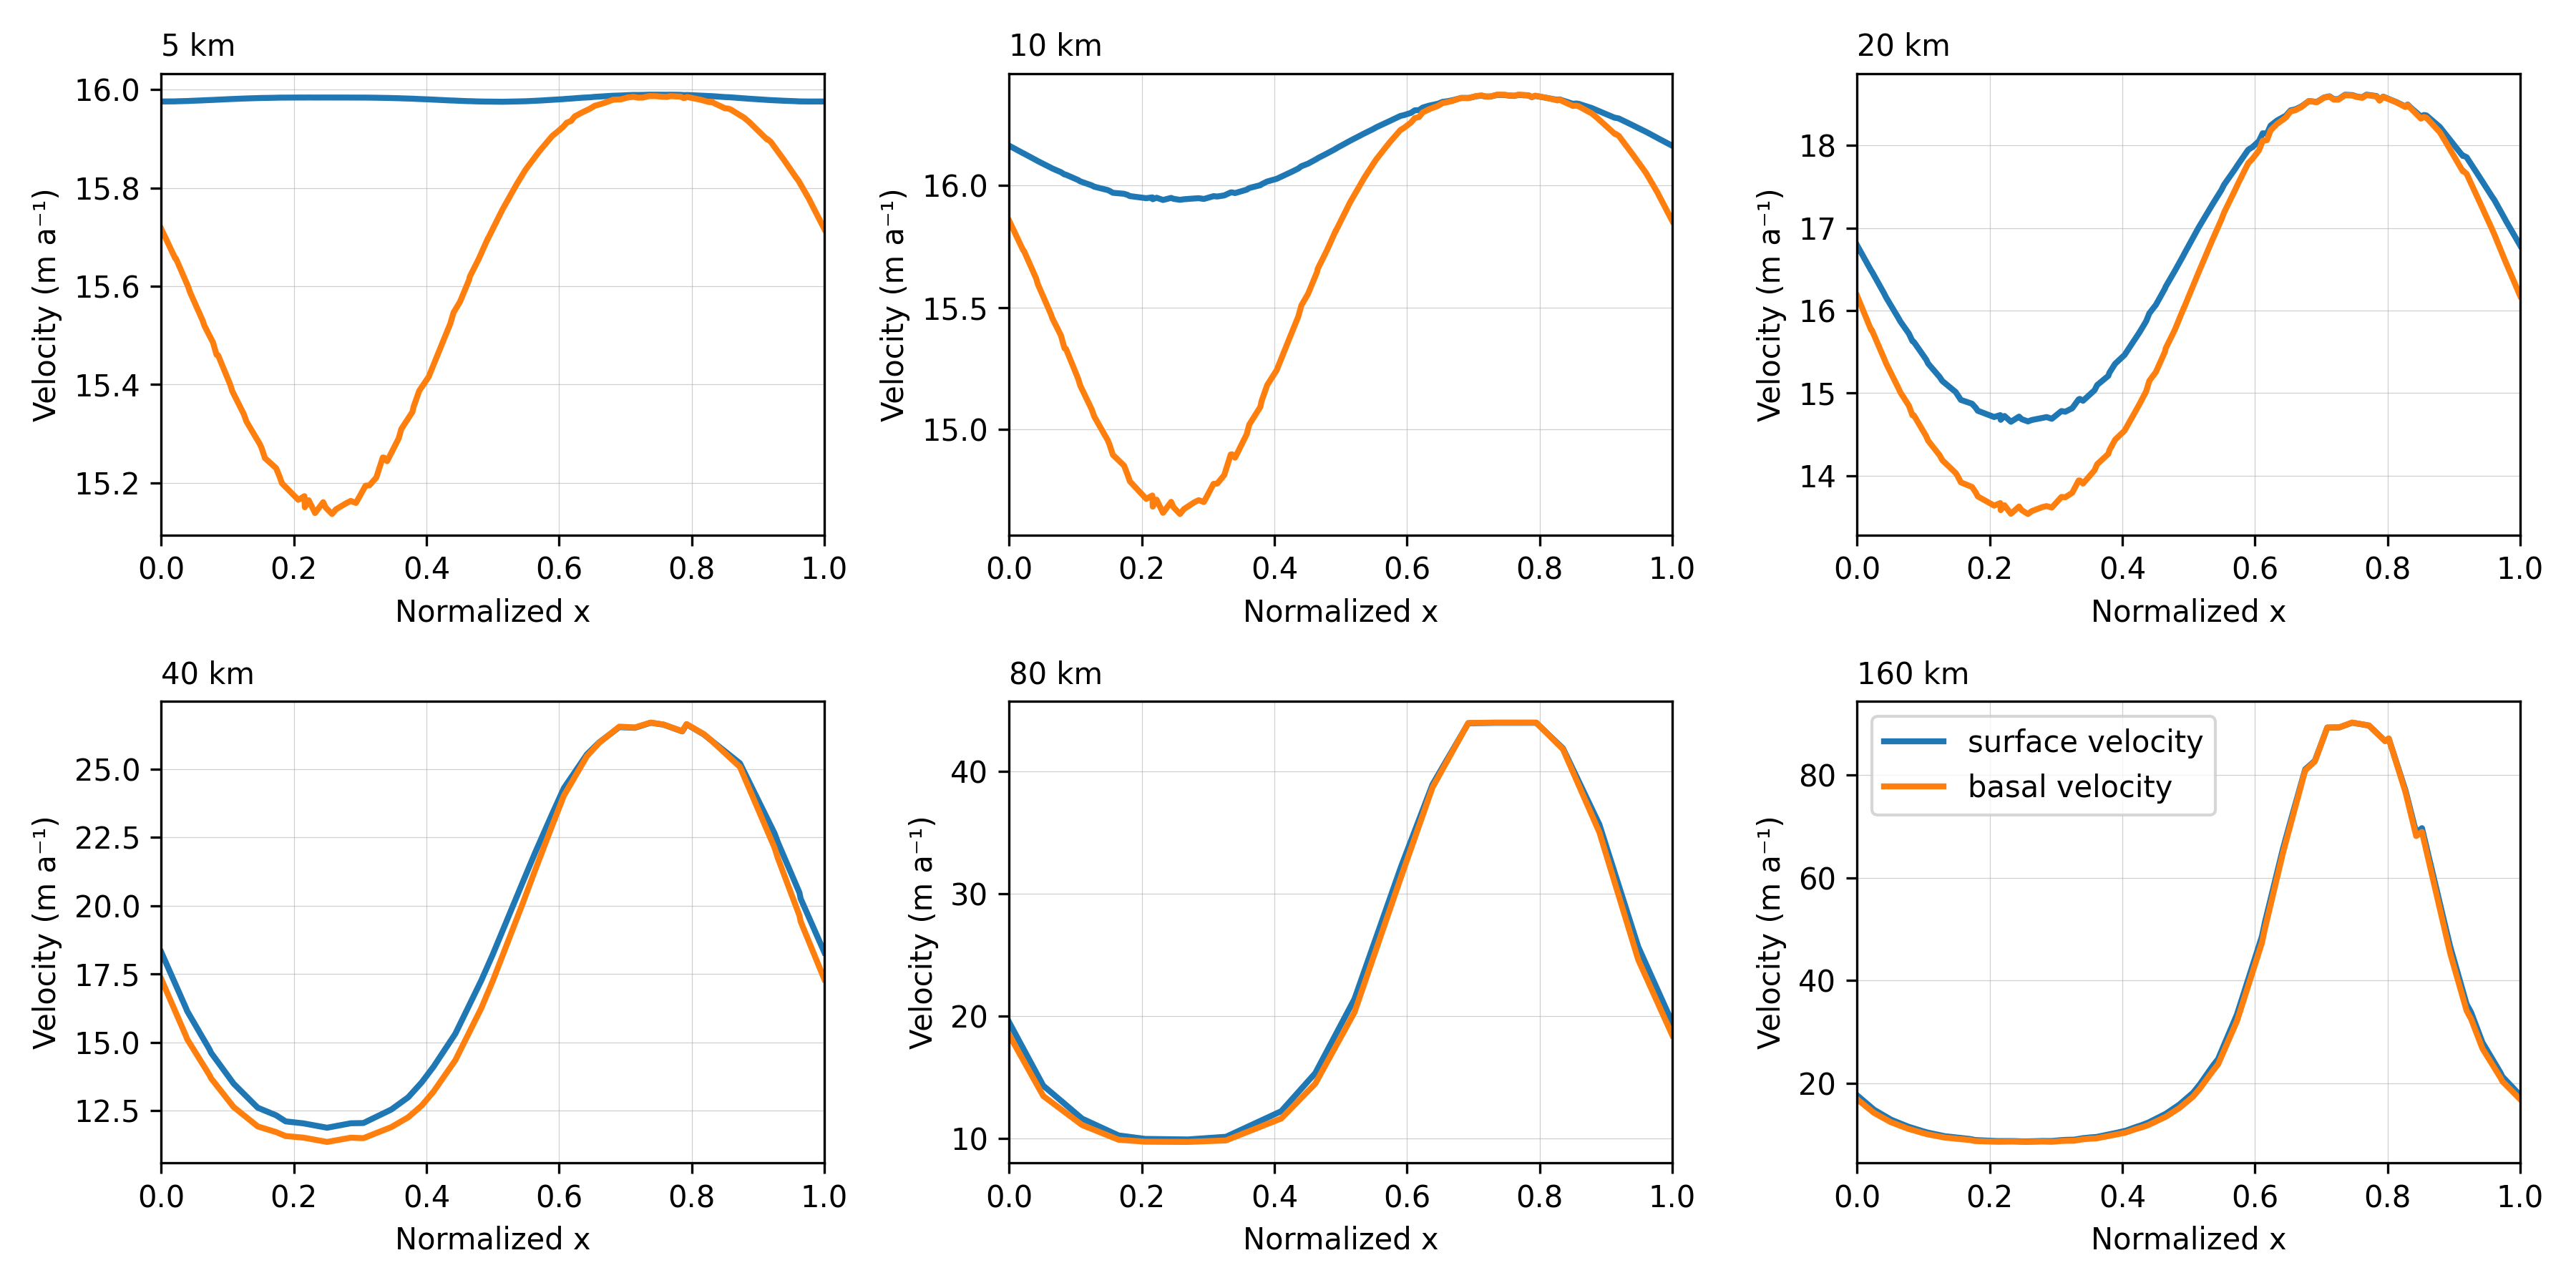
\includegraphics[scale=0.49]{figures/ExpC_velocity_panels.png}
    \caption{ISSM recreation of ISMIP-HOM Experiment C: Ice stream flow I. The panels show both surface (blue) and basal (orange) velocity for a 3D simulation over a flat bed where basal motion is governed by a spatially variable friction coefficient, $\beta^{2}(x,y)$.}
    \label{fig:4.3}
\end{figure}
\begin{figure}[H]
    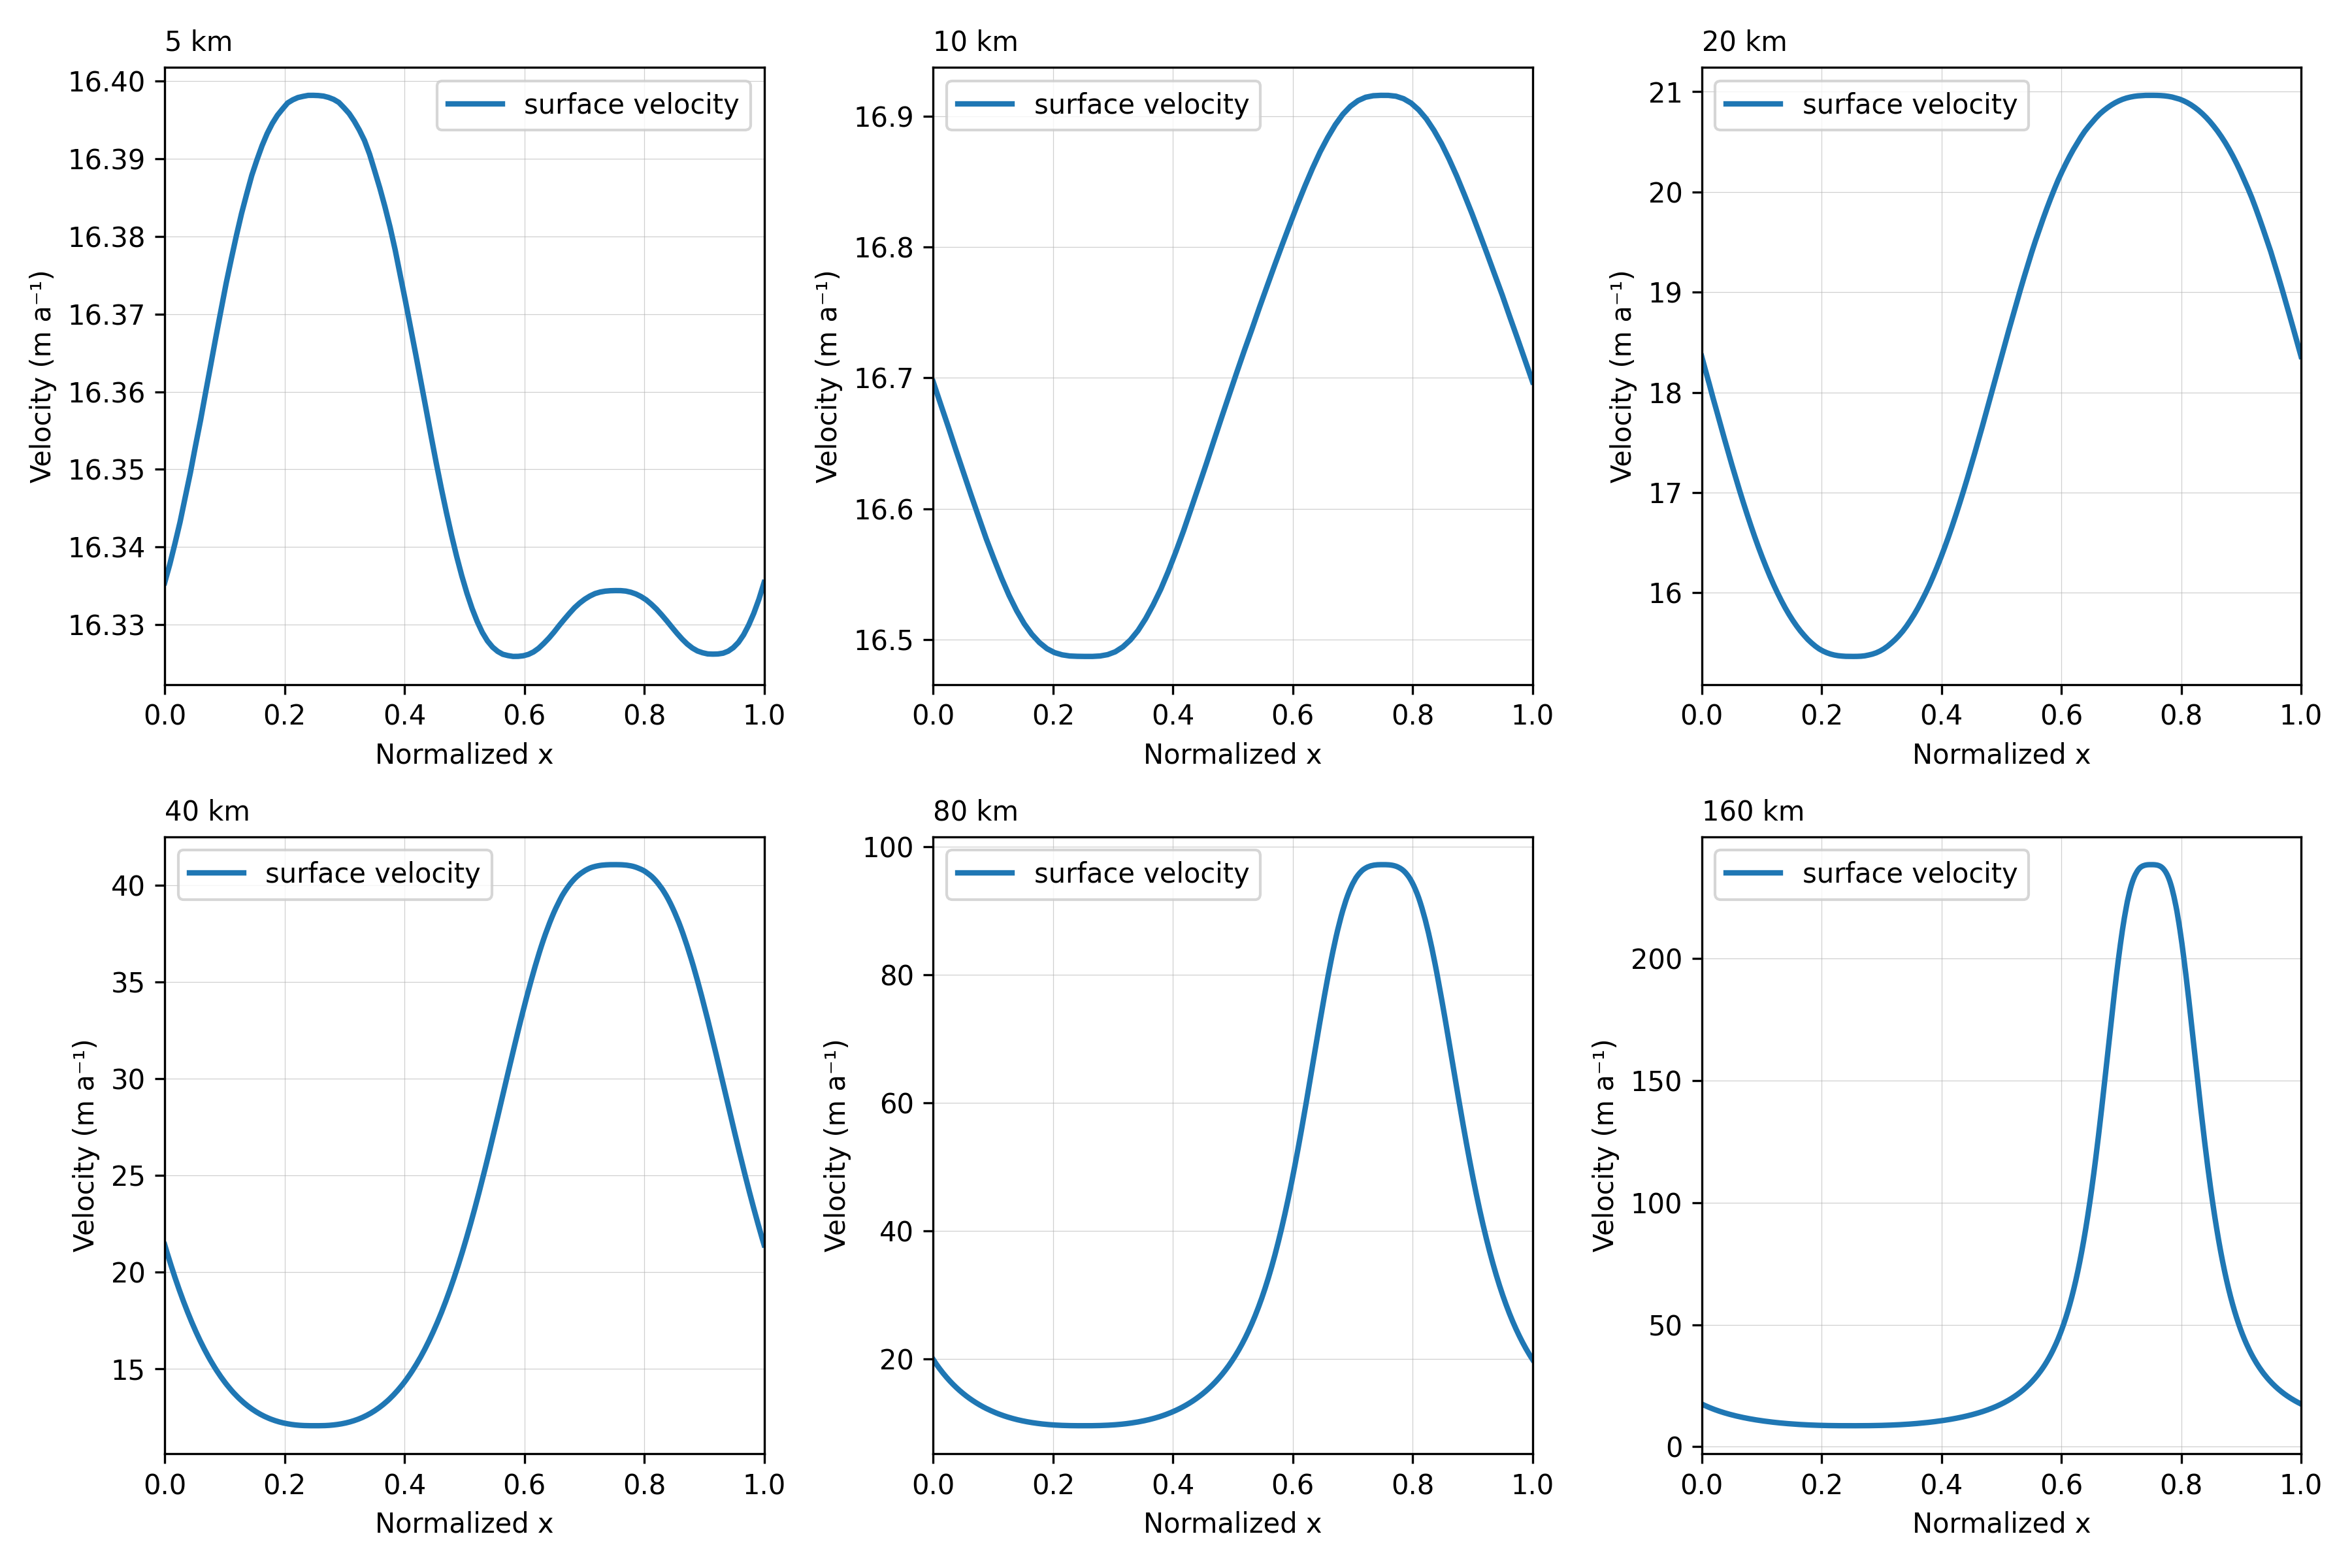
\includegraphics[scale=0.49]{figures/ExpD_velocity_panels.png}
    \caption{ ISSM recreation of ISMIP-HOM Experiment D: Ice stream flow II. The panels show the surface velocity for a 2D flowline over a flat bed with variable basal friction. The setup is identical to Experiment C, but the friction coefficient varies only in the x-direction, $\beta^{2}(x)$.}
    \label{fig:4.4}
\end{figure}

The results from these simulations demonstrate a strong agreement with the published findings in~\cite{Pattyn_2008}. For all experiments and across the different prescribed length scales \\(L = 5 km to 160 km), the calculated surface velocities closely matched the behaviour of the full-Stokes (FS) models from the original ISMIP-HOM.
My results show the same effects as the original ISMIP HOM. Smaller length scale experiments demonstrate a decreased velocity amplitude, likely due to the ice undergoing a form of viscous drag, rather than being influenced by the individual bedrock undulations. This successful validation confirms that my computational framework is robust and reliably simulates complex ice dynamics. This verification establishes a solid foundation for the application of my framework to more complex simulation settings and its subsequent research questions. In subsection~\ref{transient_ismip} I work on extending the findings in Pattyn et al, 2008. To investigate the transient (Prognostic) experiment F where the free surface is allowed to relax until a steady state is reached for zero surface mass balance~\cite{Pattyn_2008}

\subsection{Transient evolution ISMIP-HOM}\label{transient_ismip}
Building upon the diagnostic ISMIP-HOM experiments, this work extends the prognostic experiment F to systematically investigate the combined effects of rheology and basal sliding within a benchmark ice sheet model. The original experiment F included two scenarios: one with a frozen bed (no-slip) and another with linear sliding. My study expands upon these conditions by also incorporating non-linear rheology. This addition generates four distinct scenarios for comparison:
\begin{itemize}
\item{S1} No-slip (frozen) bed + Linear rheology ($n=1$).
\item{S2} No-slip (frozen) bed + Non-linear rheology ($n=3$).
\item{S3} Linear sliding + Linear rheology ($n=1$).
\item{S4} Linear sliding + Non-linear rheology ($n=3$).
\end{itemize}
While the original study by Pattyn et al. (2008) covered scenarios S1 and S3, understanding the impact of rheological assumptions is crucial for modern ice sheet modelling. During periods of rapid grounding line retreat, uncertainty in the Glen flow law exponent $n$ has been found to cause a larger spread in ice-loss projections than uncertainty in climate forcing~\cite{Getraer_2025}. Therefore, explicitly testing these different physical conditions is a critical step. This foundational analysis, validated against a well-established benchmark, will provide the necessary confidence in the modelling framework before extending the work to a suite of more complex synthetic bed topographies.
% In section~\ref{study1}, I extend these principles to investigate the transfer of more complex synthetic bed topography signals to the ice surface.

\section{Rheology and Sliding Study}\label{study1}
This study forms the core of my 'Foundational Analysis of Bed-to-Surface Signal Transfer' as outlined in Section~\ref{paper1}. The objective here is to move beyond theoretical concepts and systematically quantify how fundamental physical assumptions—specifically ice rheology and basal conditions alter the expression of subglacial topography at the ice surface. I isolate the impact of these assumptions in a controlled setup. The results from this analysis will directly inform the BedSAT framework.
Budd's sliding theory describes stress propagation through flowing ice over undulating bedrock. The stress field propagates upward at an angle, creating surface (elevation) waves that are phase-shifted by approximately $\pi/2$ relative to bedrock (elevation) features, in Budd's words: \texttt{\texttt{`the maximum shear stress occurs at the tops of the waves and the minimum in the troughs'\cite{Budd_1970}}}. 
My work up until now has been focused in building a comprehensive computational framework developed for the systematic investigation of ice dynamics. The first part of this framework is to study via flow simulations the behavior of ice to understand the relationship between basal geometry, ice rheology, and overall flow response. A key objective of this work is to understand the effect of commonly made assumptions in ice sheet modelling and their repercussions for the validity of the resulting models. This initial stage is designed to be a complete, end-to-end pipeline, from environment setup to final scientific analysis. 

\subsection{Non-Linear Rheology for Exp F}
This rheology study directly addresses a critical gap in current inversion methods. While approaches like Ockenden et al. (2023) assume linear rheology ($n=1$), my results (see Figures~\ref{fig:elev_vel_S1_S2} and~\ref{fig:elev_vel_S3_S4}) demonstrate that non-linear rheology produces substantially different bed-to-surface transfer characteristics. These findings will enable BedSAT to incorporate rheology-dependent transfer functions, potentially improving bed topography reconstruction accuracy in regions where non-linear ice behavior dominates.
In order to extend Experiment F in Pattyn et al., (2008) ISMIP-HOM to encompass non-linear rheology and still be consistent, I must ensure that different model rheologies start from identical initial conditions. The method I follow here is based on re-scaling method by Getraer and Morlighem (2025)~\cite{Getraer_2025}. Their formula ensures that the initial ice viscosity—and therefore strain rates for a given stress—is identical between simulations with different rheologies.

The fundamental model for the deformation of glacial ice and the equations which govern ice flow is Glen's flow law. 
\begin{equation}
\mathbf{\dot{\varepsilon}} \,=\, A_{n}\,\mathbf{\tau}^{n},
\end{equation}
We can also write Glen's flow law in terms of the material's resistance to deformation—the viscosity—, which is not a constant value but changes depending on stress and strain rates.
\begin{equation}
\mathbf{\tau}\,=\, 2\mu\,\mathbf{\dot{\varepsilon}},
\end{equation}
which means that $A^{-1/n} = 2\mu \mathbf{\dot{\varepsilon}}^{\frac{n-1}{n}}$, where $B=A^{-1/n}$ (Pa s$^{1/n}$) is an alternative formulation of the rate factor known as the rigidity. The rigidity parameter is commonly used in ISSM to characterise the rheology of ice in a model. This is the parameter that will be scaled.
The definition of ice viscosity uses the rigidity; for any $n$:0
\begin{equation}
\mu_n = \frac{B_n}{2\,\mathbf{\dot{\varepsilon}}^{\frac{n-1}{n}}},
\end{equation}
setting the viscosity as equal for both linear and non-linear rheology scenarios implies that the strain rates can be set as equivalent between linear and non-linear rheology scenarios
\begin{equation}
\mu_1 = \frac{B_1}{2},
\end{equation}
Then setting $\mu_1 = \mu_n$ and rearranging for $B_n$
\begin{equation}
\frac{B_1}{2} = \frac{B_n}{2\,\mathbf{\dot{\varepsilon}}^{\frac{n-1}{n}}}
\end{equation}
Letting $n = 1$, this means we are treating ice a Newtonian fluid (viscosity is independent to changes in stress). Since $B_{1}=A^{-1}$ where value of $A_{1}$ is taken as from Pattyn (2008). 
\begin{equation}
B_{1} = (2.140373×10^{-7})^{-1}\,\mathrm{Pa\,a},
\end{equation}
For the non-linear scenarios I am considering $n=4$, since the assumption of $n = 3$ for ice deformation is not universally supported and values of $n > 3$ have been inferred from real‐world glaciers. Suggesting that a value of $n=4$ better represents the actual behavior of glaciers in some places\cite{Getraer_2025}. Then scaling the rigidity for the non-linear scenarios is:
\begin{equation}
B_4 = B_1 \mathbf{\dot{\varepsilon}}^{\frac{4-1}{4}} = B_1 \mathbf{\dot{\varepsilon}}^{\frac{3}{4},}
\end{equation}
Here the strain rate is the characteristic strain rate that can be derived from the unperturbed velocity. For simple shear, $\dot{\varepsilon} \approx U / H$. Where $U$ is the mean ice velocity and $H$ is the ice thickness. 
From the grid convergence analyses in~\ref{grid_ind}, I discovered that the highest grid resolution ($2.0\times2.0$) converges to velocities $U_{\mathrm{S1}}=102.75 \, \mathrm{m\,a^{-1}}$ and $U_{\mathrm{S3}}=205.09 \, \mathrm{m\,a^{-1}}$ for the frozen and sliding scenarios respectively. The ice thickness is $H=1000~\mathrm{m}$, therefore the characteristic strain rate for S1 is $\dot{\varepsilon}_{\mathrm{S1}}=  0.10275\,\mathrm{a^{-1}}$. Leaving the scaled rigidity for the frozen bed and non-linear rheology experiment (S2) as, 
\begin{equation}
B_4 = B_1 \dot{\varepsilon}_{\mathrm{S1}}^{\frac{3}{4}}.
\end{equation}
While for S3 the characteristic strain rate is $\dot{\varepsilon}_{\mathrm{S3}}= 0.20509 \,\mathrm{a^{-1}}.$ Therefore, the scaled rigidity for the sliding and non-linear rheology experiment S4 is
\begin{equation}
B_4 = B_1 \dot{\varepsilon}_{\mathrm{S3}}^{\frac{3}{4}}.
\end{equation}
The resultant surface elevations and velocities after a 300 year transient evolution For the frozen and sliding bed scenarios are 
\begin{figure}[H]
    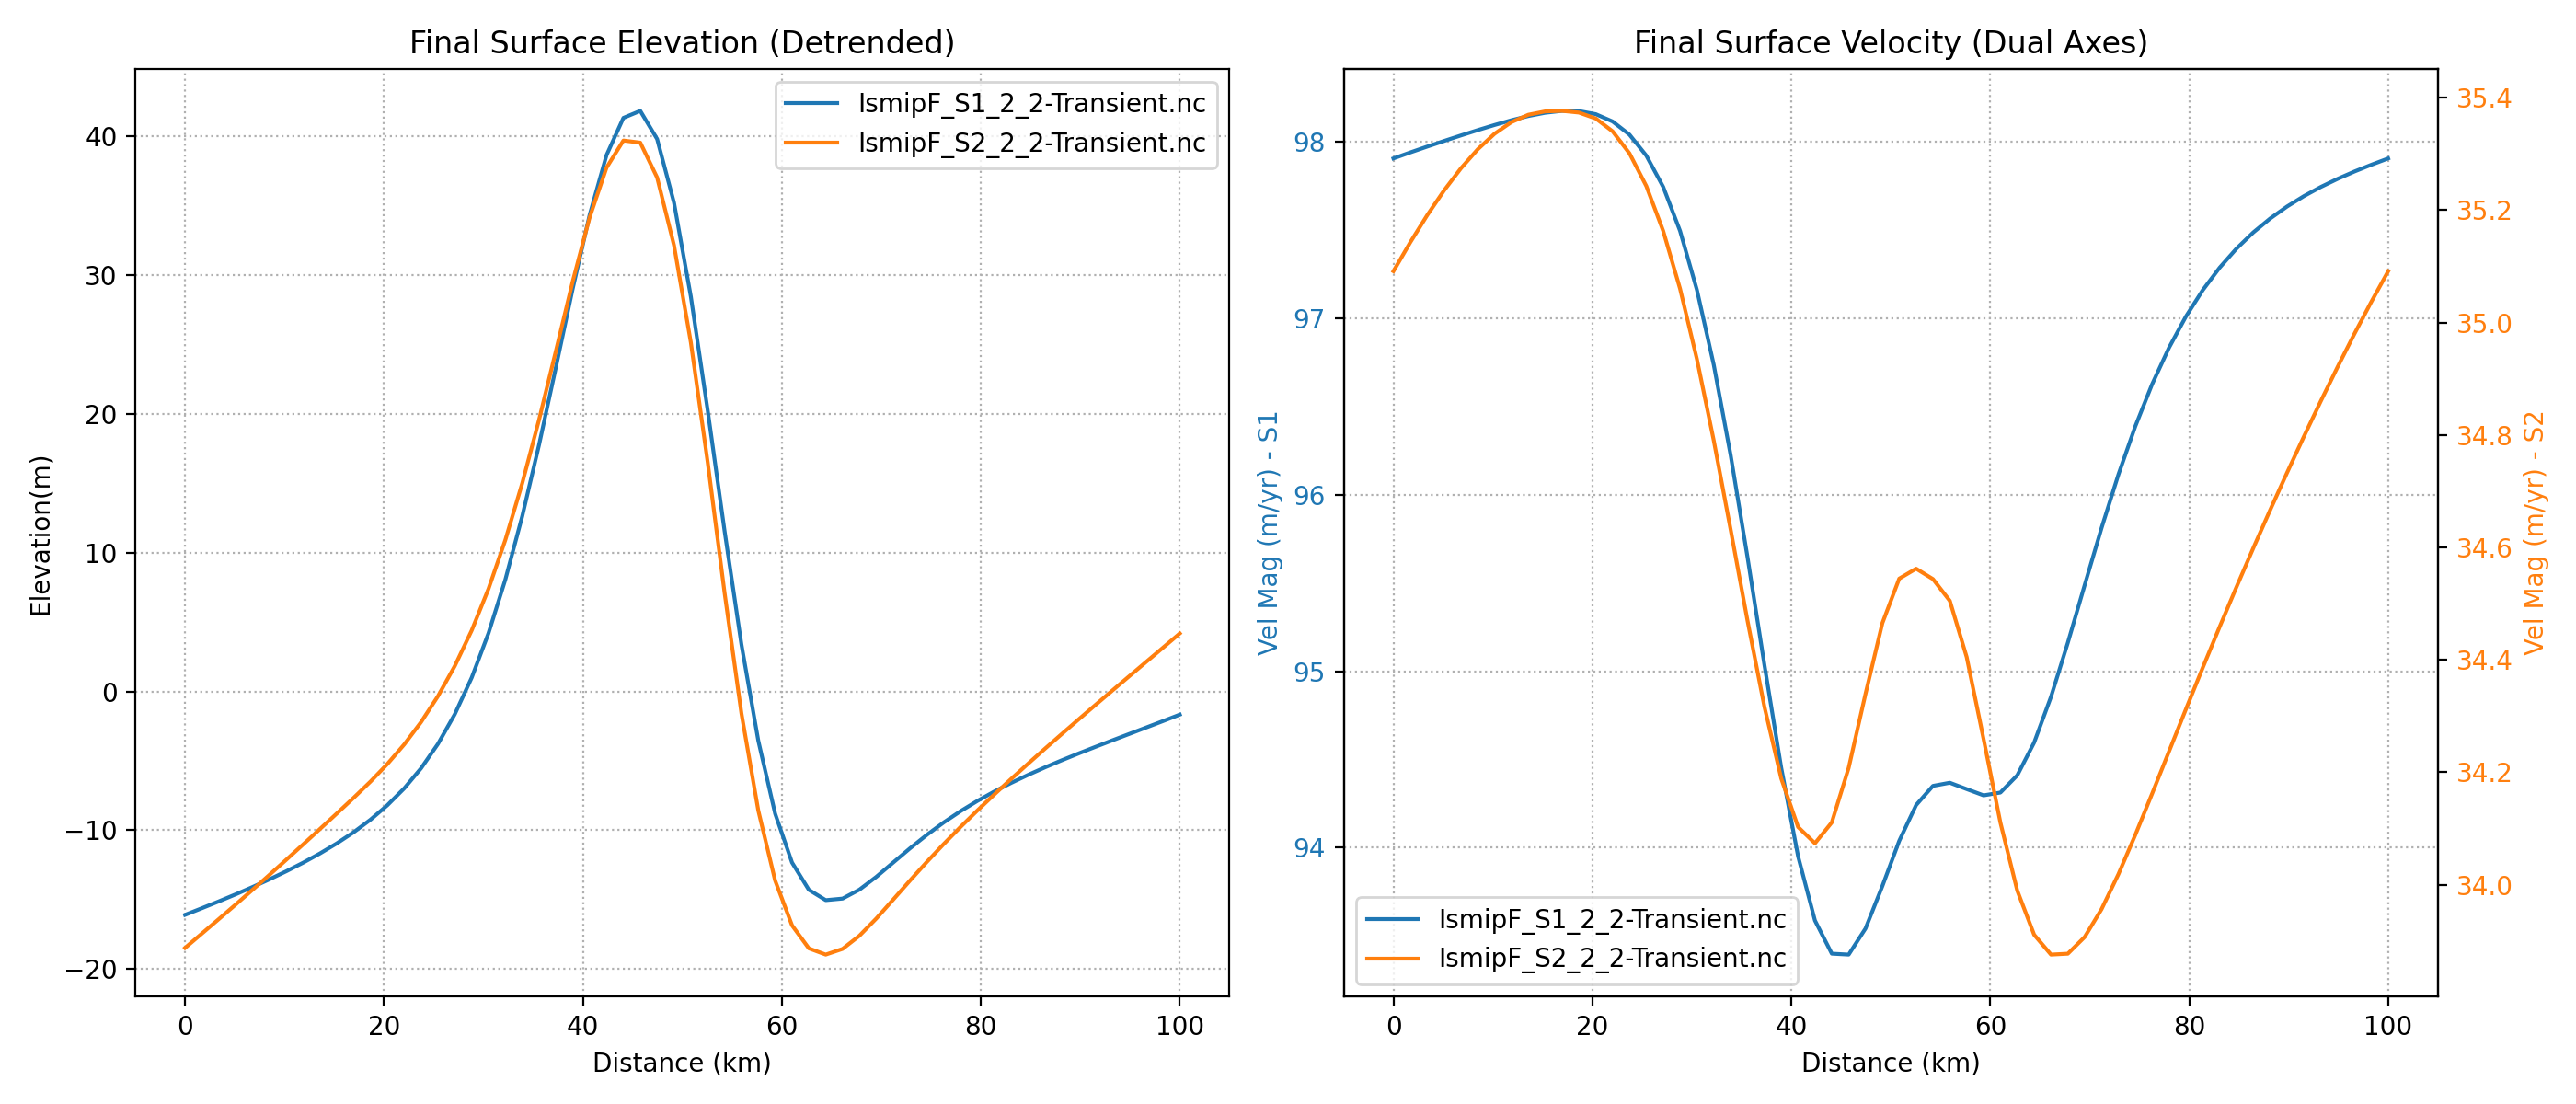
\includegraphics[scale=0.40]{figures/combined_elevation_detrended_surface_velocity_['S1']_['S2'].png}
    \caption{Final surface elevations and velocities for the original frozen bed Experiment F (S1) and the corresponding transformed to non-linear rheology experiment (S2)}
    \label{fig:elev_vel_S1_S2}
\end{figure}
\begin{figure}[H]
    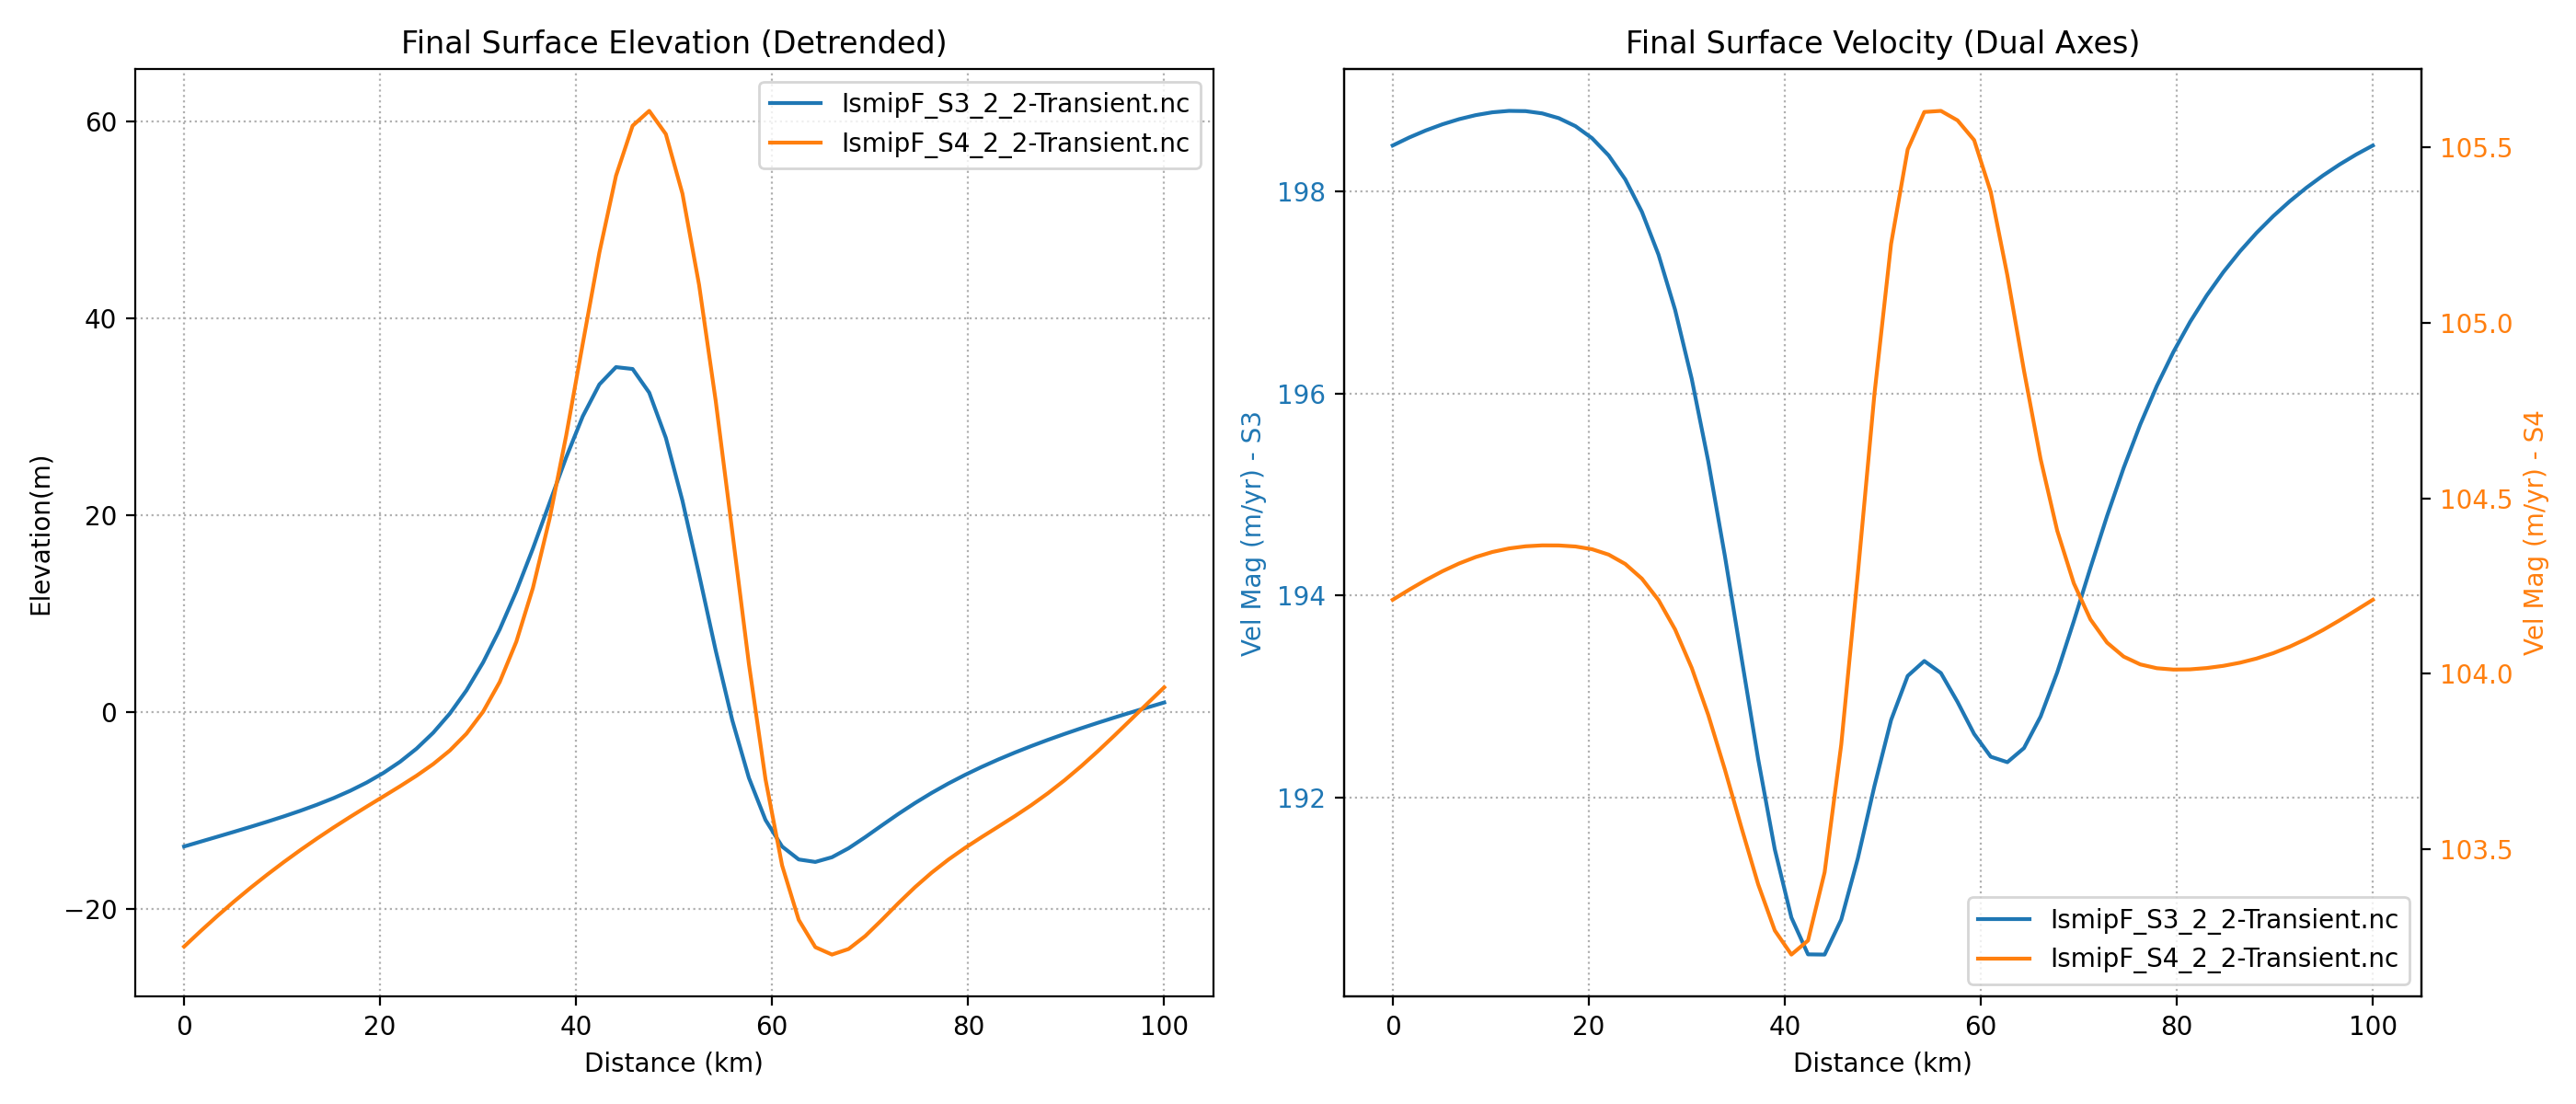
\includegraphics[scale=0.40]{figures/combined_elevation_detrended_surface_velocity_['S3']_['S4'].png}
    \caption{Final surface elevations and velocities for the original sliding bed Experiment F (S3) and the corresponding transformed to non-linear rheology experiment (S4)}
    \label{fig:elev_vel_S3_S4}
\end{figure}
These results are consistent with the surface elevation and velocities found by Pattyn et al., (2008) for Exp. F—along the central flowline of the domain—for the both the frozen and sliding experiments. The non-linear scenarios(S2 and S4) shown in orange in Figures\ref{fig:elev_vel_S3_S4} and~\ref{fig:elev_vel_S1_S2} represent the first key finding of this foundational analysis. The marked differences in both final surface elevation and velocity compared to the linear counterparts (S1, S3) provide crucial evidence for my first research question (``How does the bed topography manifest on the ice surface?''). The ice viscosity and hence its deformation is directly influenced by the stress and strain according to Glen's flow law. Given the power law relationship, using an $n = 4$ exponent leads to a strong non-linear relationship where a small increase in stress yields a much larger increase in deformation. This becomes visible as more complex flow adjustments—ice becomes softer in high stress regions and stiffer in low stress ones—in the non-linear models. These results demonstrate that the choice of rheology is not a minor parameter choice, but a control on the bed-to-surface signal transfer. It is necessary to address the nuance from these results given that while non-linear rheology better represents ice physics, this study's aim is to quantify whether this increased realism improves bed topography reconstruction accuracy enough to justify the additional computational complexity in the inversion framework. An important benefit that could come from realistic rheology assumptions in models is that they could theoretically produce surface patterns that better match satellite observations, potentially improving inversion accuracy.
The next stage in this investigation is developing a variety of synthetic bedrock topographies to understand the relationship between basal geometry, ice rheology, and overall flow response to more complex bed conditions. %This bedrock database will be used in to create a large data set of bed features to surface (response) features that can be used to train a image recognition (machine learning) model.% This model needs to be able to understand transferfunction subtleties

\newpage
\subsection{The Current Computational Framework of this Study}
This study is supported by a suite of interconnected scripts and tools designed for generating conditions, running simulations, processing output, and performing scientific analysis.
% \subsection{Synthetic Bedrock Generation}
% The \texttt{bedrock\_generator.py} script generates synthetic 1D bedrock profiles for ice flow modeling. the core functionality of this script is the creation of realistic bedrock topographies with configurable geometric properties. The bedrock profiles are defined by the following four key parameters that can be varied systematically:
% \begin{itemize}
% \item{Amplitude} Controls the vertical scale of undulations (e.g., 19.2 m to 38.4 m).
% \item{Wavelength} Controls the horizontal scale of undulations (e.g., 3.84 km to 19.2 km).
% \item{Skewness} Controls the asymmetry of the undulations.
% \item{Kurtosis} Controls the peakedness or flatness of the features.
% \end{itemize}

% The generated profiles are saved to \texttt{.npz} files and are loaded by the ice flow simulation script to ensure consistent and reproducible experimental setups.

% \begin{figure}[H]
%     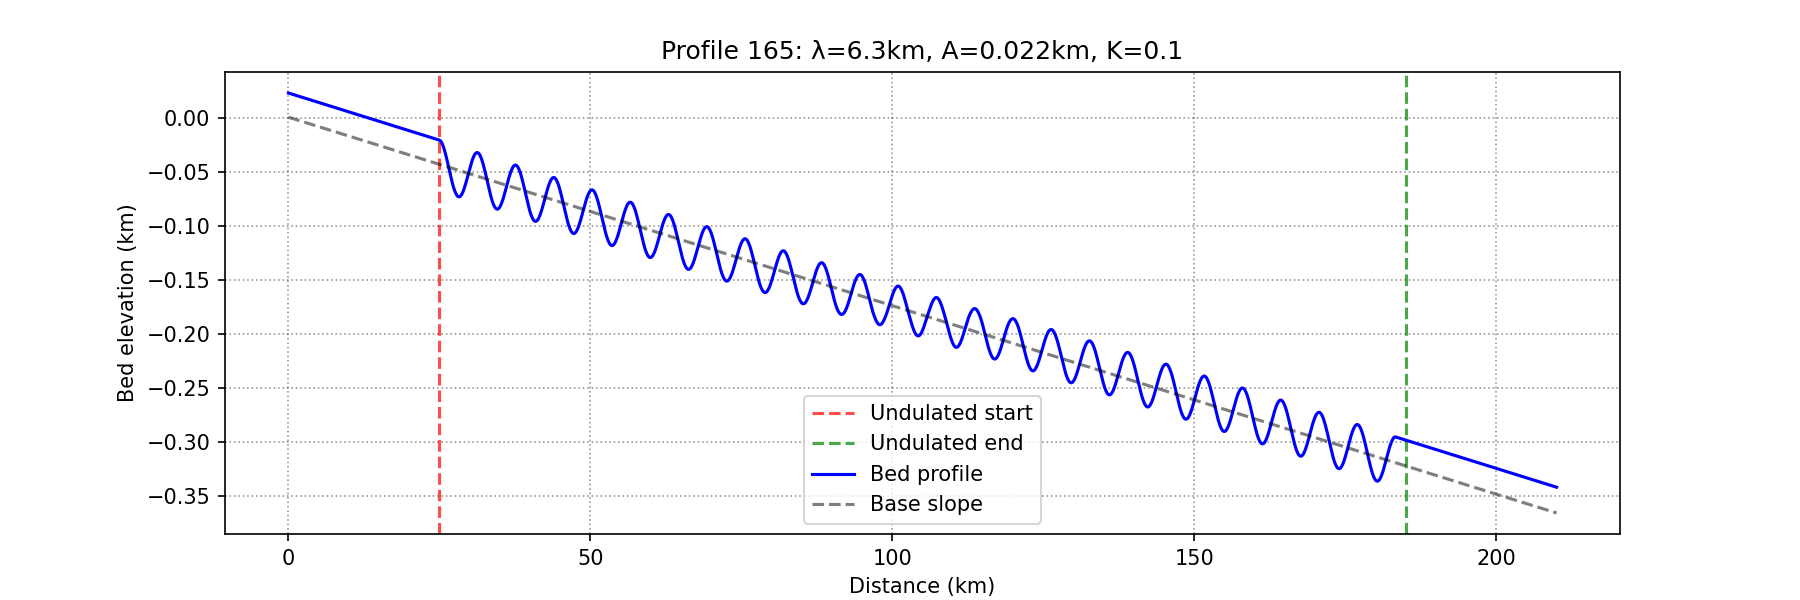
\includegraphics[scale=0.45]{figures/bedrock_profile_165.png}
%     \caption{Database sample: Profile 165 has perturbation wavelength $\lambda=6.336$~km, amplitude $0.022$~km, kurtosis $K=0.1$}
%     \label{fig:}
% \end{figure}
% % def analyse_driving_stress(md, L):
% The domain length for all bedrock profiles is $210$~km with $100$~m horizontal resolution, however the undulated (perturbation) region is $160$~km in length leaving $25$~km flattened areas in the outer regions of the bedrock are there to minimise large driving stress differences between boundaries (something that can be particularly problematic for simulating non-linear rheology scenarios), they also ensure physically consistent periodicity for the numerical simulation.
\subsection{Ice Flow Simulation}
The core of this study is a time evolution flow simulation of fully grounded ice over 300 years with daily time steps. This simulation is designed to systematically investigate the relationship between basal geometry, ice rheology and flow response by running a series of ISMIP-HOM style experiments~\cite{Pattyn_2008} that can later be analysed in detail with other data processing tools~\ref{dataviz}. The simulations solve Higher order (HO) ice flow equations for a static diagnostic stress balance and a transient run (which includes stress balance and mass transport configurations).
The simulation utilises periodic boundary conditions which represents a section of an infinitely long ice sheet effectively eliminating edge effects that would arise from standard inlet/outlet boundaries. The script couples the inlet and outlet velocities by matching vertices in the base layer and then extruding this setup vertically. This ensures that the ice flow is continuous and that the dynamics are driven solely by the underlying topography and internal stresses, which is crucial for studying the transfer of bedrock signals to the surface.
This approach has proved to be highly successful, yielding stable and physically realistic velocities across experimental scenarios. The results are consistent with established benchmarks like ISMIP-HOM and show the expected physical relationships (e.g., faster flow with sliding and non-linear rheology).
The experimental design tests different physical conditions being built around four benchmark experiments from subsection~\ref{transient_ismip}.  
The simulation friction parameters are identical to those set in Pattyn et al., (2008) which themselves follow the scaling given by Gudmundsson (2003), where the basal friction coefficient is related to the slip ratio $c$ by
\begin{equation}
\beta^2 = \left (c A H\right )^{-1}
\end{equation}
Where S1, S2 utilise a frozen bed condition ($c = 0$) while S3, S4 utilise a sliding bed ($c = 1$).
The main simulation scripts produce~\texttt{.nc} files and binary \texttt{.outbin} files for full simulation results (when run locally and on the NCI Gadi system respectively).
The simulation framework in this study includes capabilities for systematic grid convergence testing, comparing solutions across multiple mesh resolutions to ensure the results are independent of the mesh discretisation, (see Section~\ref{grid_ind}).
\newpage
\subsection{Data Processing and Visualization Tools}\label{dataviz}
I have developed a set of robust, high-performance scripts to handle the large volume of data produced by the ice flow simulations. (Note that: All batch scripts have their individual file processing counterpart)
\begin{figure}[H]
    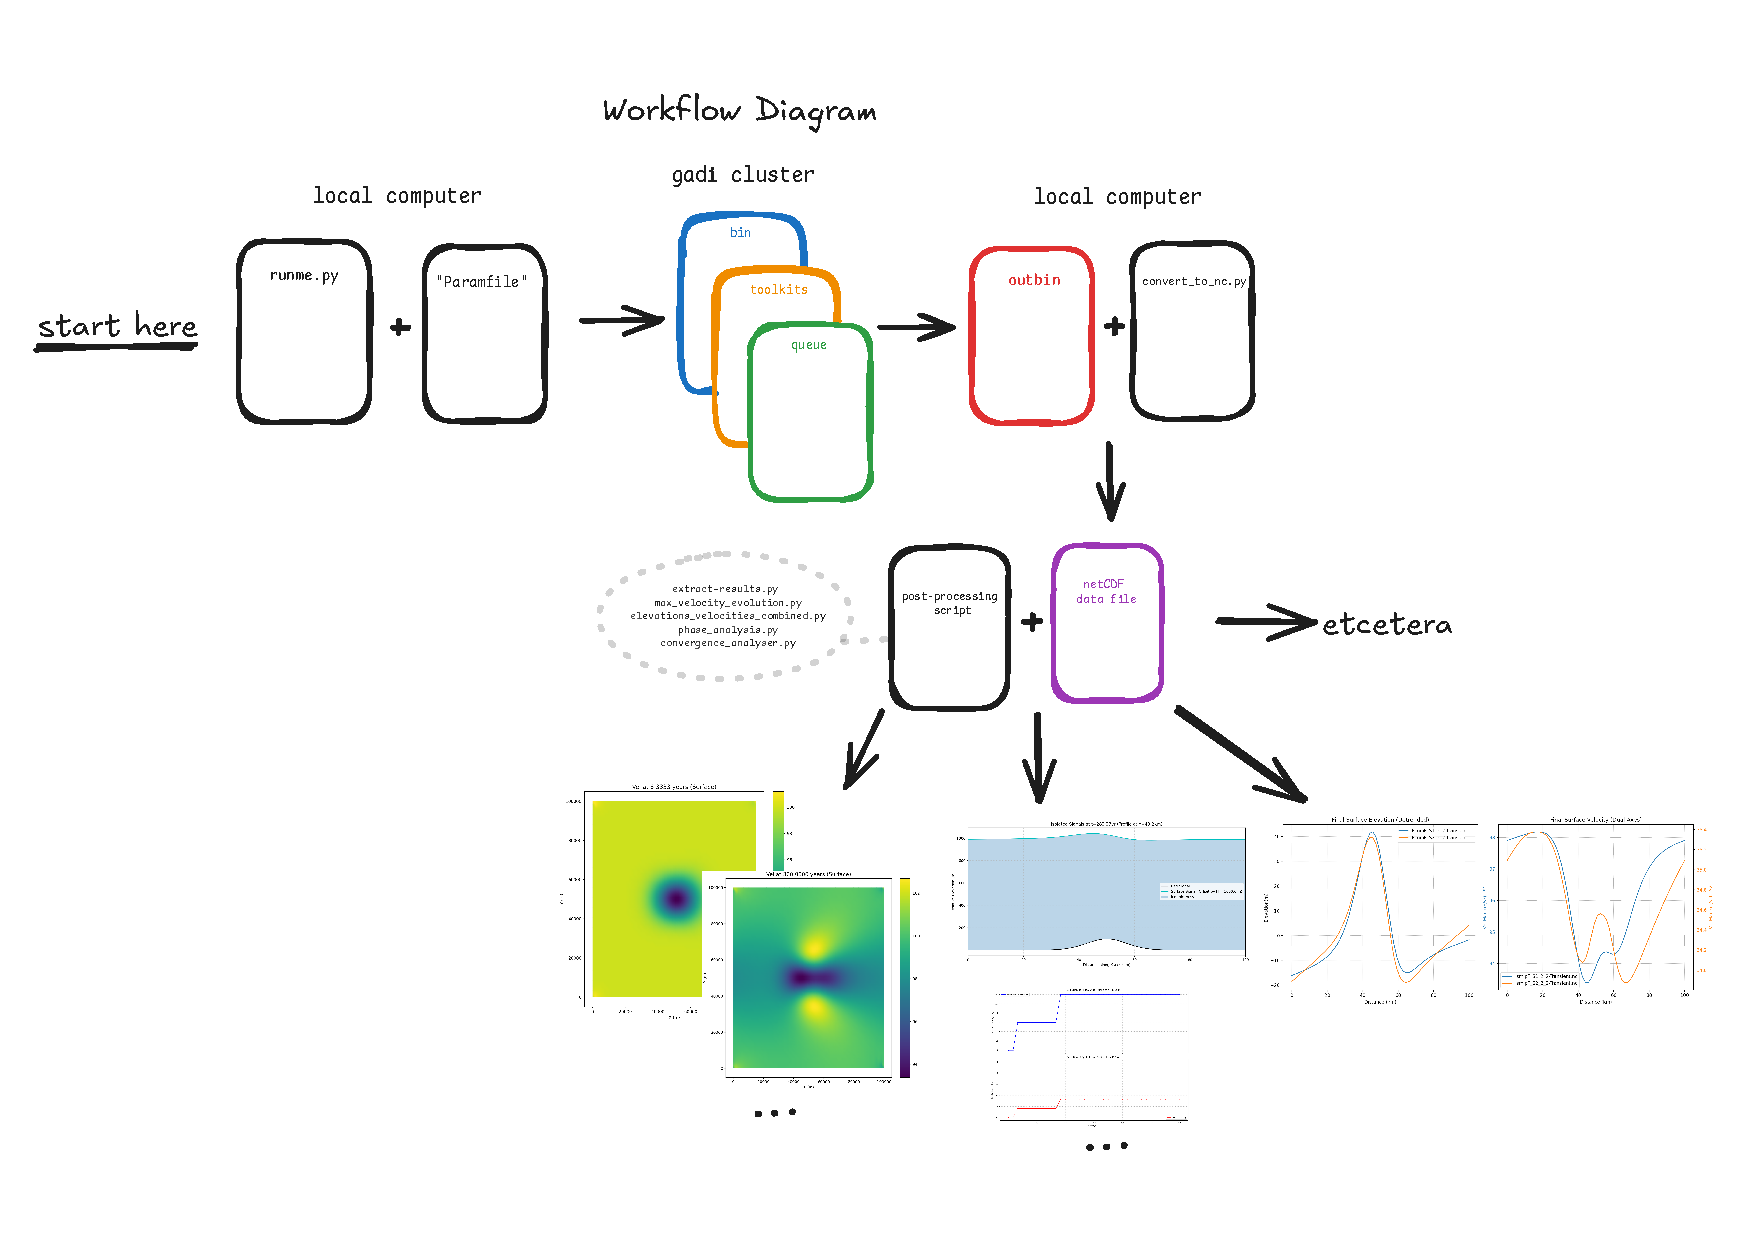
\includegraphics[scale=0.58]{figures/workflow_diagram.pdf}
    \caption{Diagrammatic representation of the current workflow using my ice simulation and analysis suite. For a particular simulation I will extract the results and visually inspect the output using  all analysis scripts in the suite.}
    \label{fig:workflow}
\end{figure}
\begin{enumerate}
\item{Binary to NetCDF Conversion} A batch-capable tool (\texttt{batch\_convert.py}) converts ISSM \texttt{.outbin} files into the standard, portable NetCDF format. This script supports parallel processing for high throughput.
\item{Result Extraction and Visualization} A batch script (\texttt{batch\_extract\_results.py}) that automatically finds and processes NetCDF files to generate visualisations of key fields like velocity and pressure. 
\item{Targeted Scientific Plotting} Additional scripts are used to create specific scientific plots.
\end{enumerate}
As per Figure~\ref{fig:workflow}, my workflow requires more automation. I still need to develop tools to do most of the post processing analysis in the cluster. This is  a work in progress.

\subsection{Scientific Analysis Tools} 
\subsubsection{Grid Independence}\label{grid_ind}
In order to  perform quantitative analysis on the simulation results. I developed a convergence analysis script: \texttt{convergence\_analyser.py}.
Grid convergence analysis is a fundamental verification technique in computational modeling that ensures numerical solutions are approaching the true solution as mesh resolution increases. The key principle is that as the grid is refined (smaller elements, more nodes), the numerical error should decrease systematically.
The grid analysis involved running simulations across 16 distinct mesh resolutions, generated by independently varying both the horizontal (H) and vertical (V) grid densities. Note that I have kept the vertical layer thickness constant. I applied resolution scaling factors of $2.0$ i.e. double the resolution, $0.5$ i.e. half the mesh resolution, $1.0$ i.e. no scaling and $1.5$ i.e. 50\% scaling. I designated the solution from the highest resolution mesh, corresponding to scaling factors of ($H=2.0, V=2.0$) as the reference solution against which all coarser meshes were compared. Refined meshes (either horizontal or vertical) often require smaller time steps to satisfy the Courant-Friedrichs-Lewy (CFL) condition and maintain solver stability. To satisfy this criterion I scaled the time step for each simulation matching the largest resolution factor independently if it was horizontal or vertical scaling.
The primary metric of this script is the L2 relative error, a global, scale-dependent measure that quantifies the overall difference between two solutions. In my analysis, I chose a convergence threshold of $1\%$—since estimates of other uncertainties are expected to be larger than grid errors—when comparing the solutions to the baseline. If the L2 norm of the data is very close to zero (less than $10^{-6}$), the analysis reports the absolute error to avoid division by a tiny, unstable number. Otherwise, it calculates and reports the standard relative error as a percentage.
The \texttt{convergence\_analyser.py} script generates a standardised $2\times2$ plot (see figures~\ref{fig:grid_conv_S1},~\ref{fig:grid_conv_S2},~\ref{fig:grid_conv_S3},~\ref{fig:grid_conv_S4}) to provide a comprehensive view of convergence via L2 error bars, and the maximum velocity at every time step. In addition the output plot shows visual velocity comparisons along a centre line in the y dimension. This is done for surface and basal velocities for each mesh resolution tested. The code identifies all unique y-coordinates present in the mesh layer (surface or base) then finds the y-coordinate that is numerically closest (given some threshold) to the defined geometric centre line, then it selects all nodes whose y-coordinate matches this identified ``closest'' y-coordinate. The script effectively extracts the entire mesh line closest to the ideal centre for each simulation. The code also establishes a reference grid based on the baseline resolution chosen, then sorts and interpolates the velocity data based on this reference grid iteratively for all resolutions, the script interpolates the sorted velocity data for each resolution onto the common reference grid. 
\begin{figure}[H]
    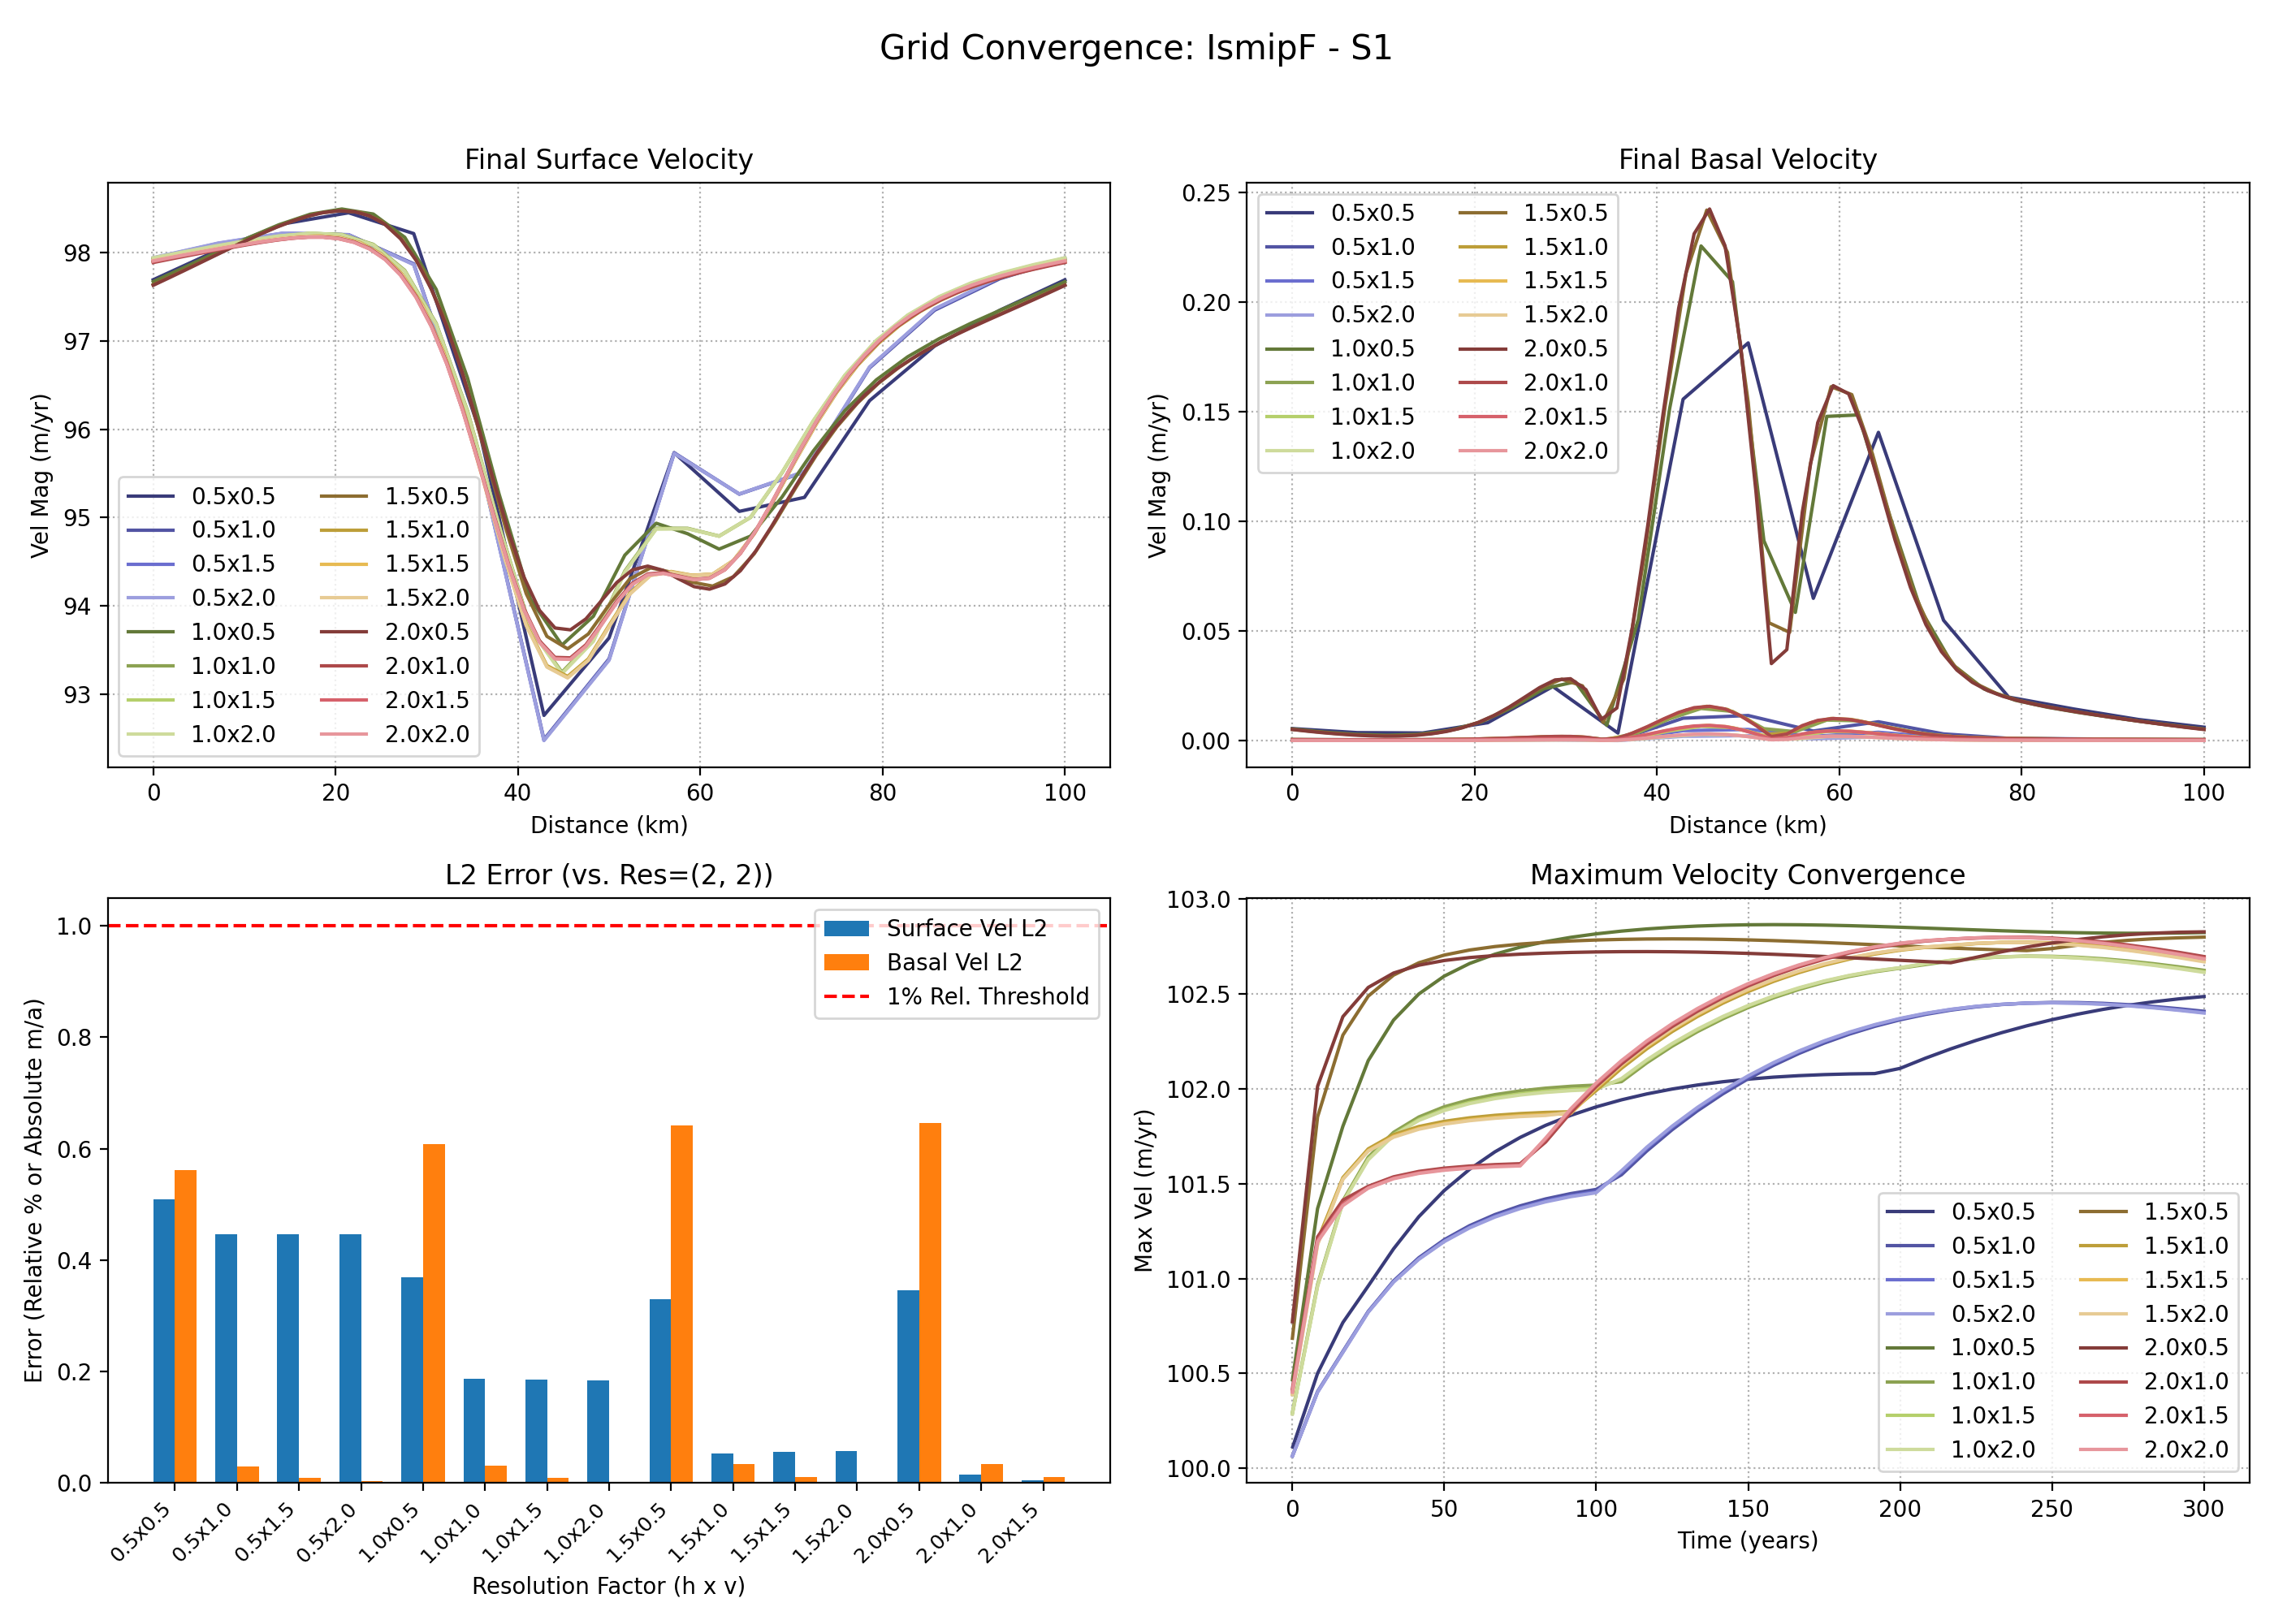
\includegraphics[scale=0.40]{figures/IsmipF_S1_convergence_summary.png}
    \caption{Grid convergence analysis for Scenario S1 (frozen bed, linear rheology, $n=1$). The four panels show: (top-left) final surface velocity profiles and (top-right) final basal velocity profiles for 16 different mesh resolutions; (bottom-left) the L2 relative error of each simulation compared to the highest-resolution mesh ($2.0\times2.0$), with a 1\% relative error threshold indicated by the dashed line; and (bottom-right) the evolution of the maximum velocity over the 300-year simulation period}
    \label{fig:grid_conv_S1}
\end{figure}
\begin{figure}[H]
    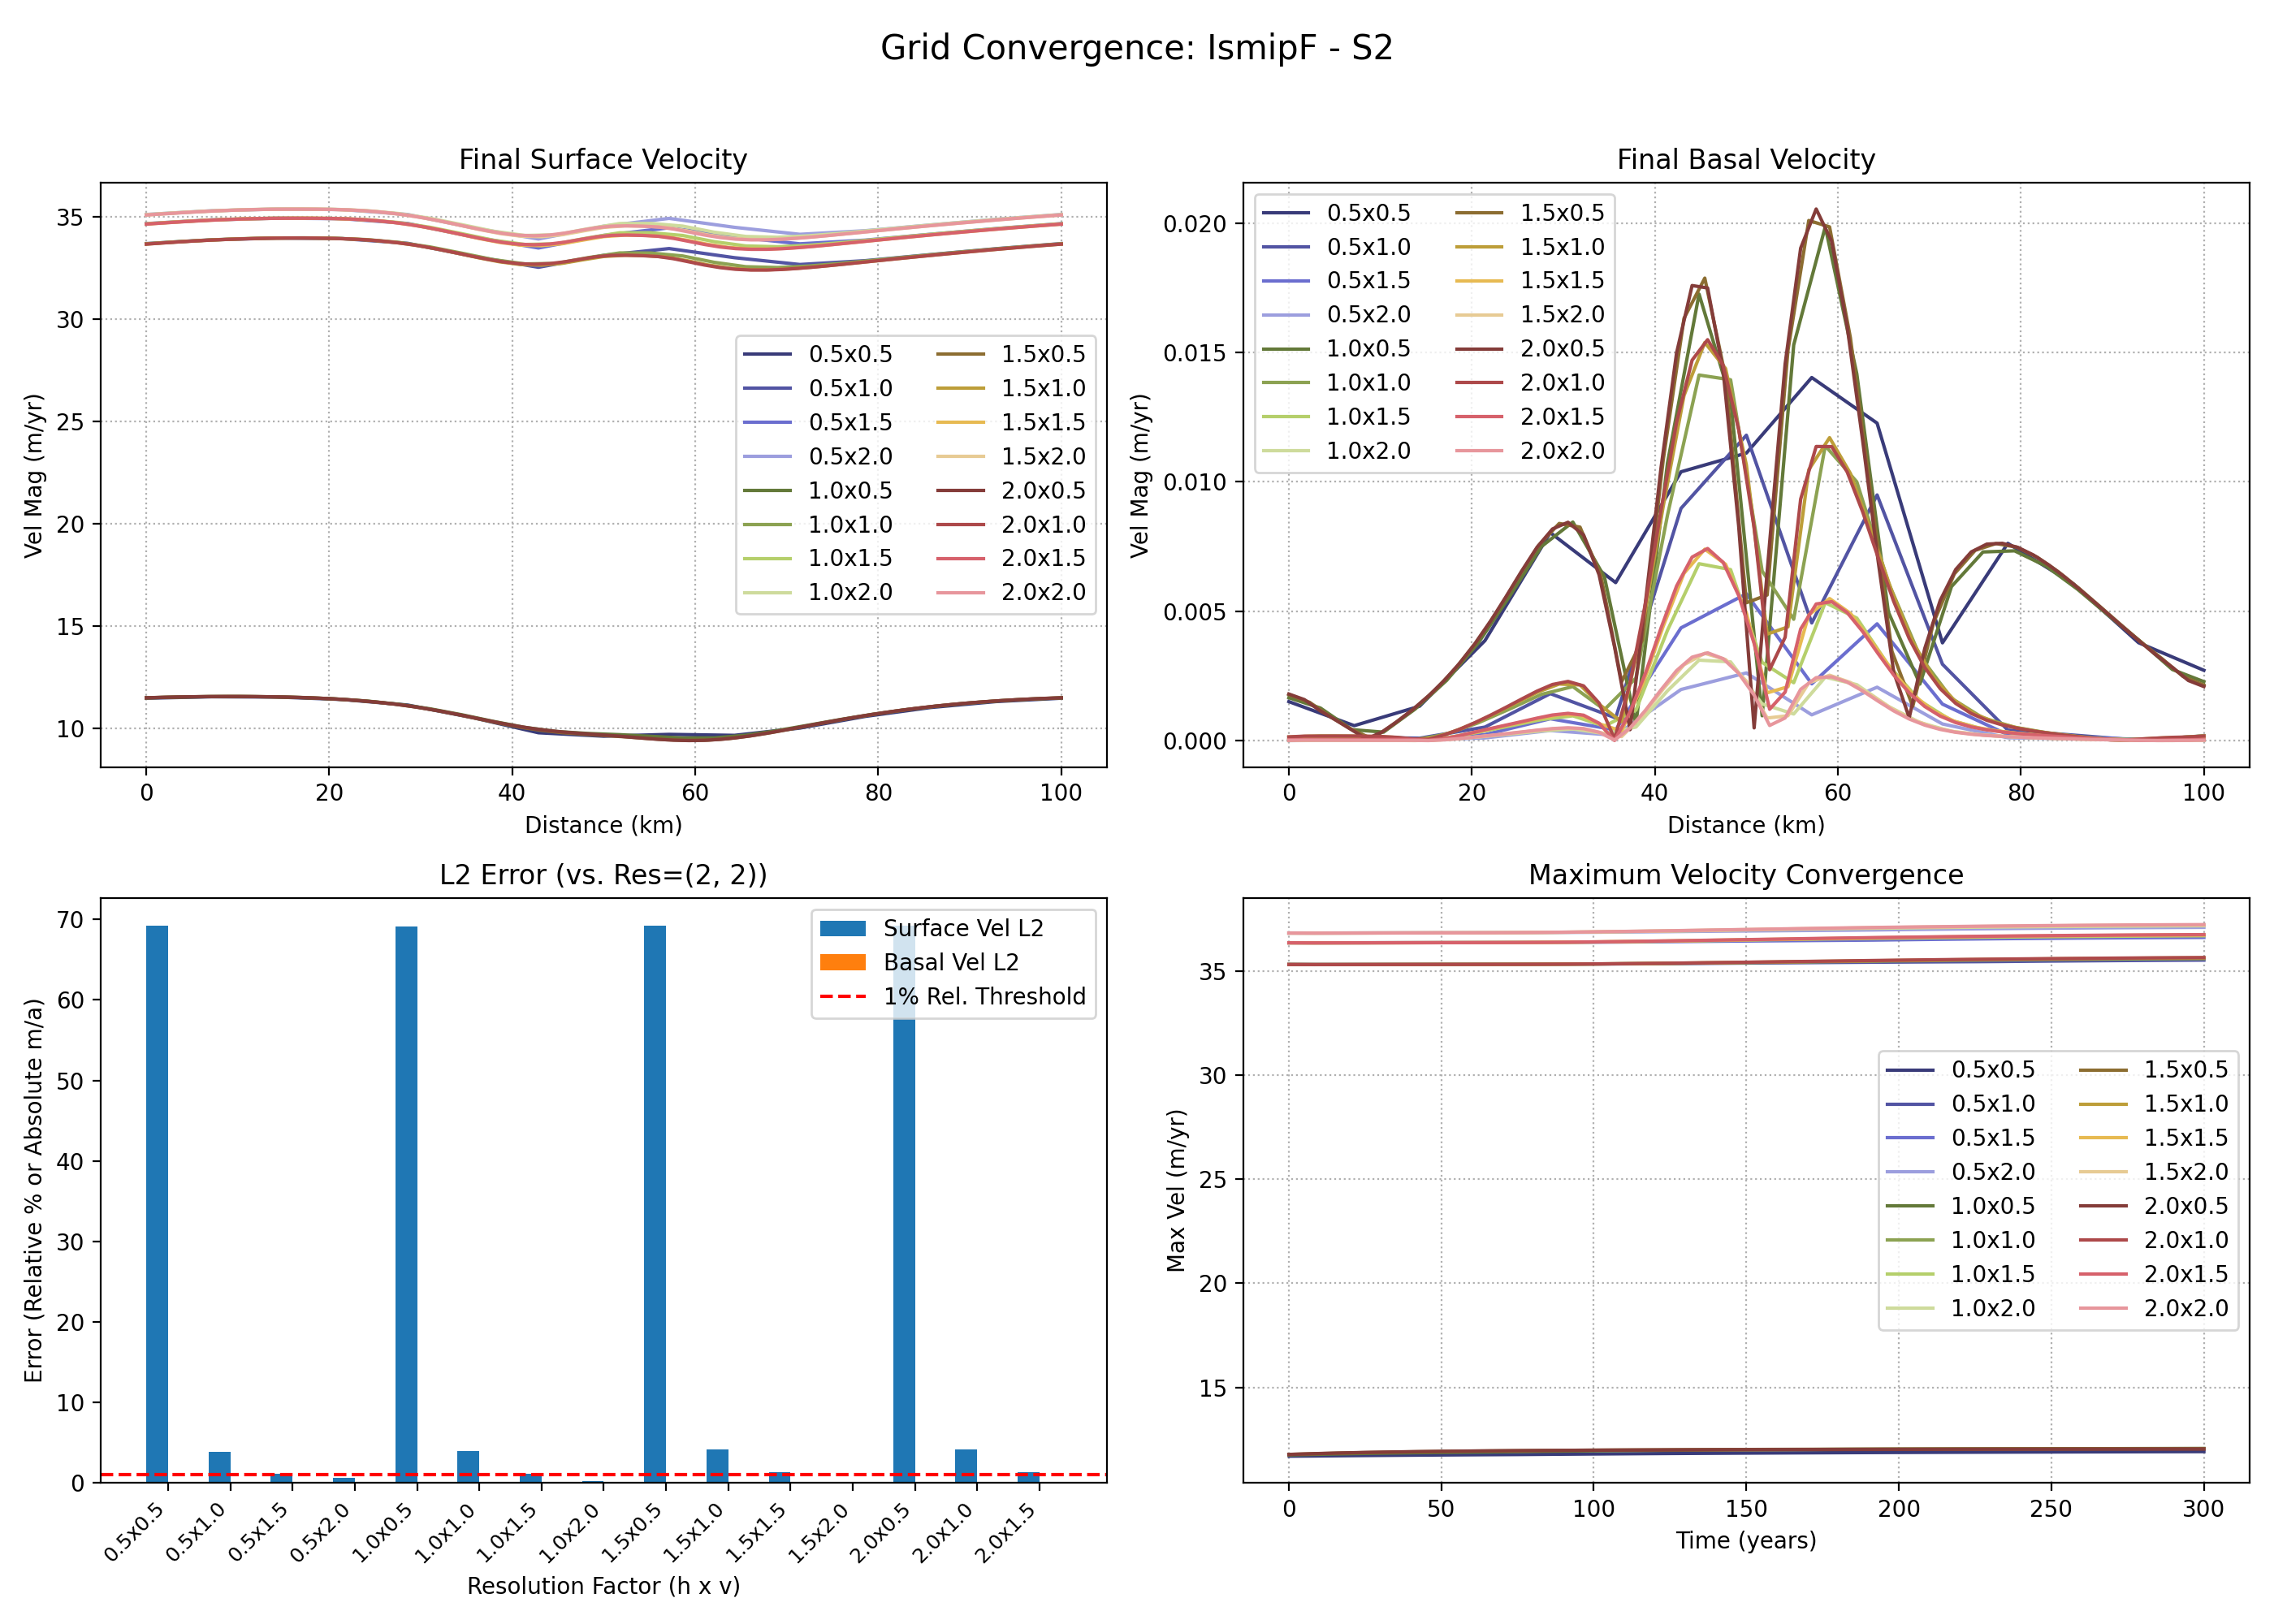
\includegraphics[scale=0.40]{figures/IsmipF_S2_convergence_summary.png}
    \caption{Grid convergence analysis for Scenario S2 (frozen bed, non-linear rheology, $n=4$). An extension of ISMIP-HOM Experiment F. The panels display the same metrics as Figure~\ref{fig:grid_conv_S1}. This scenario exhibits high sensitivity to vertical resolution refinement, with low-resolution simulations showing the highest errors and converging to a much slower flow state ($\approx~11$ m/a) compared to high-resolution runs ($\approx~37$ m/a).}
    \label{fig:grid_conv_S2}
\end{figure}
% \begin{figure}[H]
%     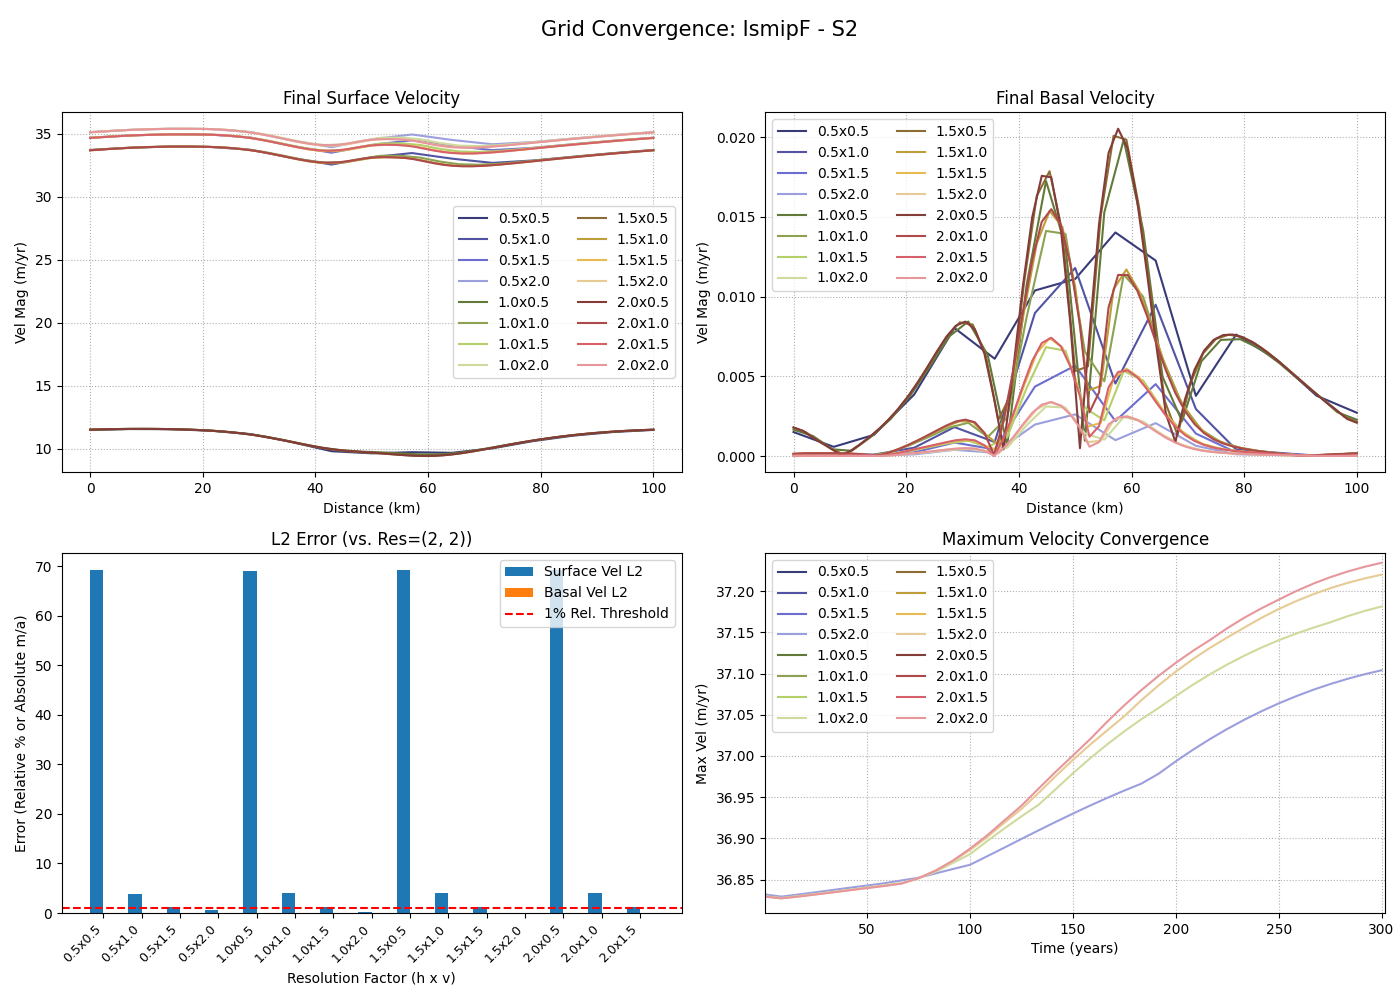
\includegraphics[scale=0.45]{figures/IsmipF_S2_convergence_summary_zoom.png}
%     \caption{}
%     \label{fig:grid_conv_S2_zoom}
% \end{figure}
\begin{figure}[H]
    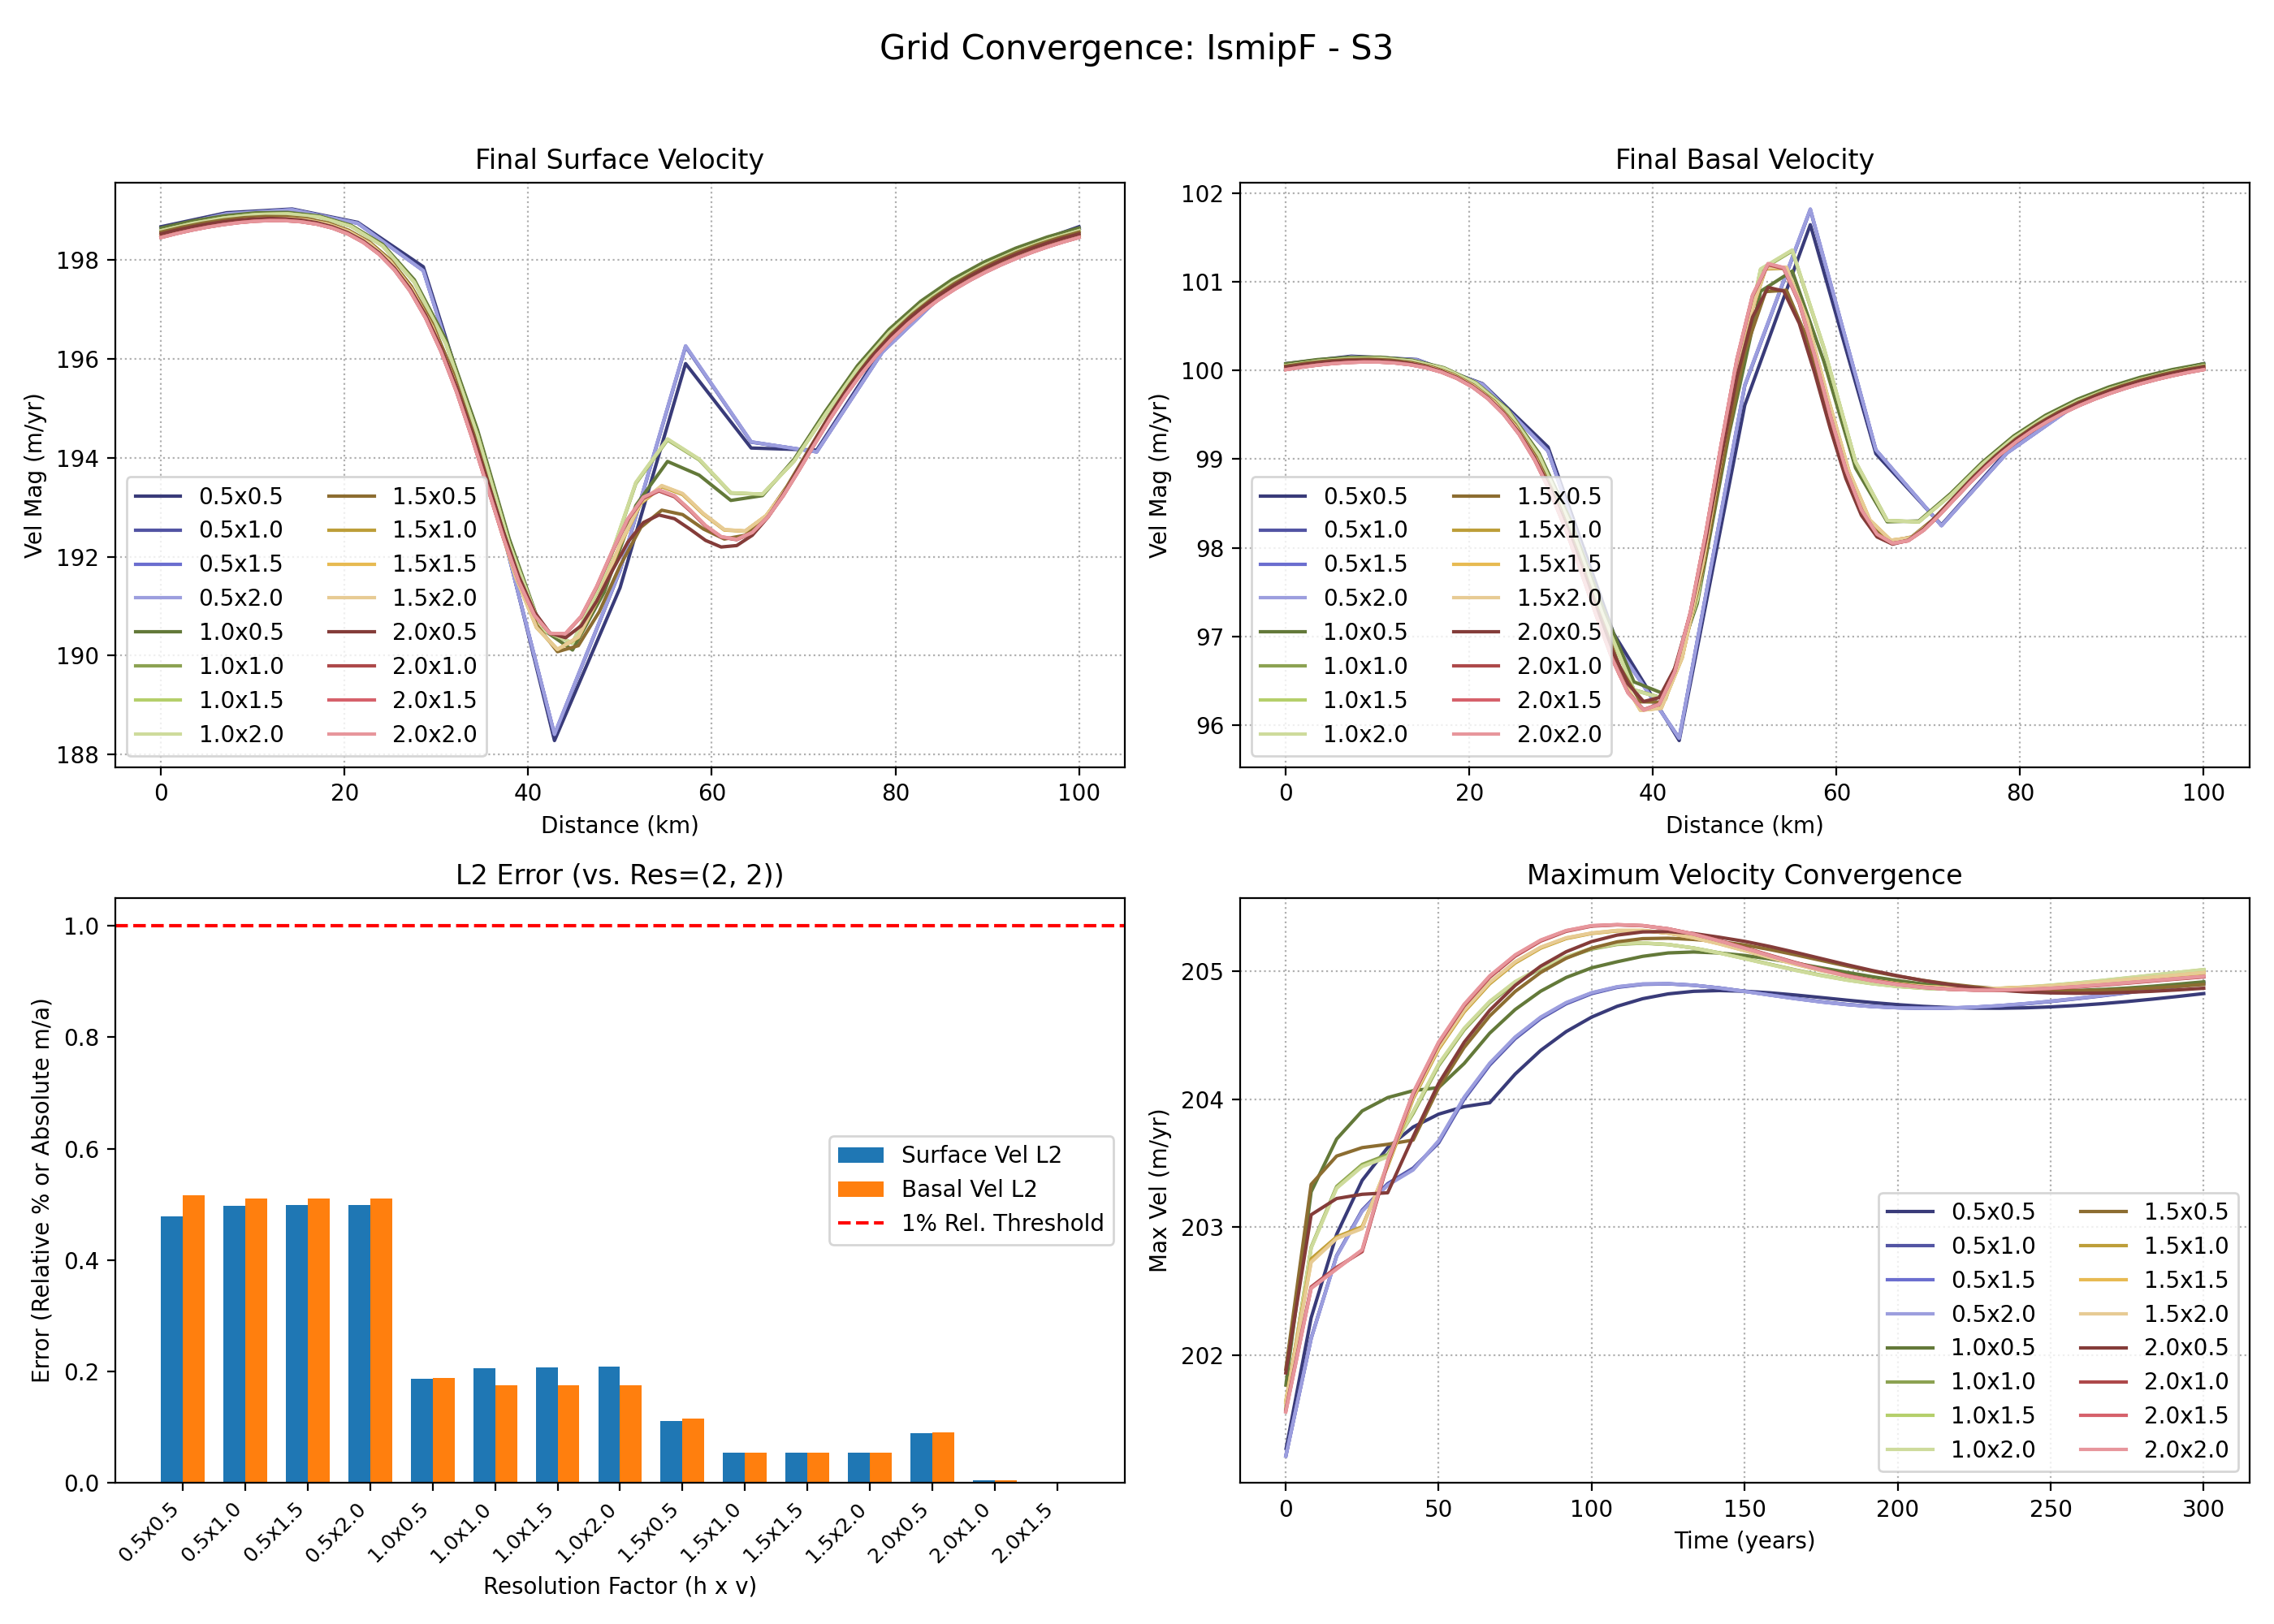
\includegraphics[scale=0.40]{figures/IsmipF_S3_convergence_summary.png}
    \caption{Grid convergence analysis for Scenario S3 (linear sliding, linear rheology, $n=1$). The four panels show: (top-left) final surface velocity profiles and (top-right) final basal velocity profiles for 16 different mesh resolutions; (bottom-left) the L2 relative error of each simulation compared to the highest-resolution mesh ($2.0\times2.0$), with a 1\% relative error threshold indicated by the dashed line; and (bottom-right) the evolution of the maximum velocity over the 300-year simulation period}
    \label{fig:grid_conv_S3}
\end{figure}
\begin{figure}[H]
    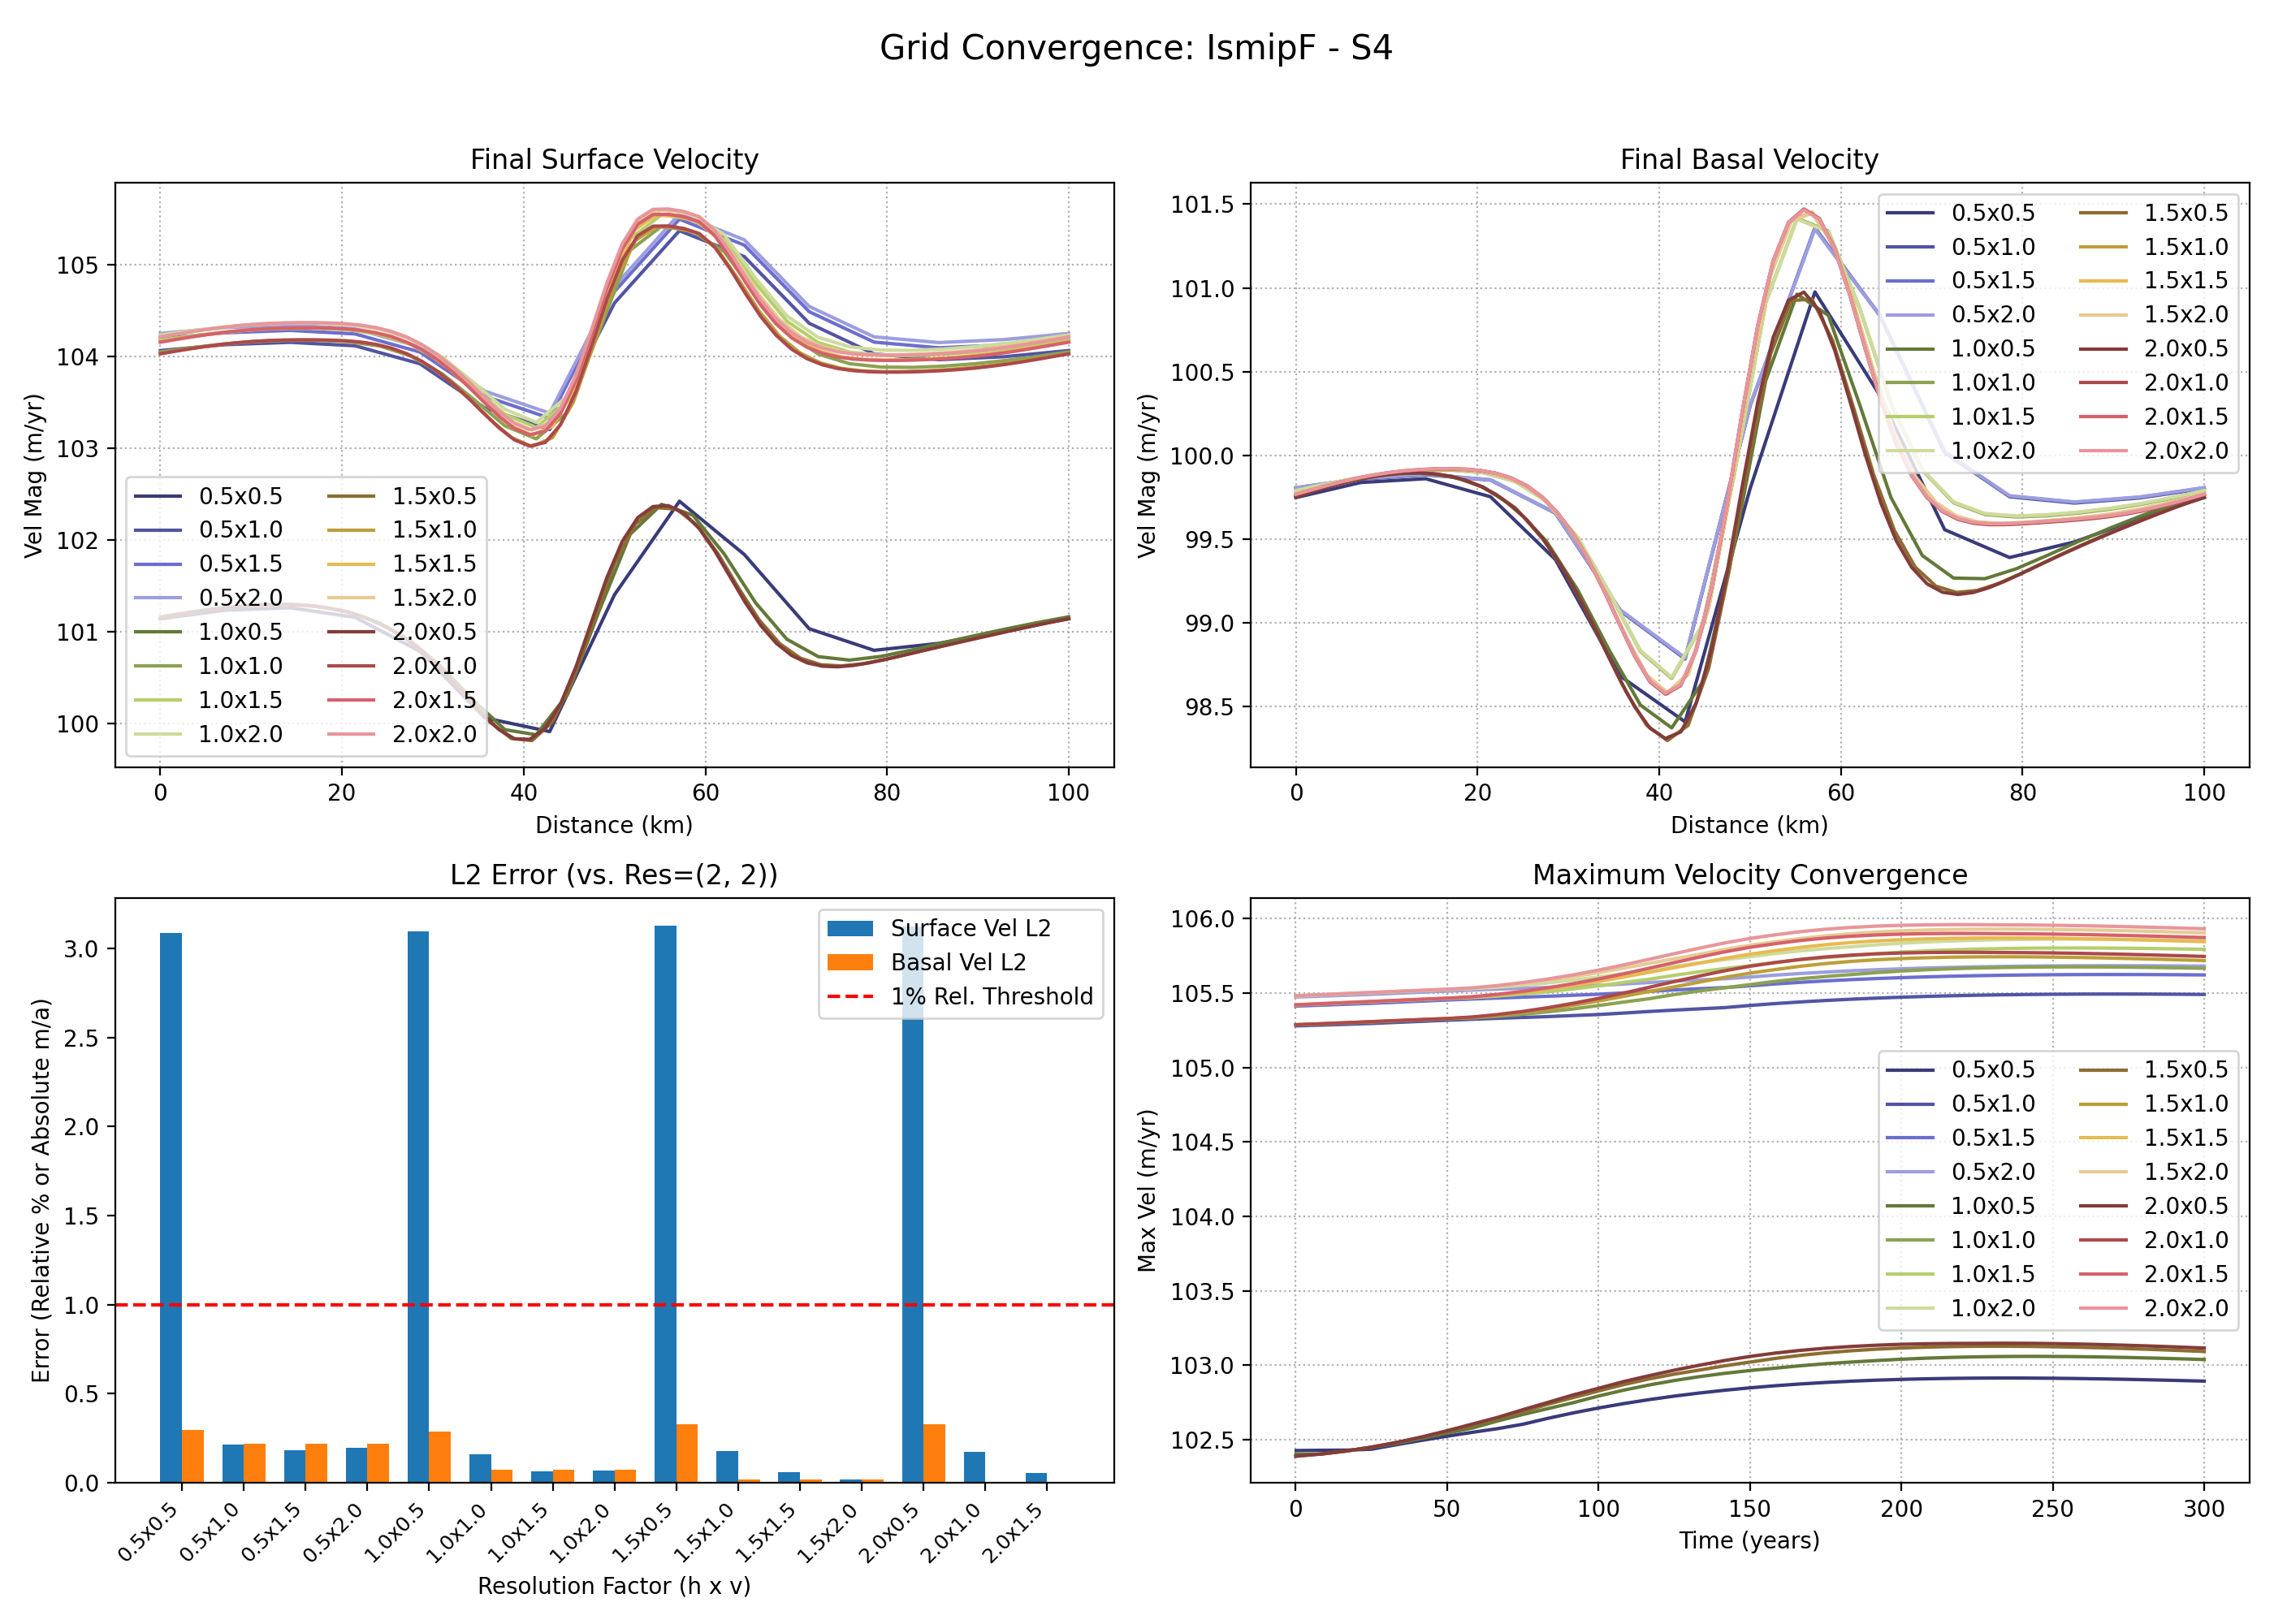
\includegraphics[scale=0.40]{figures/IsmipF_S4_convergence_summary.png}
    \caption{Grid convergence analysis for Scenario S4 (linear sliding, non-linear rheology, $n=4$). Another extension of ISMIP-HOM Experiment F, similarly to the other non-linear case (S2) in Figure~\ref{fig:grid_conv_S2}, this scenario is highly sensitive to vertical resolution. The convergence analysis shows that the 1\% relative error threshold is only achieved for simulations using the highest vertical resolution factor (2.0)}
    \label{fig:grid_conv_S4}
\end{figure}
% \begin{figure}[H]
%     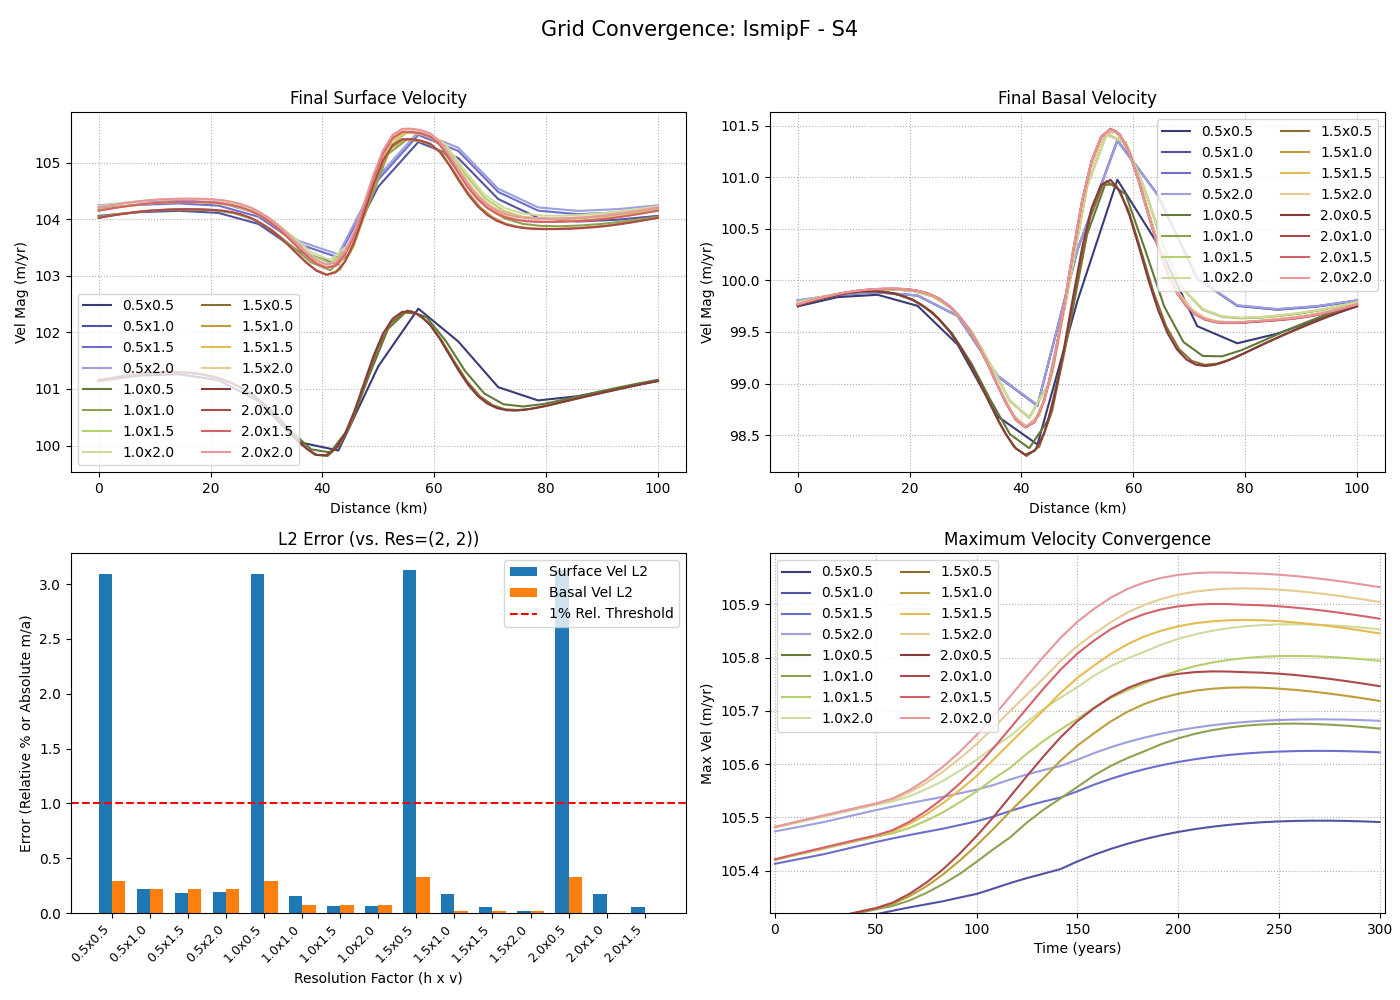
\includegraphics[scale=0.45]{figures/IsmipF_S4_convergence_summary_zoom.png}
%     \caption{}
%     \label{fig:grid_conv_S4_zoom}
% \end{figure}
My diagnostic convergence analyses show that the simulations are most sensitive to vertical resolution refinement. The effect is more dramatic with the non-linear rheology scenarios in Figures~\ref{fig:grid_conv_S2} and~\ref{fig:grid_conv_S4}. The convergence threshold of 1\% is only achieved for both S2 and S4 with the vertical resolution factor $2.0$. The vertical resolution of the mesh produces qualitatively different results as it is refined. The lowest vertical resolution simulations converge to a slow-flowing state ($\approx11 \mathrm{m/a}$). On the other hand the high- vertical resolution simulations converge to larger velocities ($\approx37\mathrm{m/a}$).  In addition to this, the Frozen bed scenario S2 basal velocities show the highest errors for low resolution simulations. 
% \subsubsection{Mesh and Transient Fields}
% % # ALSO INCLUDE EXTRACT RESULTS???
% % THESE ARE ONLY FOR THE CHOSEN FINAL RESOLUTION
% % INITIAL MESH
% % def visual_mesh_check(md):
% % \begin{figure}[H]
% %     \includegraphics[scale=0.45]{figures/}
% %     \caption{}
% %     \label{fig:}
% % \end{figure}
% % FINAL MESH?
% % def visual_mesh_check(md):
% % \begin{figure}[H]
% %     \includegraphics[scale=0.45]{figures/}
% %     \caption{}
% %     \label{fig:}
% % \end{figure}
% % ~~~~~~~~~~~~~~~~~~~~~~~~~~~~~~~~~~~~~~~~~~~~~~~~~~~~~~~~~~~~~~~~~~~~~
% % def plot_transient_fields(md):                                                            
% % \begin{figure}[H]
% %     \includegraphics[scale=0.45]{figures/}
% %     \caption{}
% %     \label{fig:Velocity_magnitude}
% % \end{figure}
% % \begin{figure}[H]
% %     \includegraphics[scale=0.45]{figures/}
% %     \caption{}
% %     \label{fig:Pressure_magnitude}}
% % \end{figure}
% % \begin{figure}[H]
% %     \includegraphics[scale=0.45]{figures/}
% %     \caption{}
% %     \label{fig:base_surface_elevation_magnitude}
% % \end{figure}
% % ~~~~~~~~~~~~~~~~~~~~~~~~~~~~~~~~~~~~~~~~~~~~~~~~~~~~~~~~~~~~~~~~~~~~~
% % def plot_max_velocity_from_netcdf(filename):
% % \begin{figure}[H]
% %     \includegraphics[scale=0.45]{figures/}
% %     \caption{}
% %     \label{fig:}
% % \end{figure}

% % def diagnose_acceleration_onset(md, L)://////////????????
% % \begin{figure}[H]
% %     \includegraphics[scale=0.45]{figures/}
% %     \caption{}
% %     \label{fig:}
% % \end{figure}
% % ======================================================
\subsubsection{Phase Analysis}
I developed single and batch-processing scripts (e.g. \texttt{phase\_analysis.py}) to directly quantify the the bed-to-surface phase signal transfer. This analysis provides a metric to verify that my model's physics are consistent with the criteria in~\cite{Budd_1970}. Who predicted a phase shift of approximately $\pi / 2$. 
My phase analysis tracks the evolution of the surface with respect to the base and uses cross-correlation to calculate the spatial lag and phase shift between the de-trended signals for each time step in a given simulation.
The scripts generate time-series plots of phase shift evolution and summary text files with numerical results. For each batch or single simulation analysed.
The code deduces key simulation parameters like the parameter profile, experimental scenario, and mesh resolution scaling factors from the name of the NetCDF script being analysed, then it configures and reconstructs the original model setup and mesh exactly as it was during the simulation run. For visualisation purposes, for each time step recorded in the NetCDF file the script extracts a 1D profile of the ice base and surface elevations along a user-defined line (e.g., along the x-axis at the domain's centre). The core of the analysis is to separate the "signal" (the topographic bump) from the "background" (the unperturbed, sloping ice sheet). It does this by calculating the theoretical baseline for the bed and surface and subtracting it from the actual elevations. To find the shift between the bedrock signal and the surface signal, the script uses cross-correlation (\texttt{scipy.signal.correlate}), the peak of this function corresponds to the spatial lag where the two signals are most similar.
The spatial lag is converted into a phase shift in degrees using the bedrock's characteristic wavelength from the parameter file. These analysis steps are repeated for every time step in the simulation. The script stores the phase shift and lag distance for each point in time, allowing it to generate plots that show how the phase relationship evolves.
%%%% S1
\begin{figure}[H]
    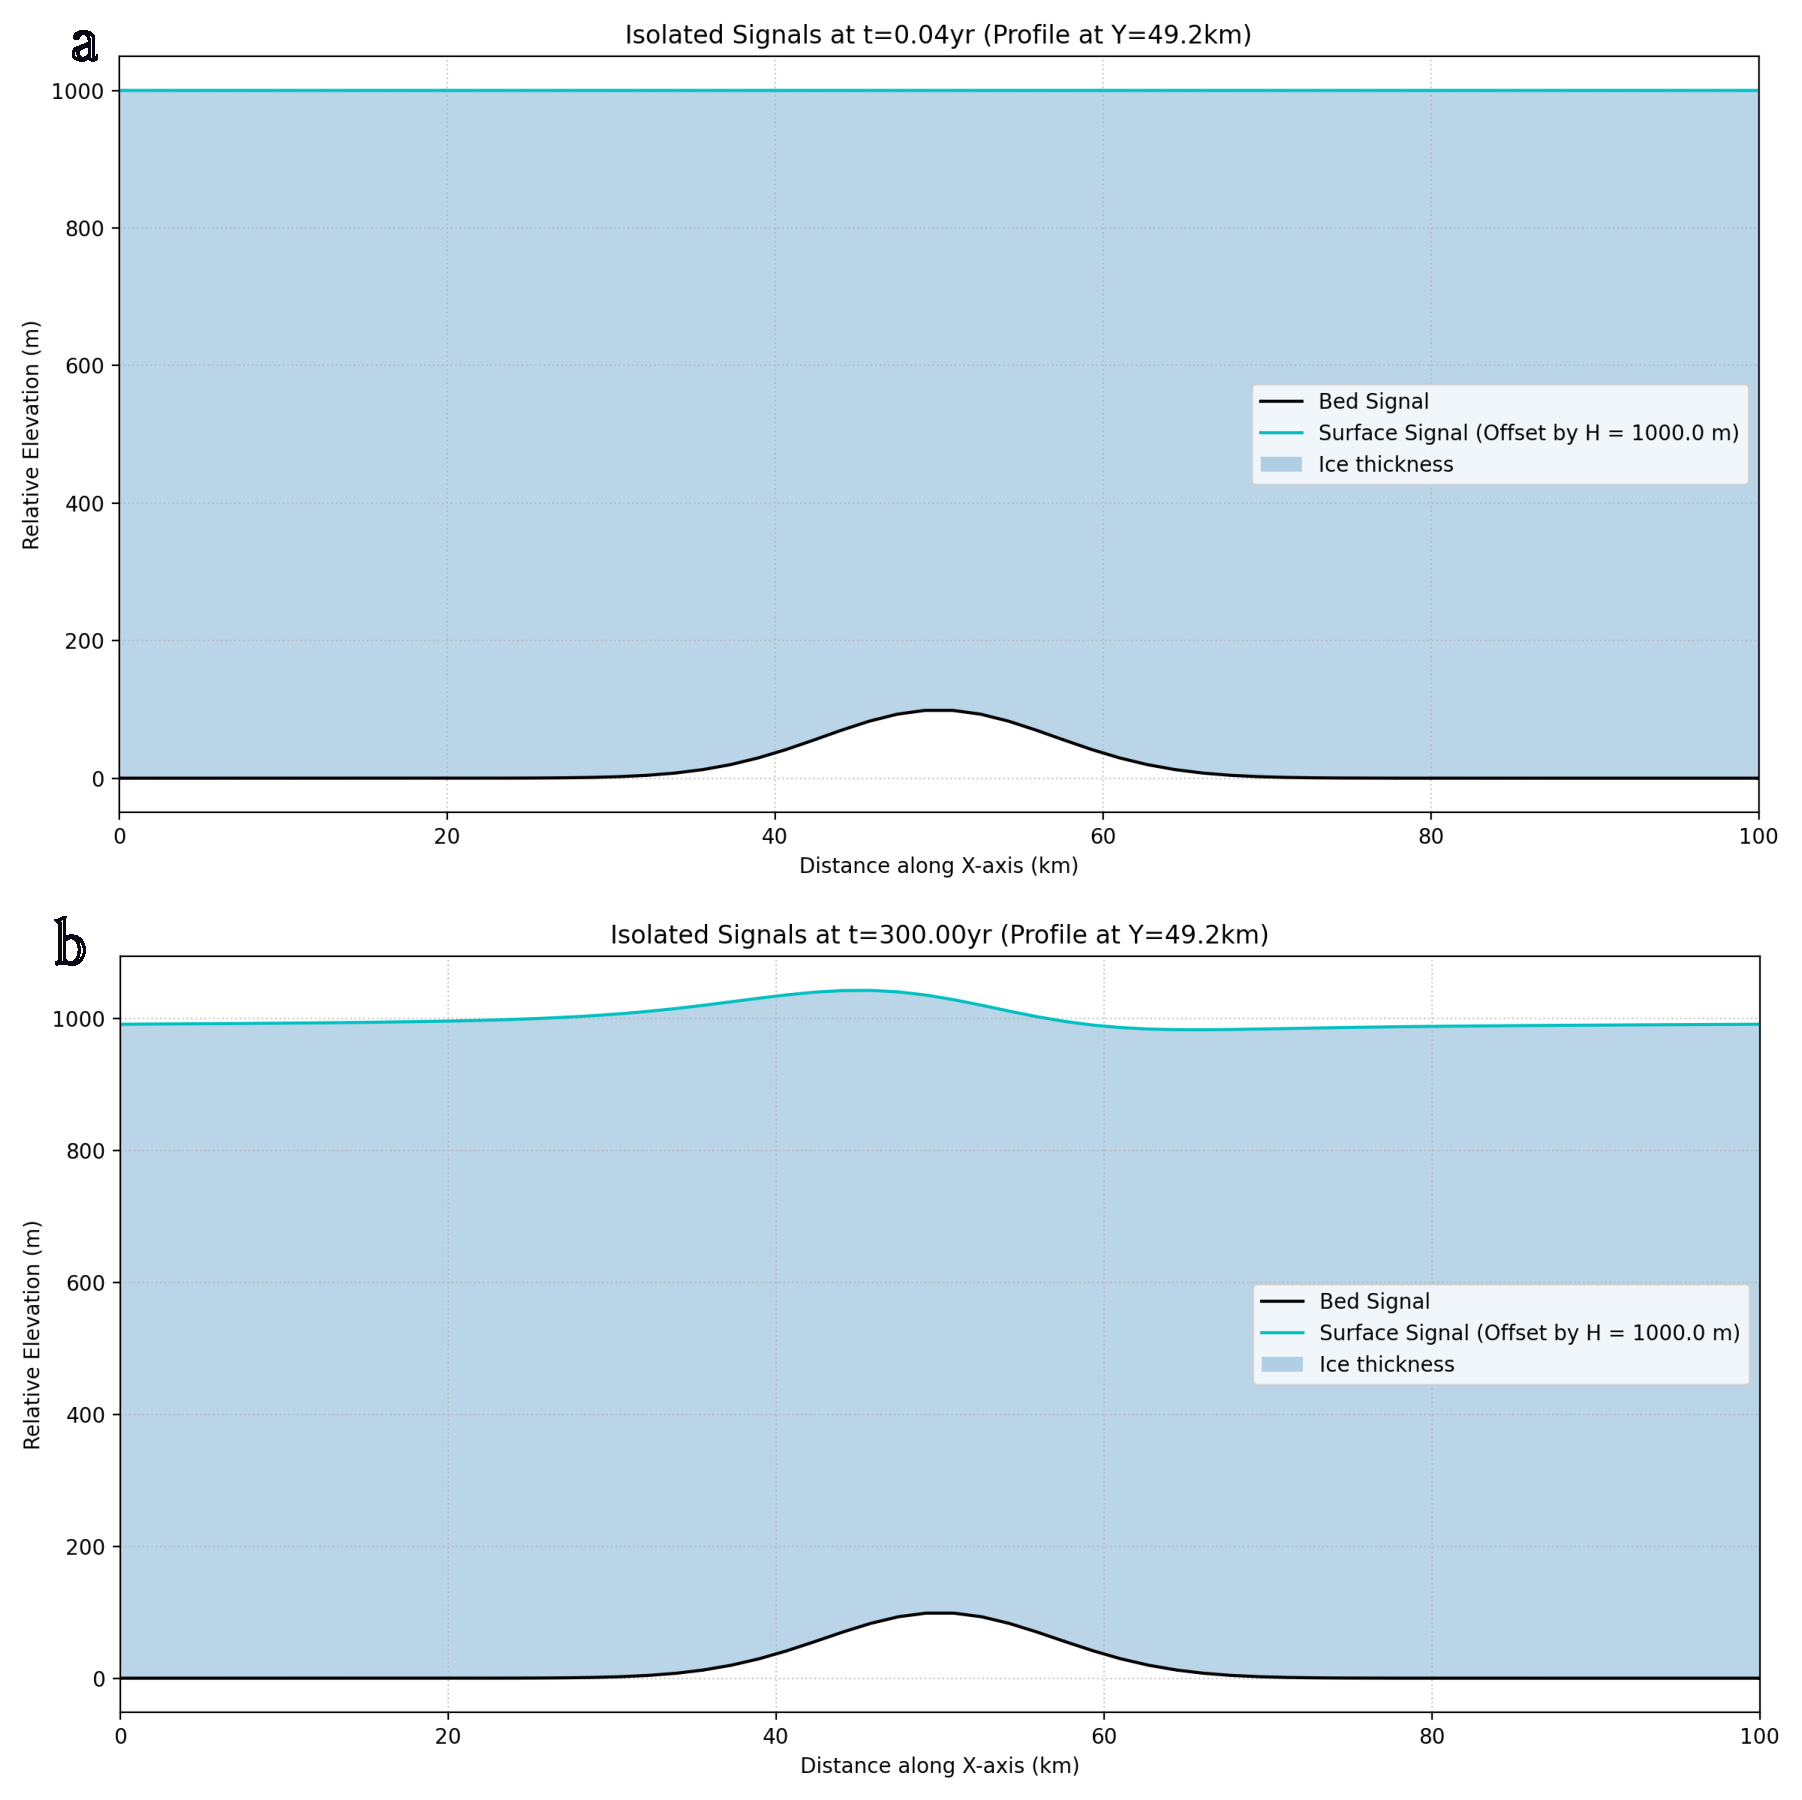
\includegraphics[scale=0.30]{figures/S1_F_signals.pdf}
    \caption{The isolated bedrock and ice surface signals (along the y- centreline) for the initial (a) and final (b) time steps in the 300 year long simulation. The bedrock is identical to that of ISMIP HOM experiment F (S1: Frozen bed and linear rheology). As time progresses and the ice surface responds to the underlying bed topography, the surface develops a bump that's spatially shifted relative to the bed bump (upstream due to ice flow dynamics).}
    \label{fig:phase_analysis_Signals}
\end{figure}
% \begin{figure}[H]
%     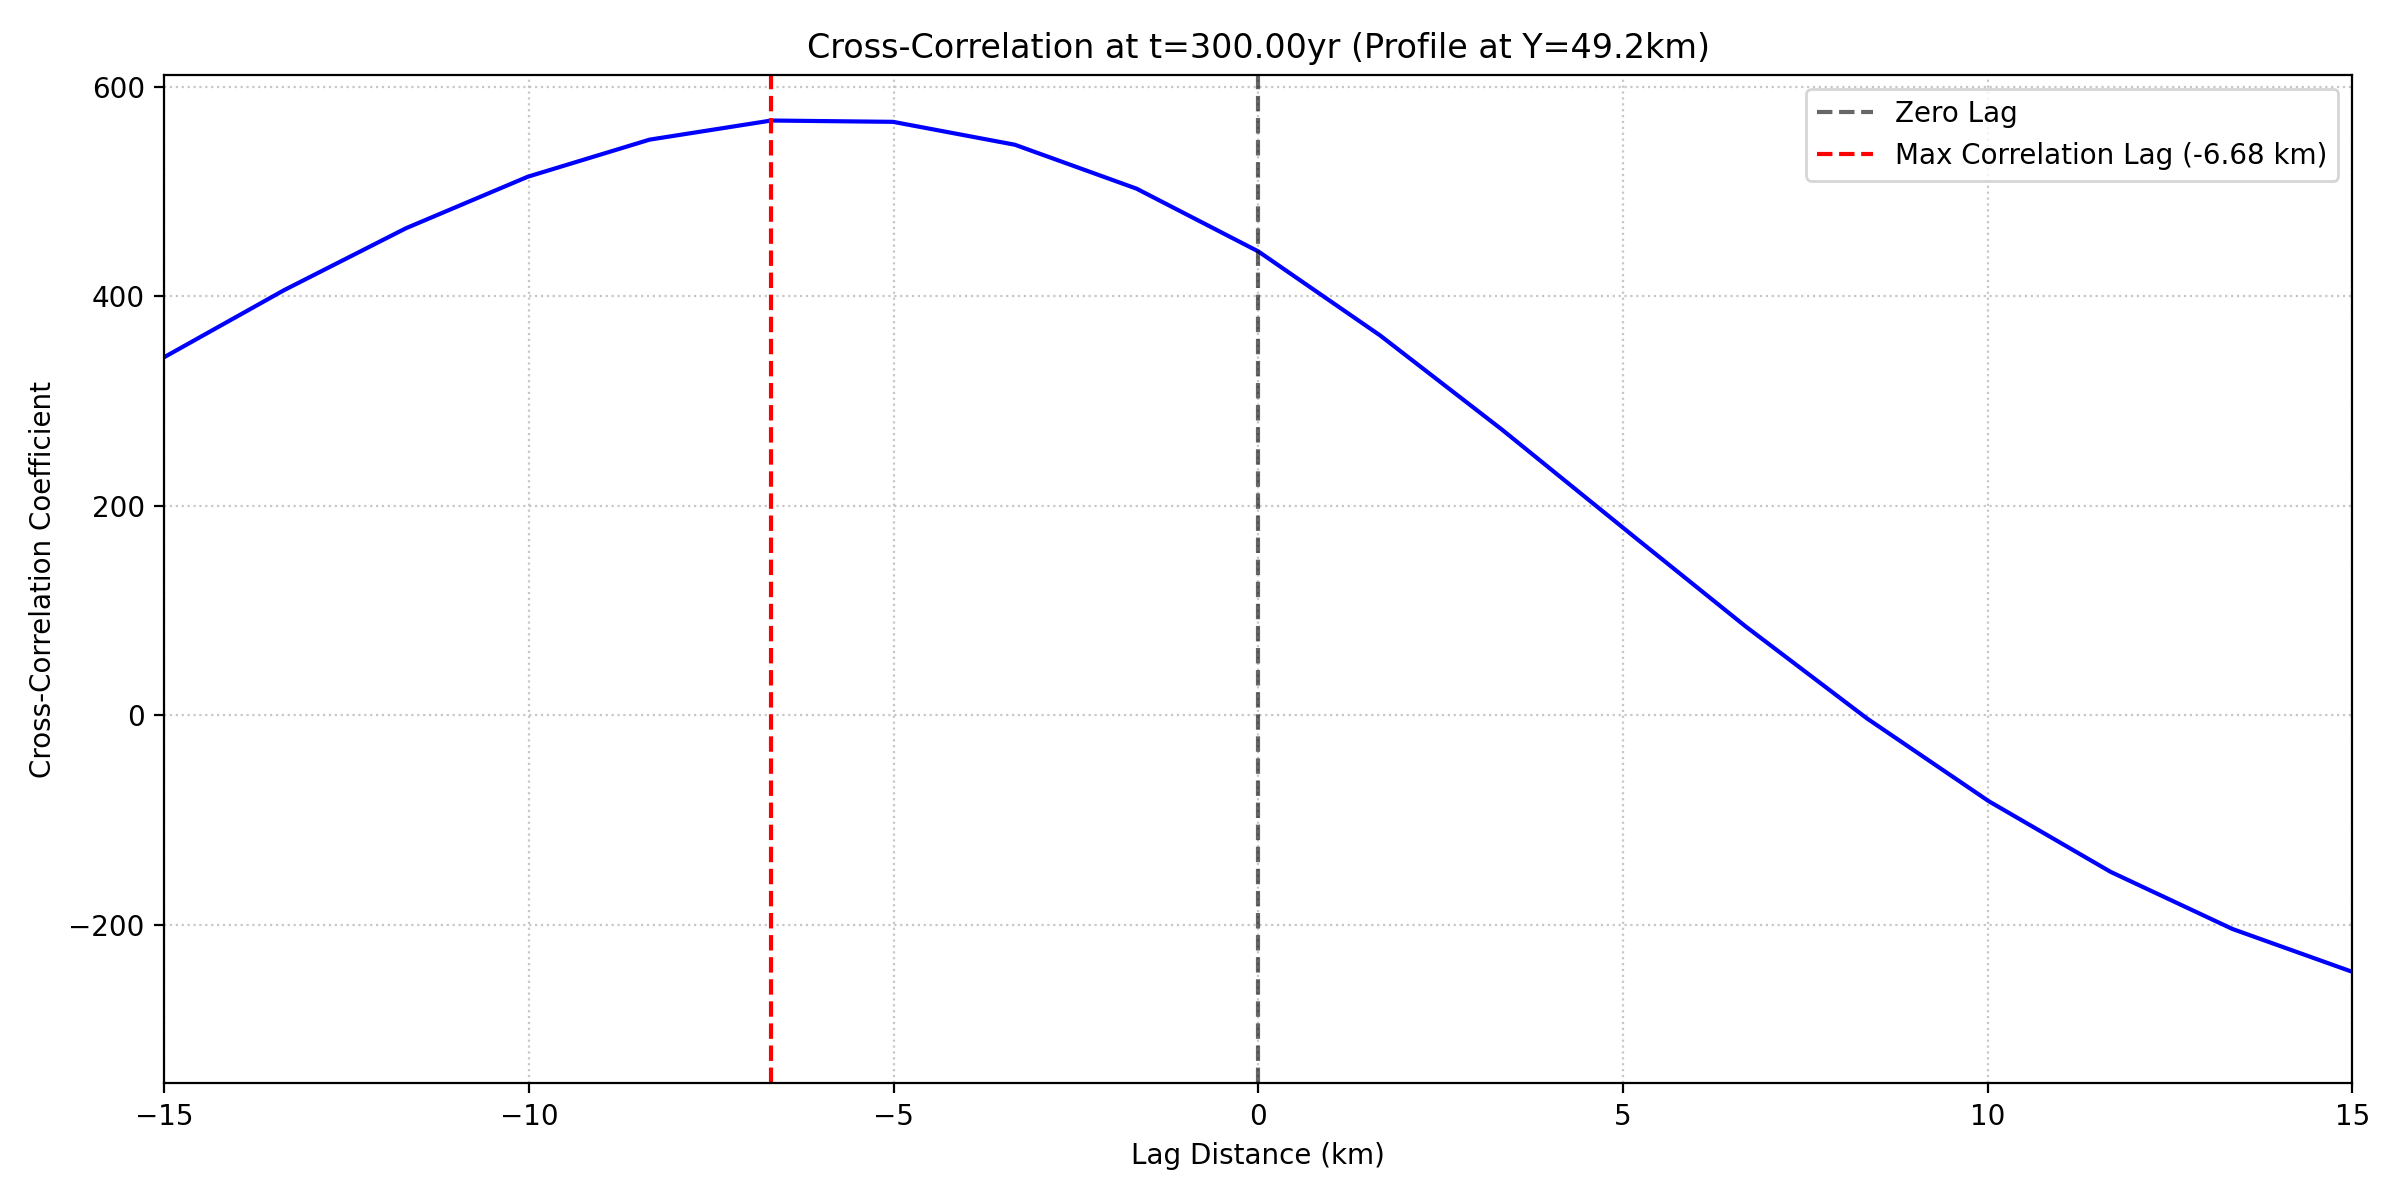
\includegraphics[scale=0.30]{figures/S1_F_correlation_t_0036.png}
%     \caption{The cross-correlation of surface and bed elevation signals shift relative to the most prominent bed feature, using sigma (the Gaussian width) as the characteristic length scale of the lag.}
%     \label{fig:phase_analysis_Cross_Correlation}
% \end{figure}
\begin{figure}[H]
    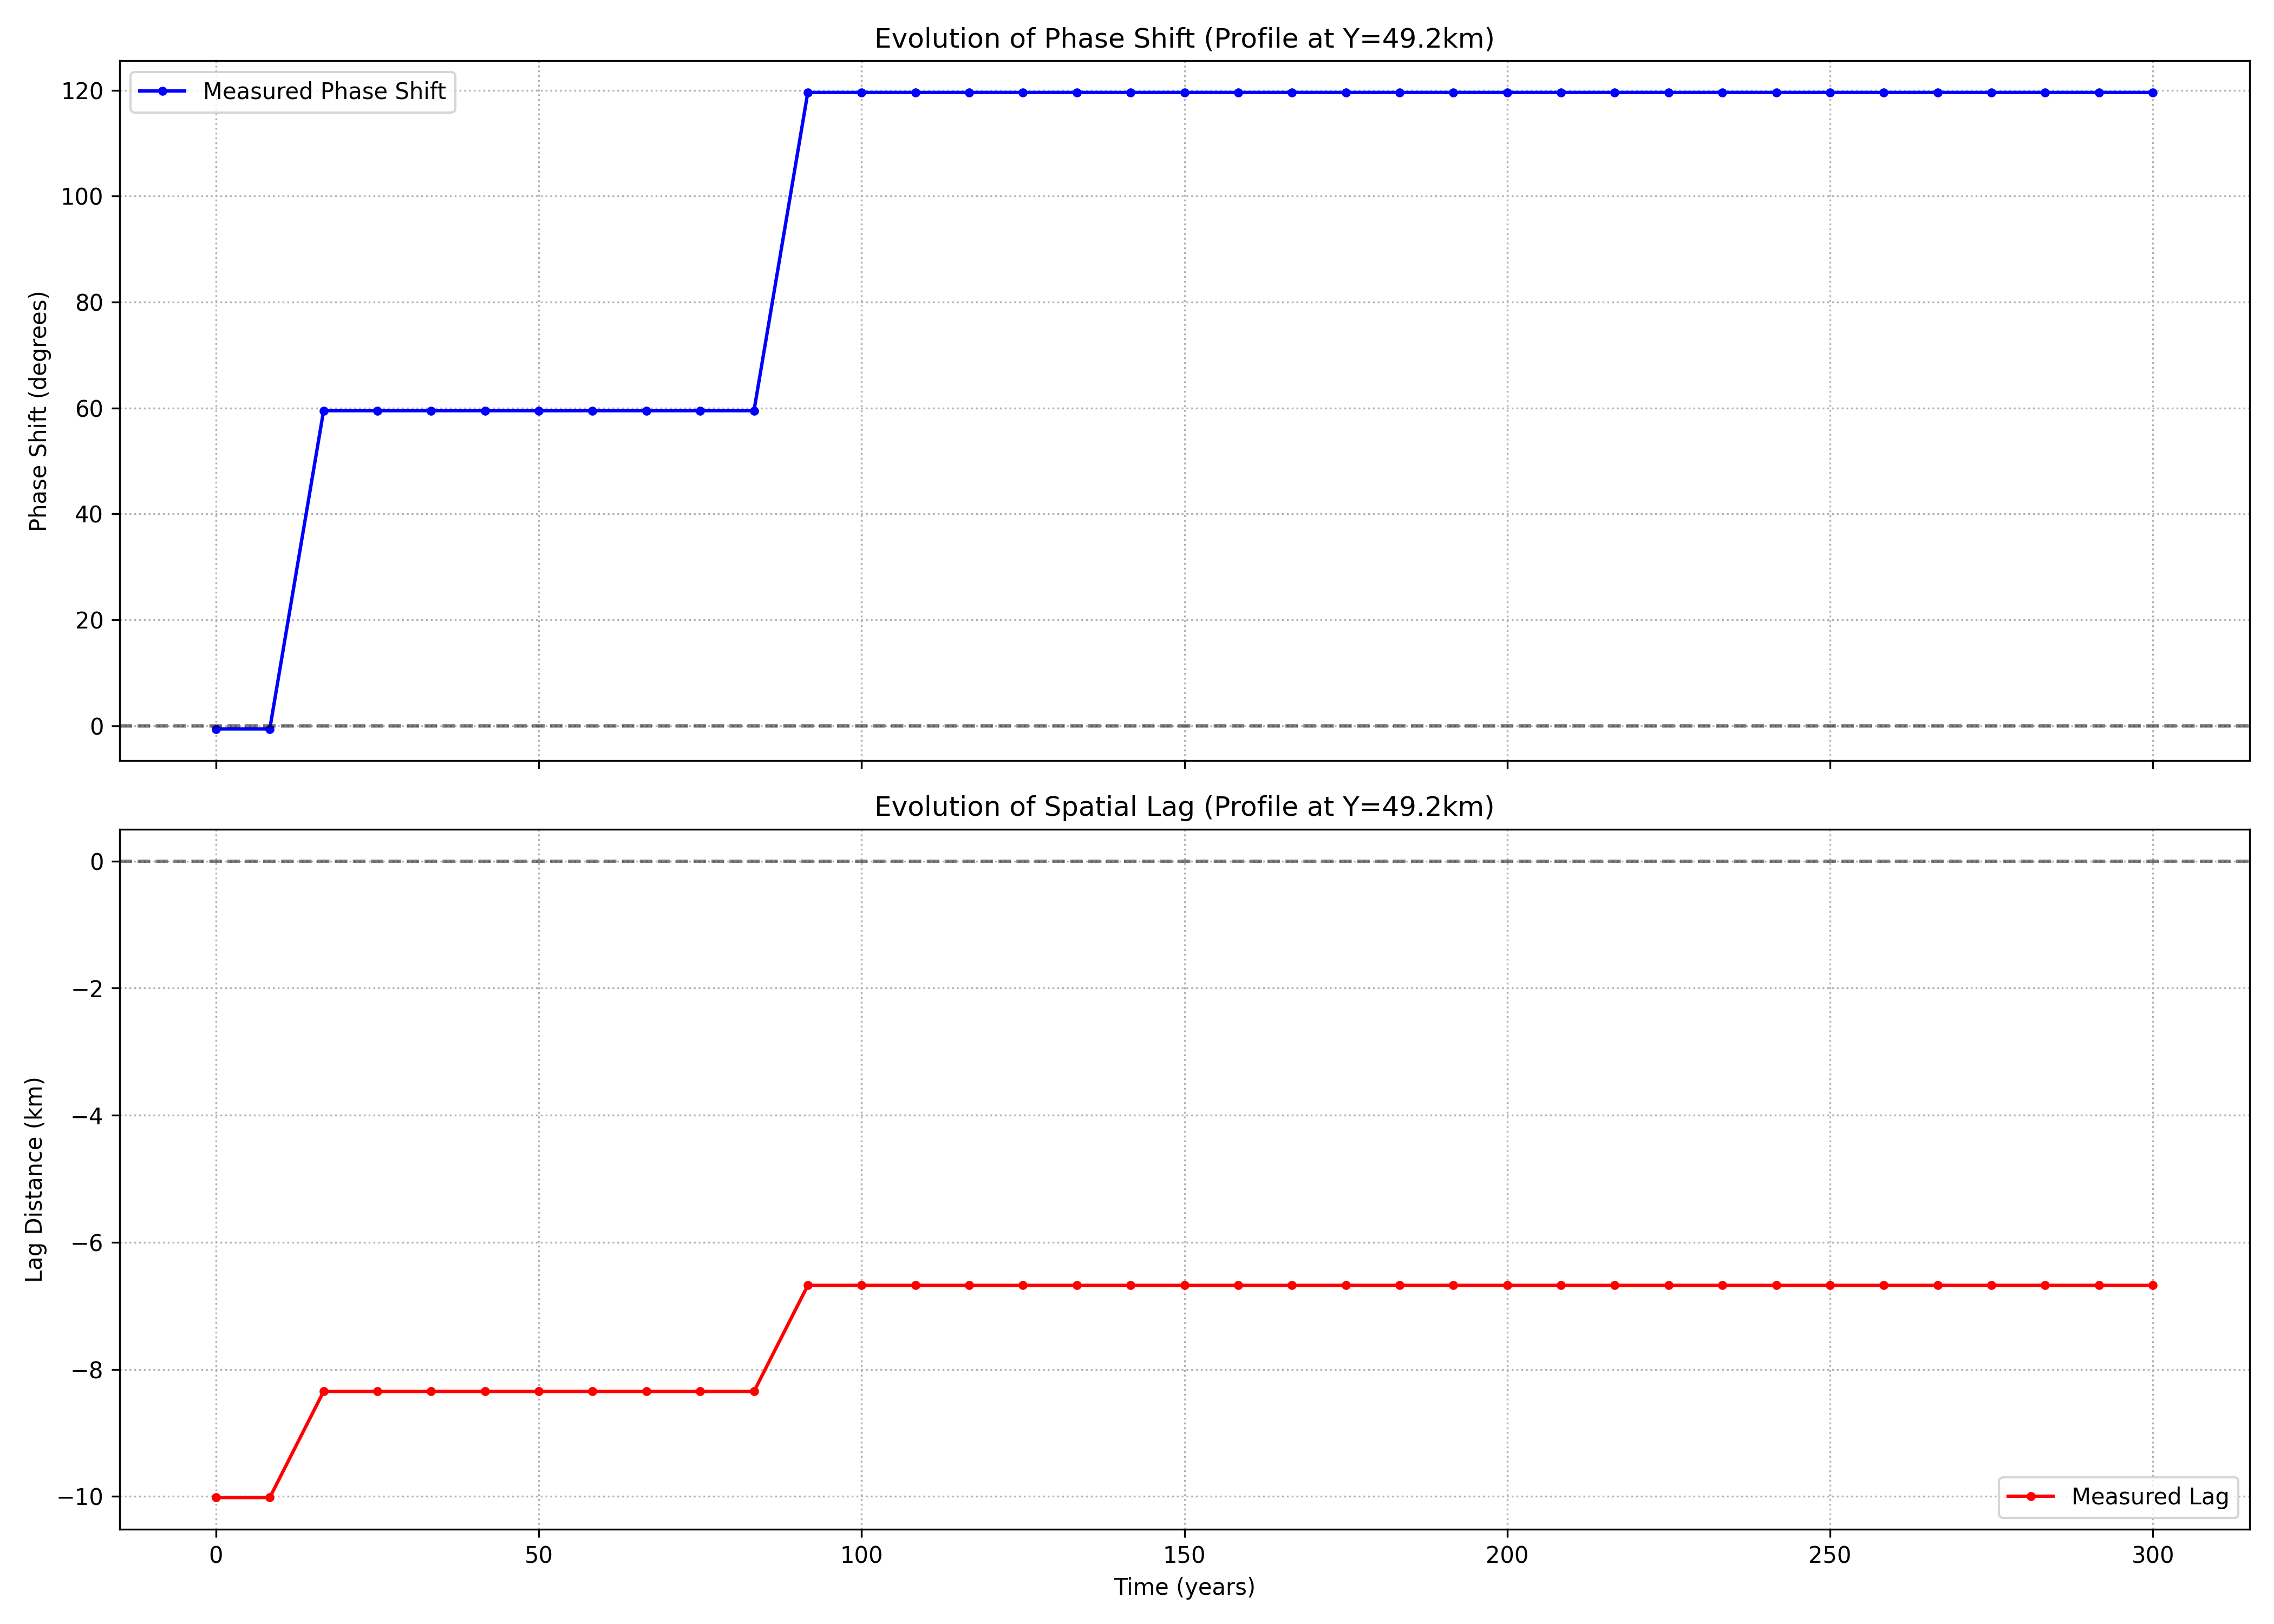
\includegraphics[scale=0.30]{figures/S1_F_phase_evolution_summary.png}
    \caption{The evolution of the phase shift and spatial lag over the entire simulation.}
    \label{fig:phase_analysis_Evolution_Plots}
\end{figure}
% %%% S2
% \begin{figure}[H]
%     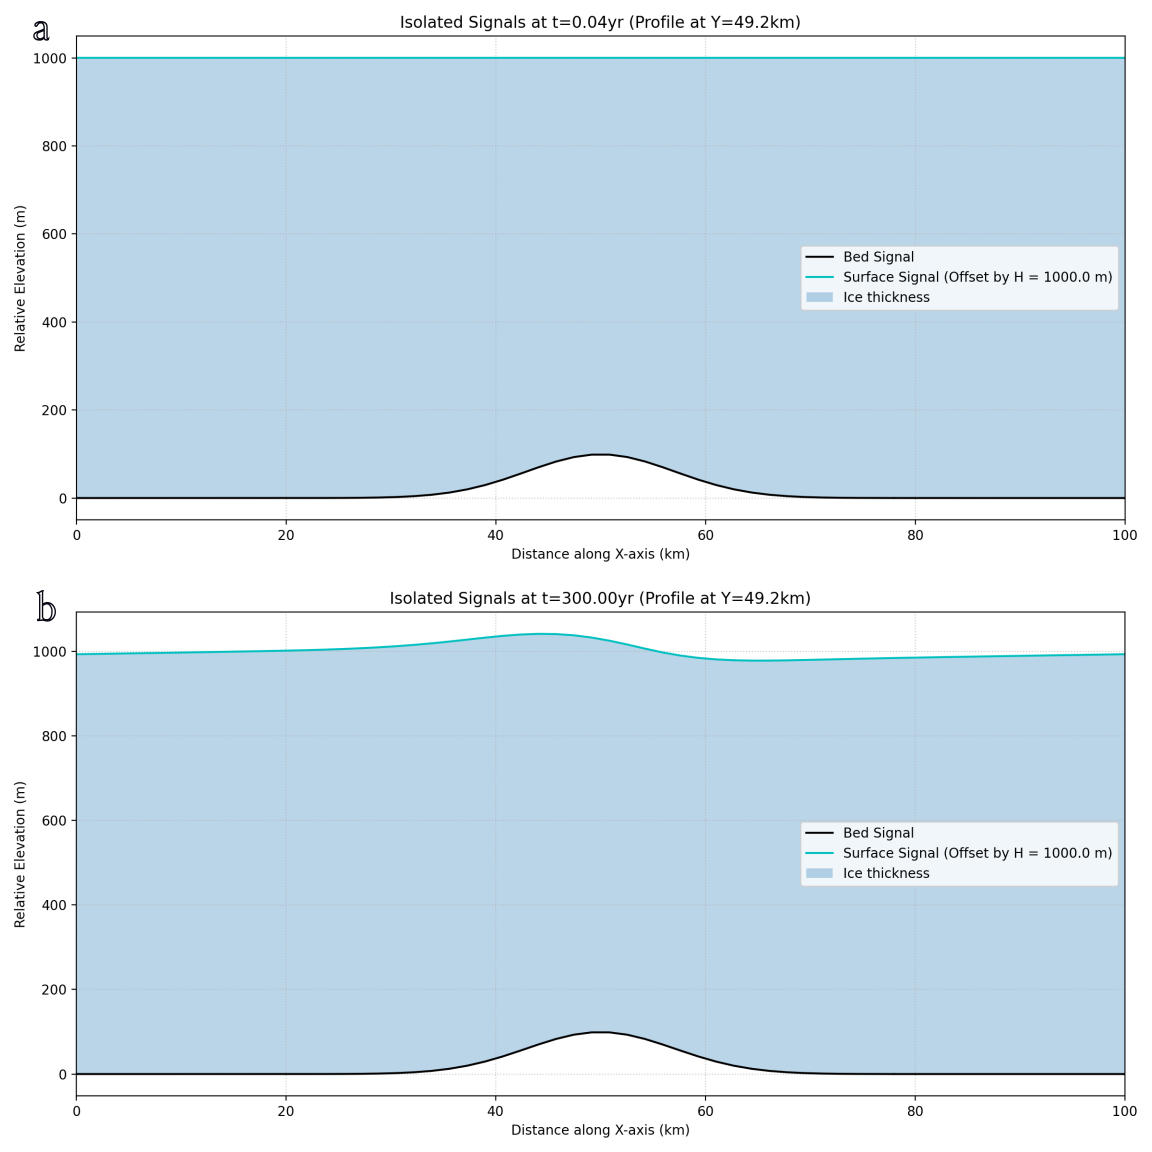
\includegraphics[scale=0.45]{figures/S2_F_signals.pdf}
%     \caption{The isolated bedrock and ice surface signals}
%     \label{fig:phase_analysis_Signals}
% \end{figure}
% \begin{figure}[H]
%     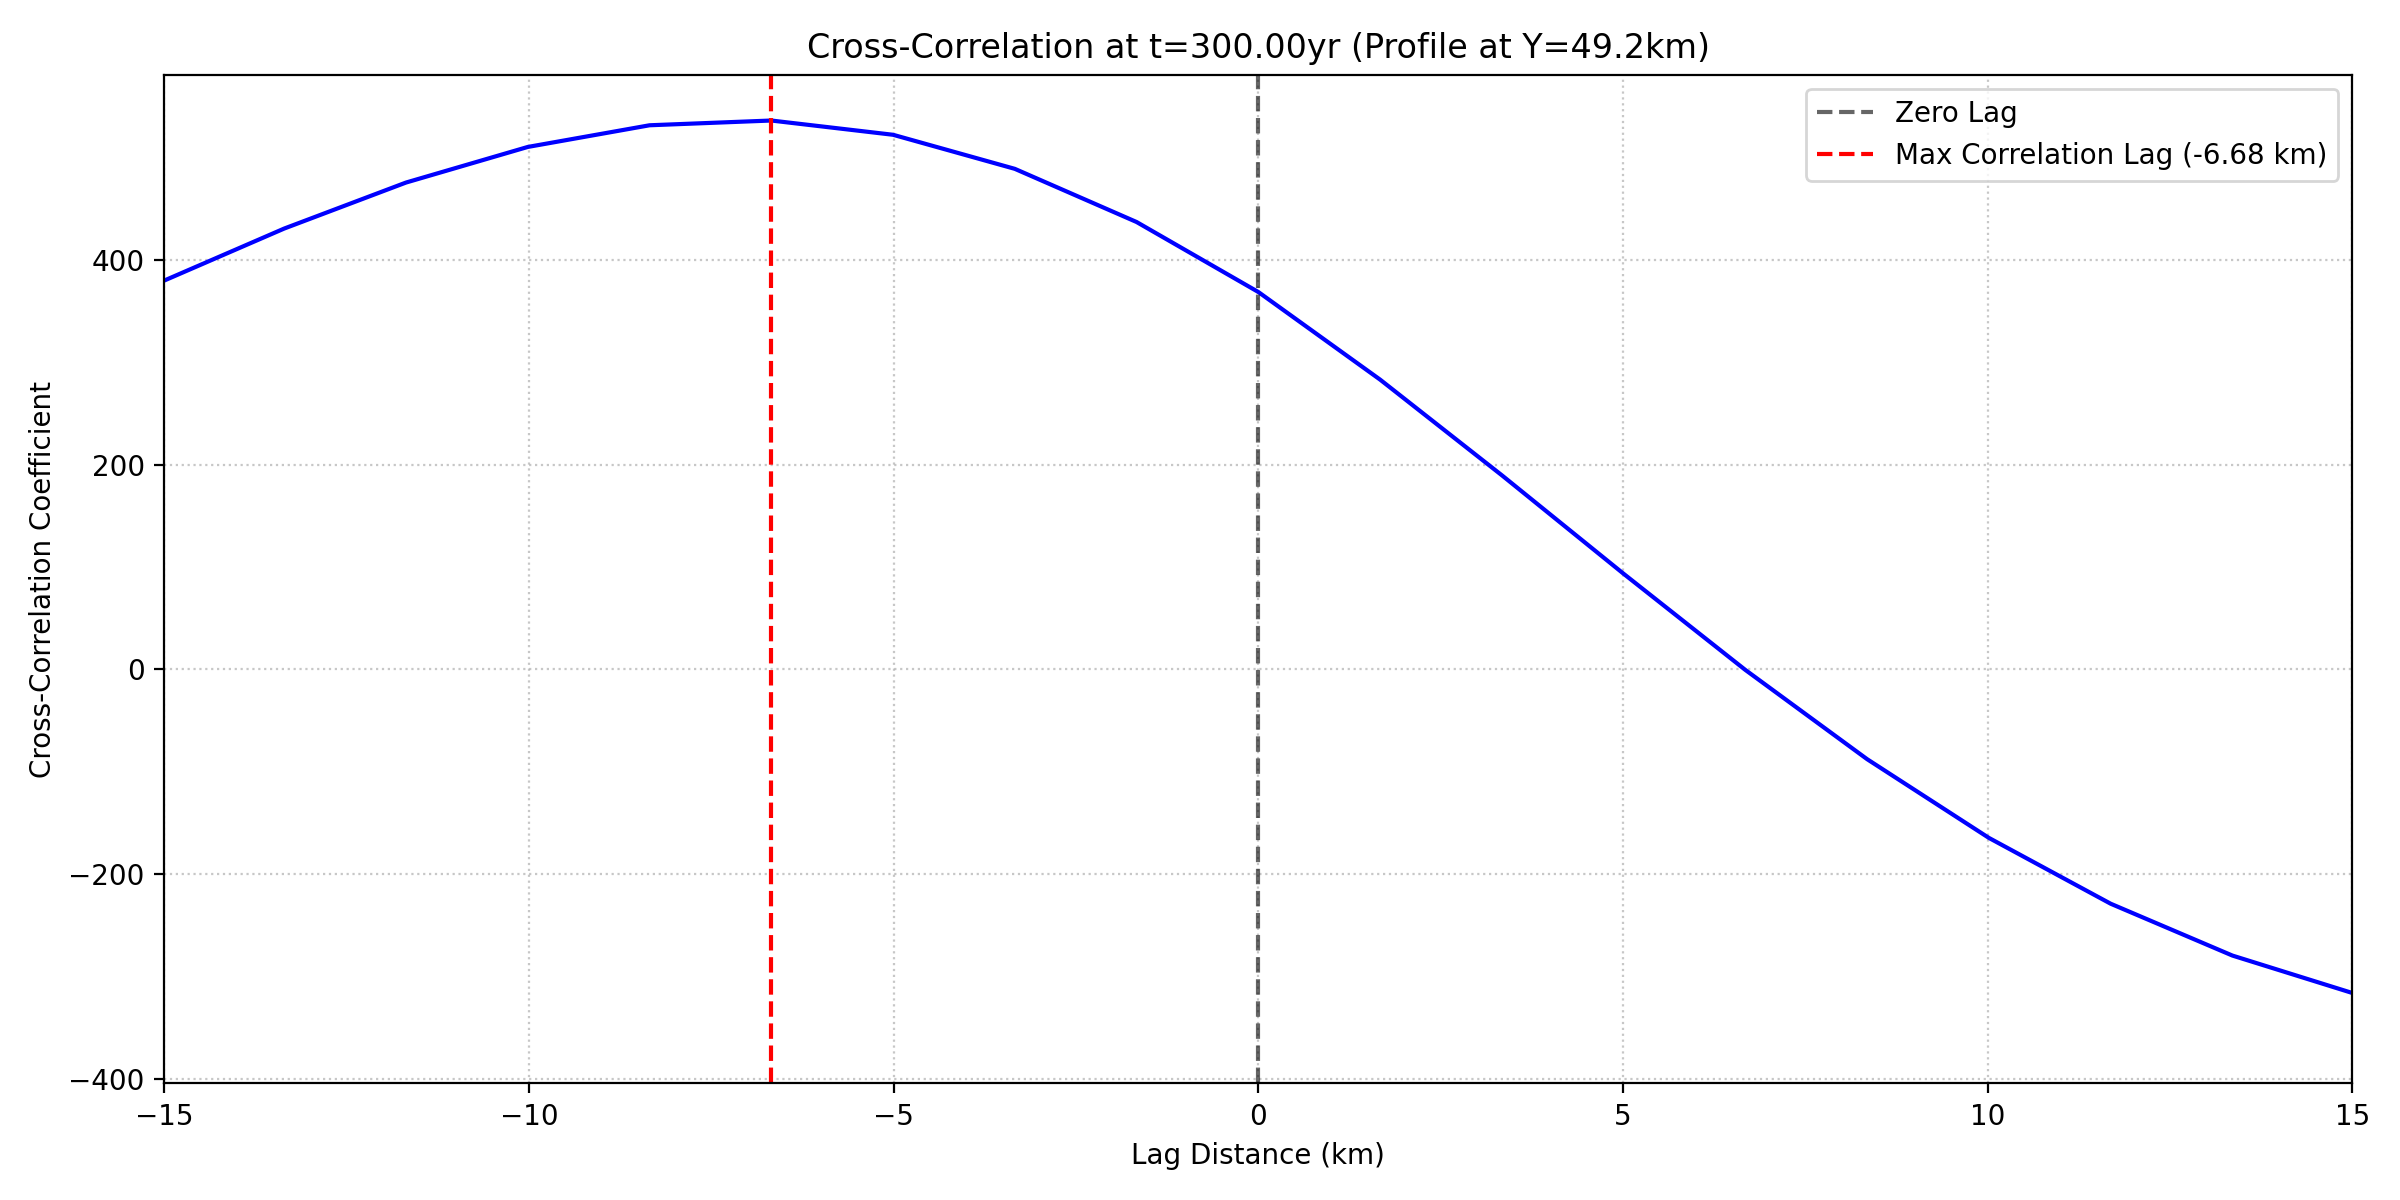
\includegraphics[scale=0.45]{figures/S2_F_correlation_t_0036.png}
%     \caption{The cross-correlation function and the detected lag of maximum correlation.}
%     \label{fig:phase_analysis_Cross_Correlation}
% \end{figure}
% \begin{figure}[H]
%     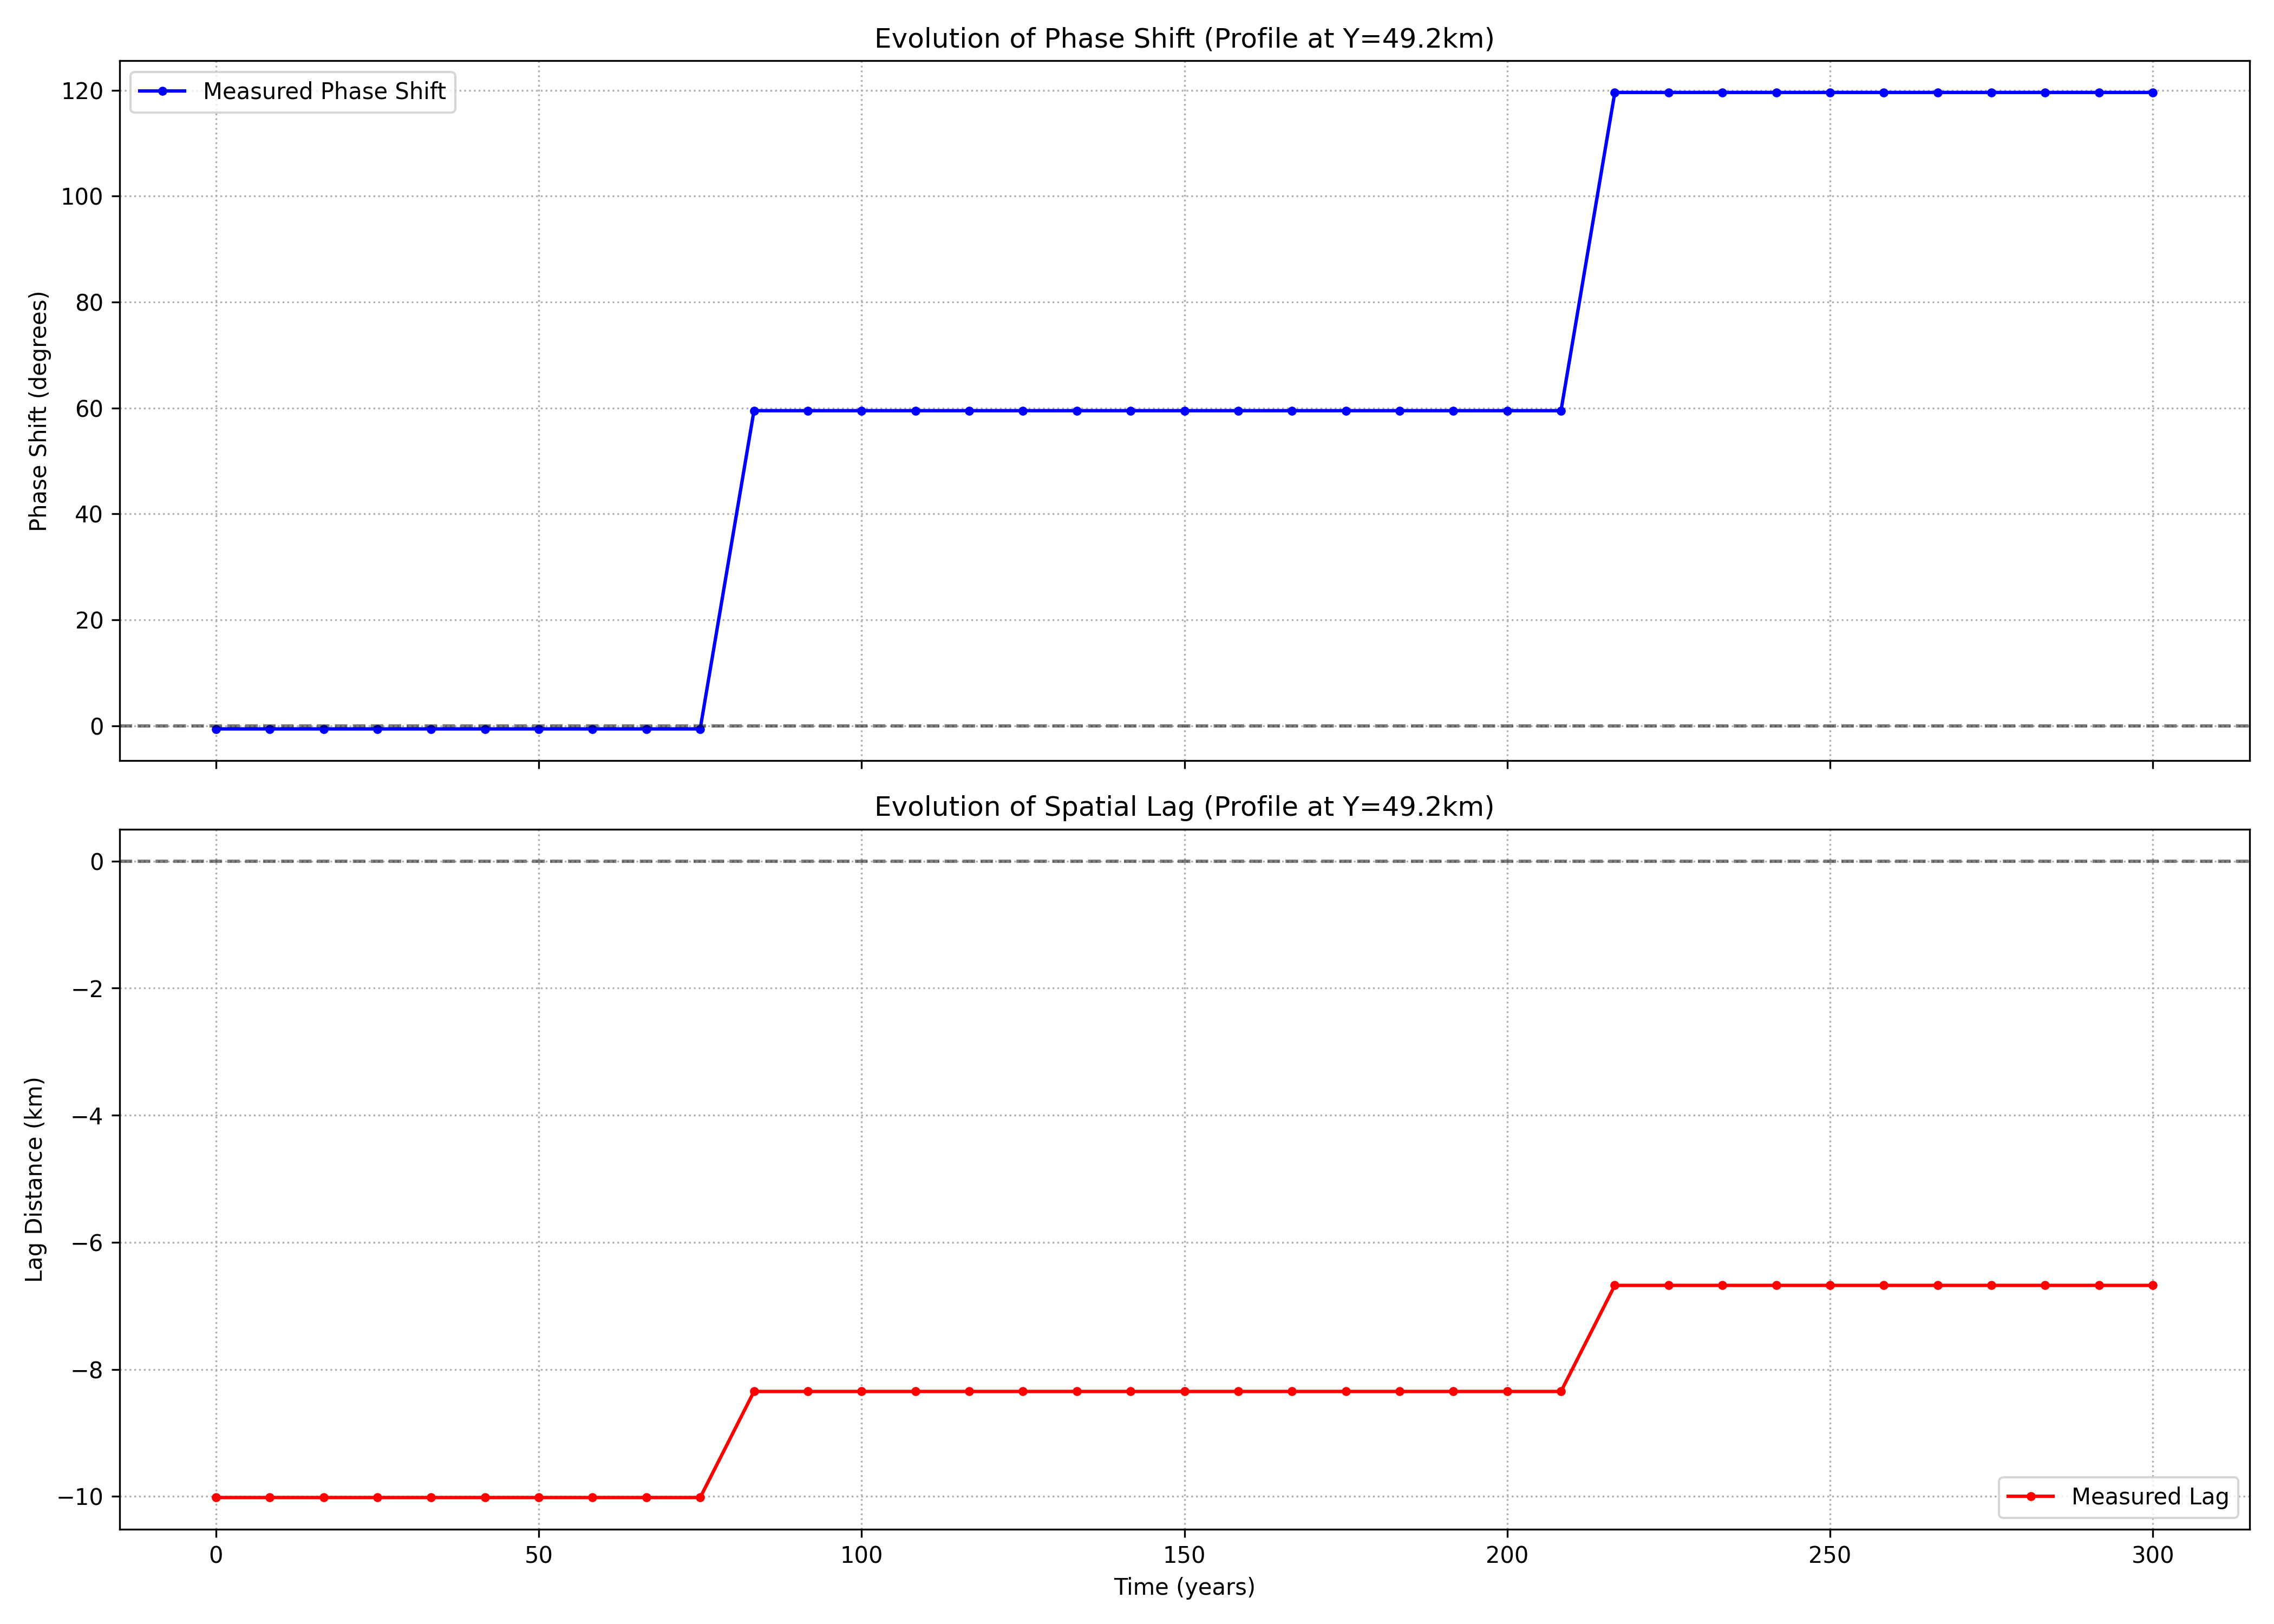
\includegraphics[scale=0.45]{figures/S2_F_phase_evolution_summary.png}
%     \caption{The evolution of the phase shift and spatial lag over the entire simulation.}
%     \label{fig:phase_analysis_Evolution_Plots}
% \end{figure}
% %%% S3
% \begin{figure}[H]
%     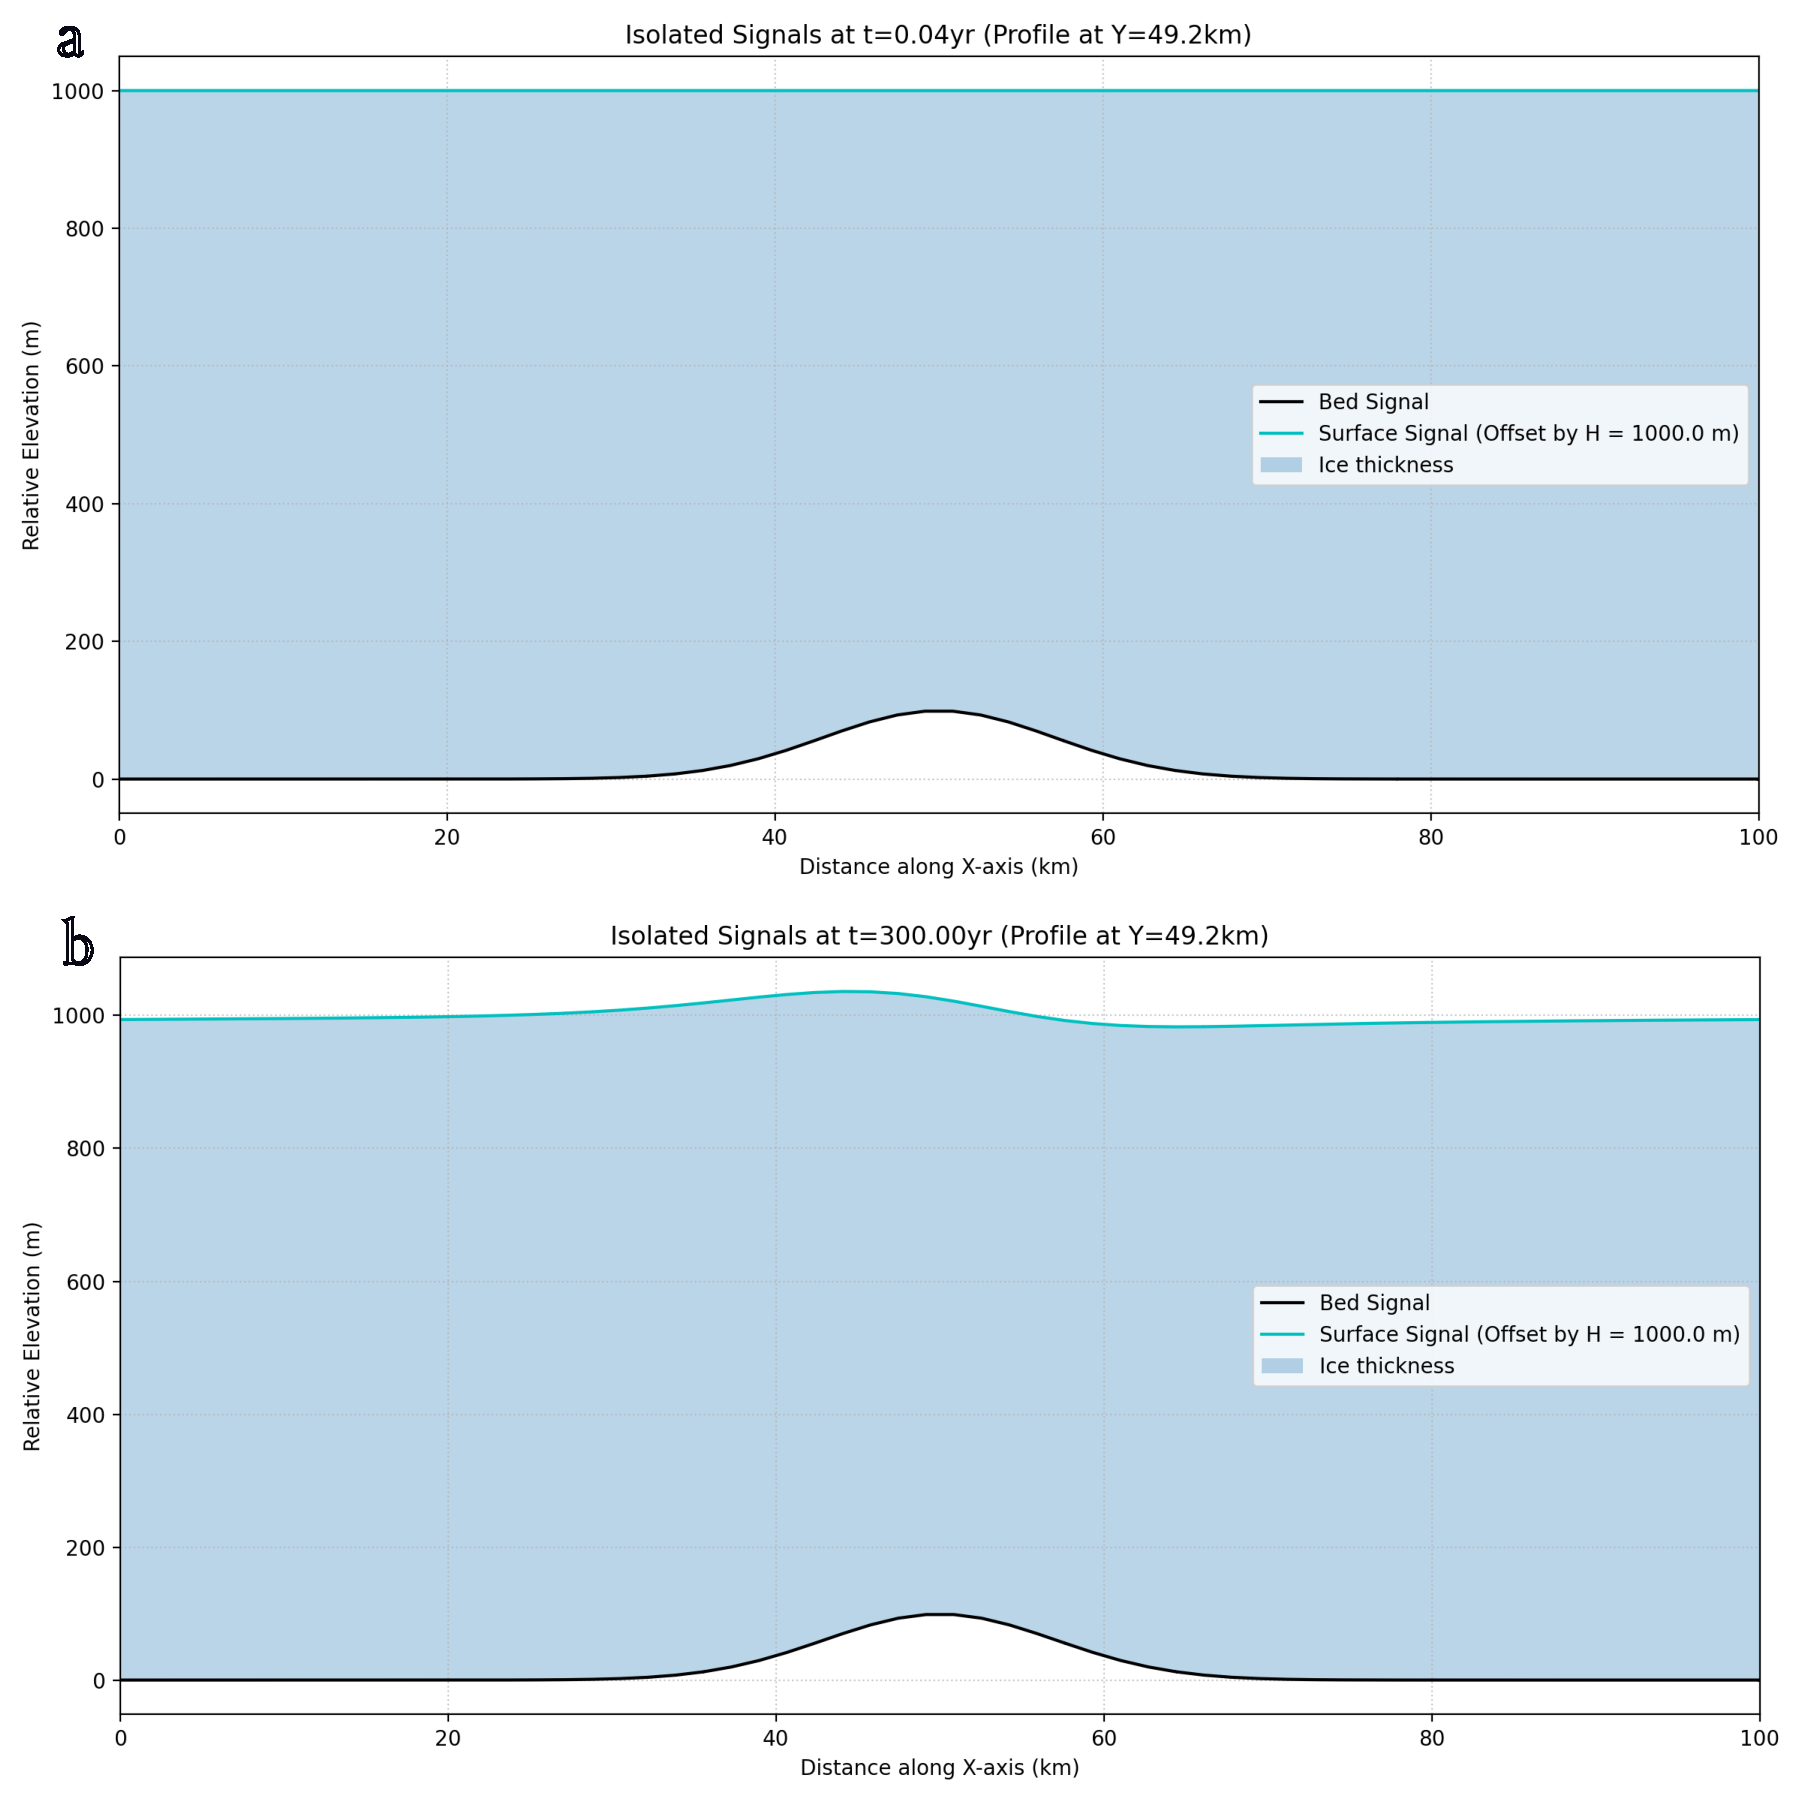
\includegraphics[scale=0.45]{figures/S3_F_signals.pdf}
%     \caption{the isolated bedrock and ice surface signals}
%     \label{fig:phase_analysis_Signals}
% \end{figure}
% \begin{figure}[H]
%     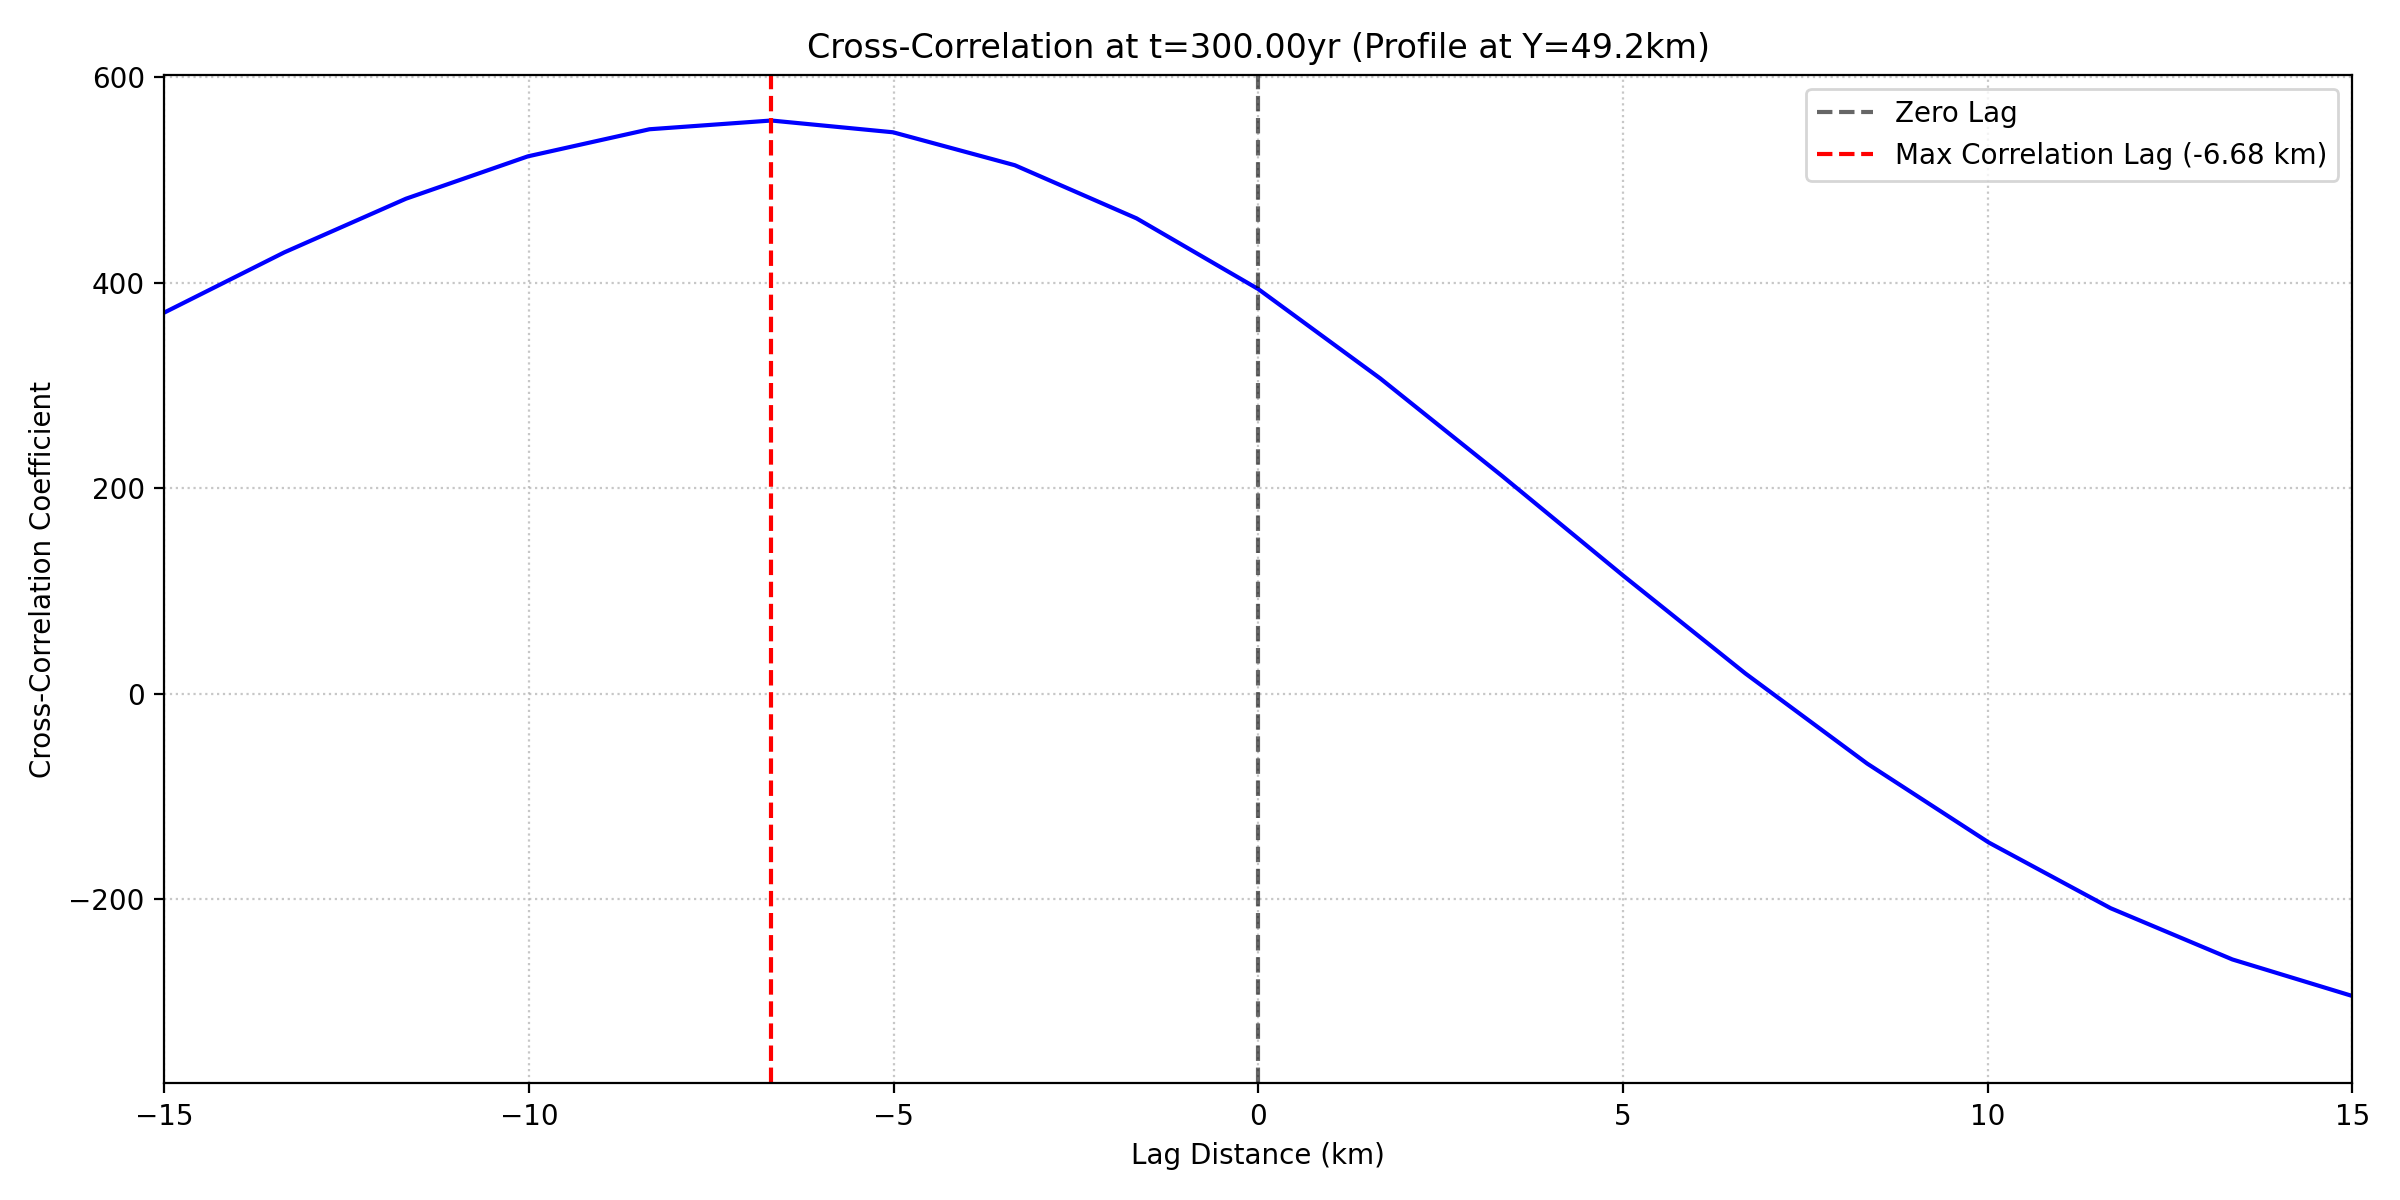
\includegraphics[scale=0.45]{figures/S3_F_correlation_t_0036.png}
%     \caption{The cross-correlation function and the detected lag of maximum correlation.}
%     \label{fig:phase_analysis_Cross_Correlation}
% \end{figure}
% \begin{figure}[H]
%     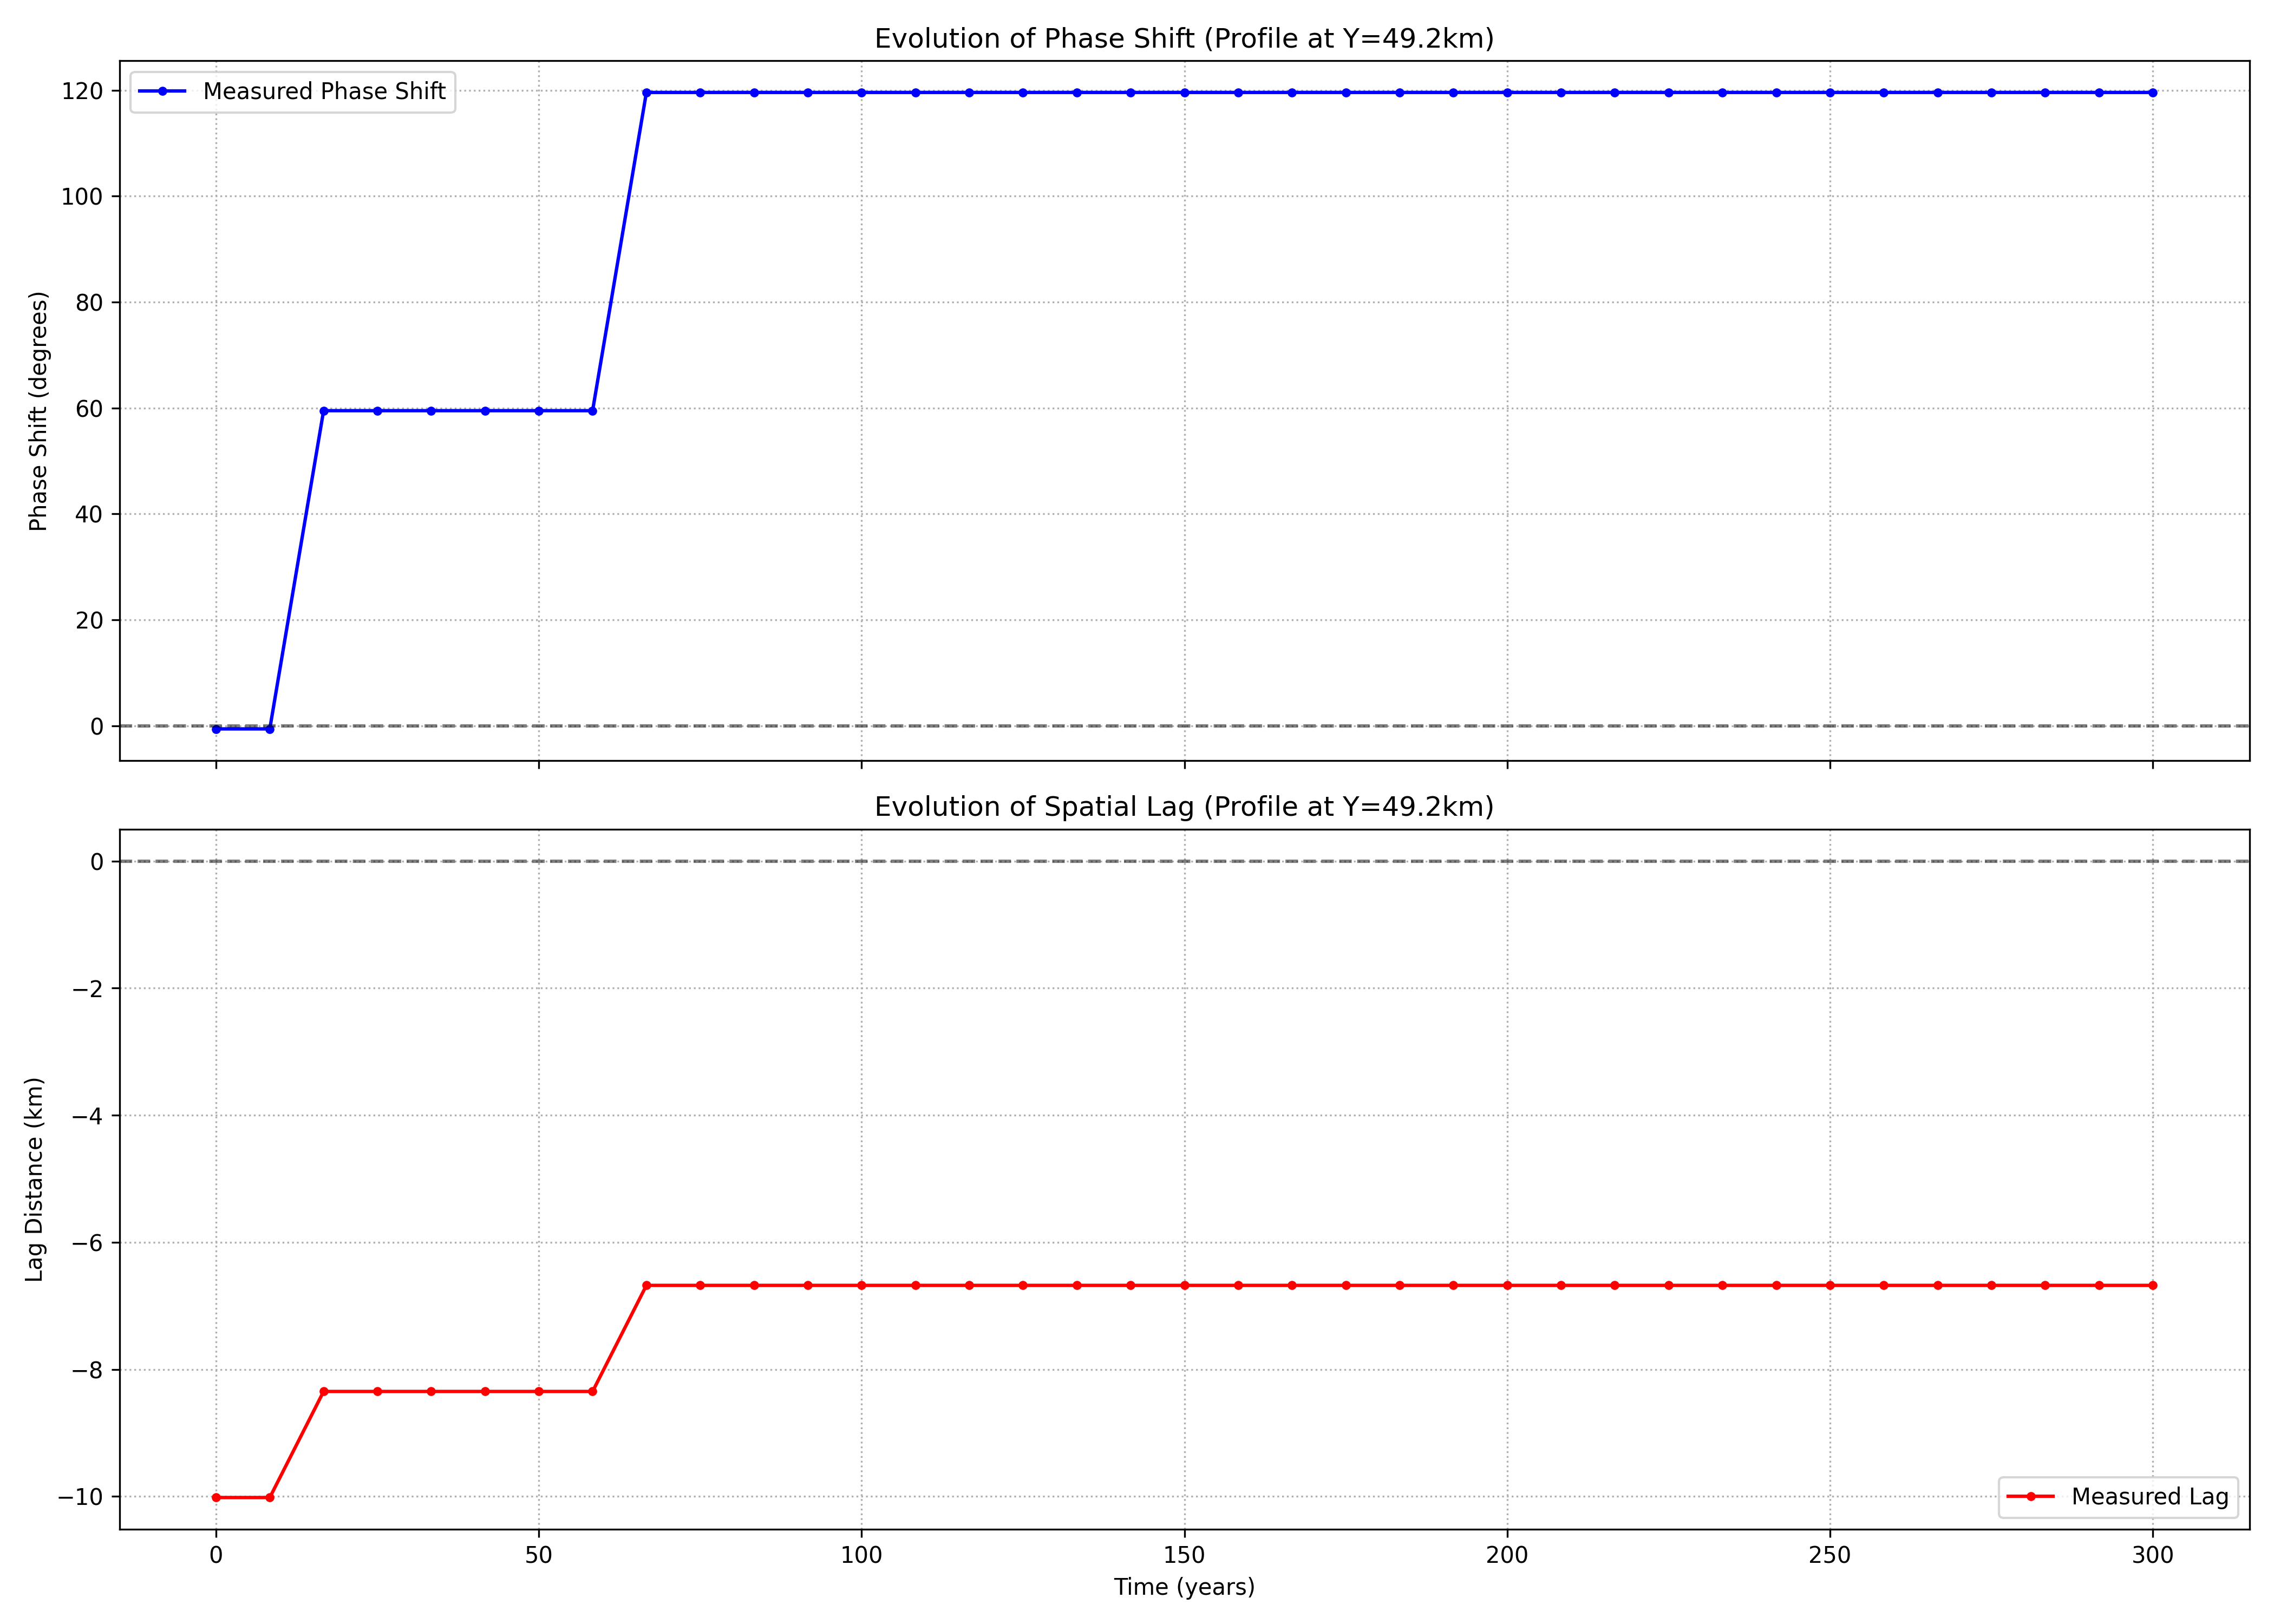
\includegraphics[scale=0.45]{figures/S3_F_phase_evolution_summary.png}
%     \caption{The evolution of the phase shift and spatial lag over the entire simulation.}
%     \label{fig:phase_analysis_Evolution_Plots}
% \end{figure}
% %%% S4
% \begin{figure}[H]
%     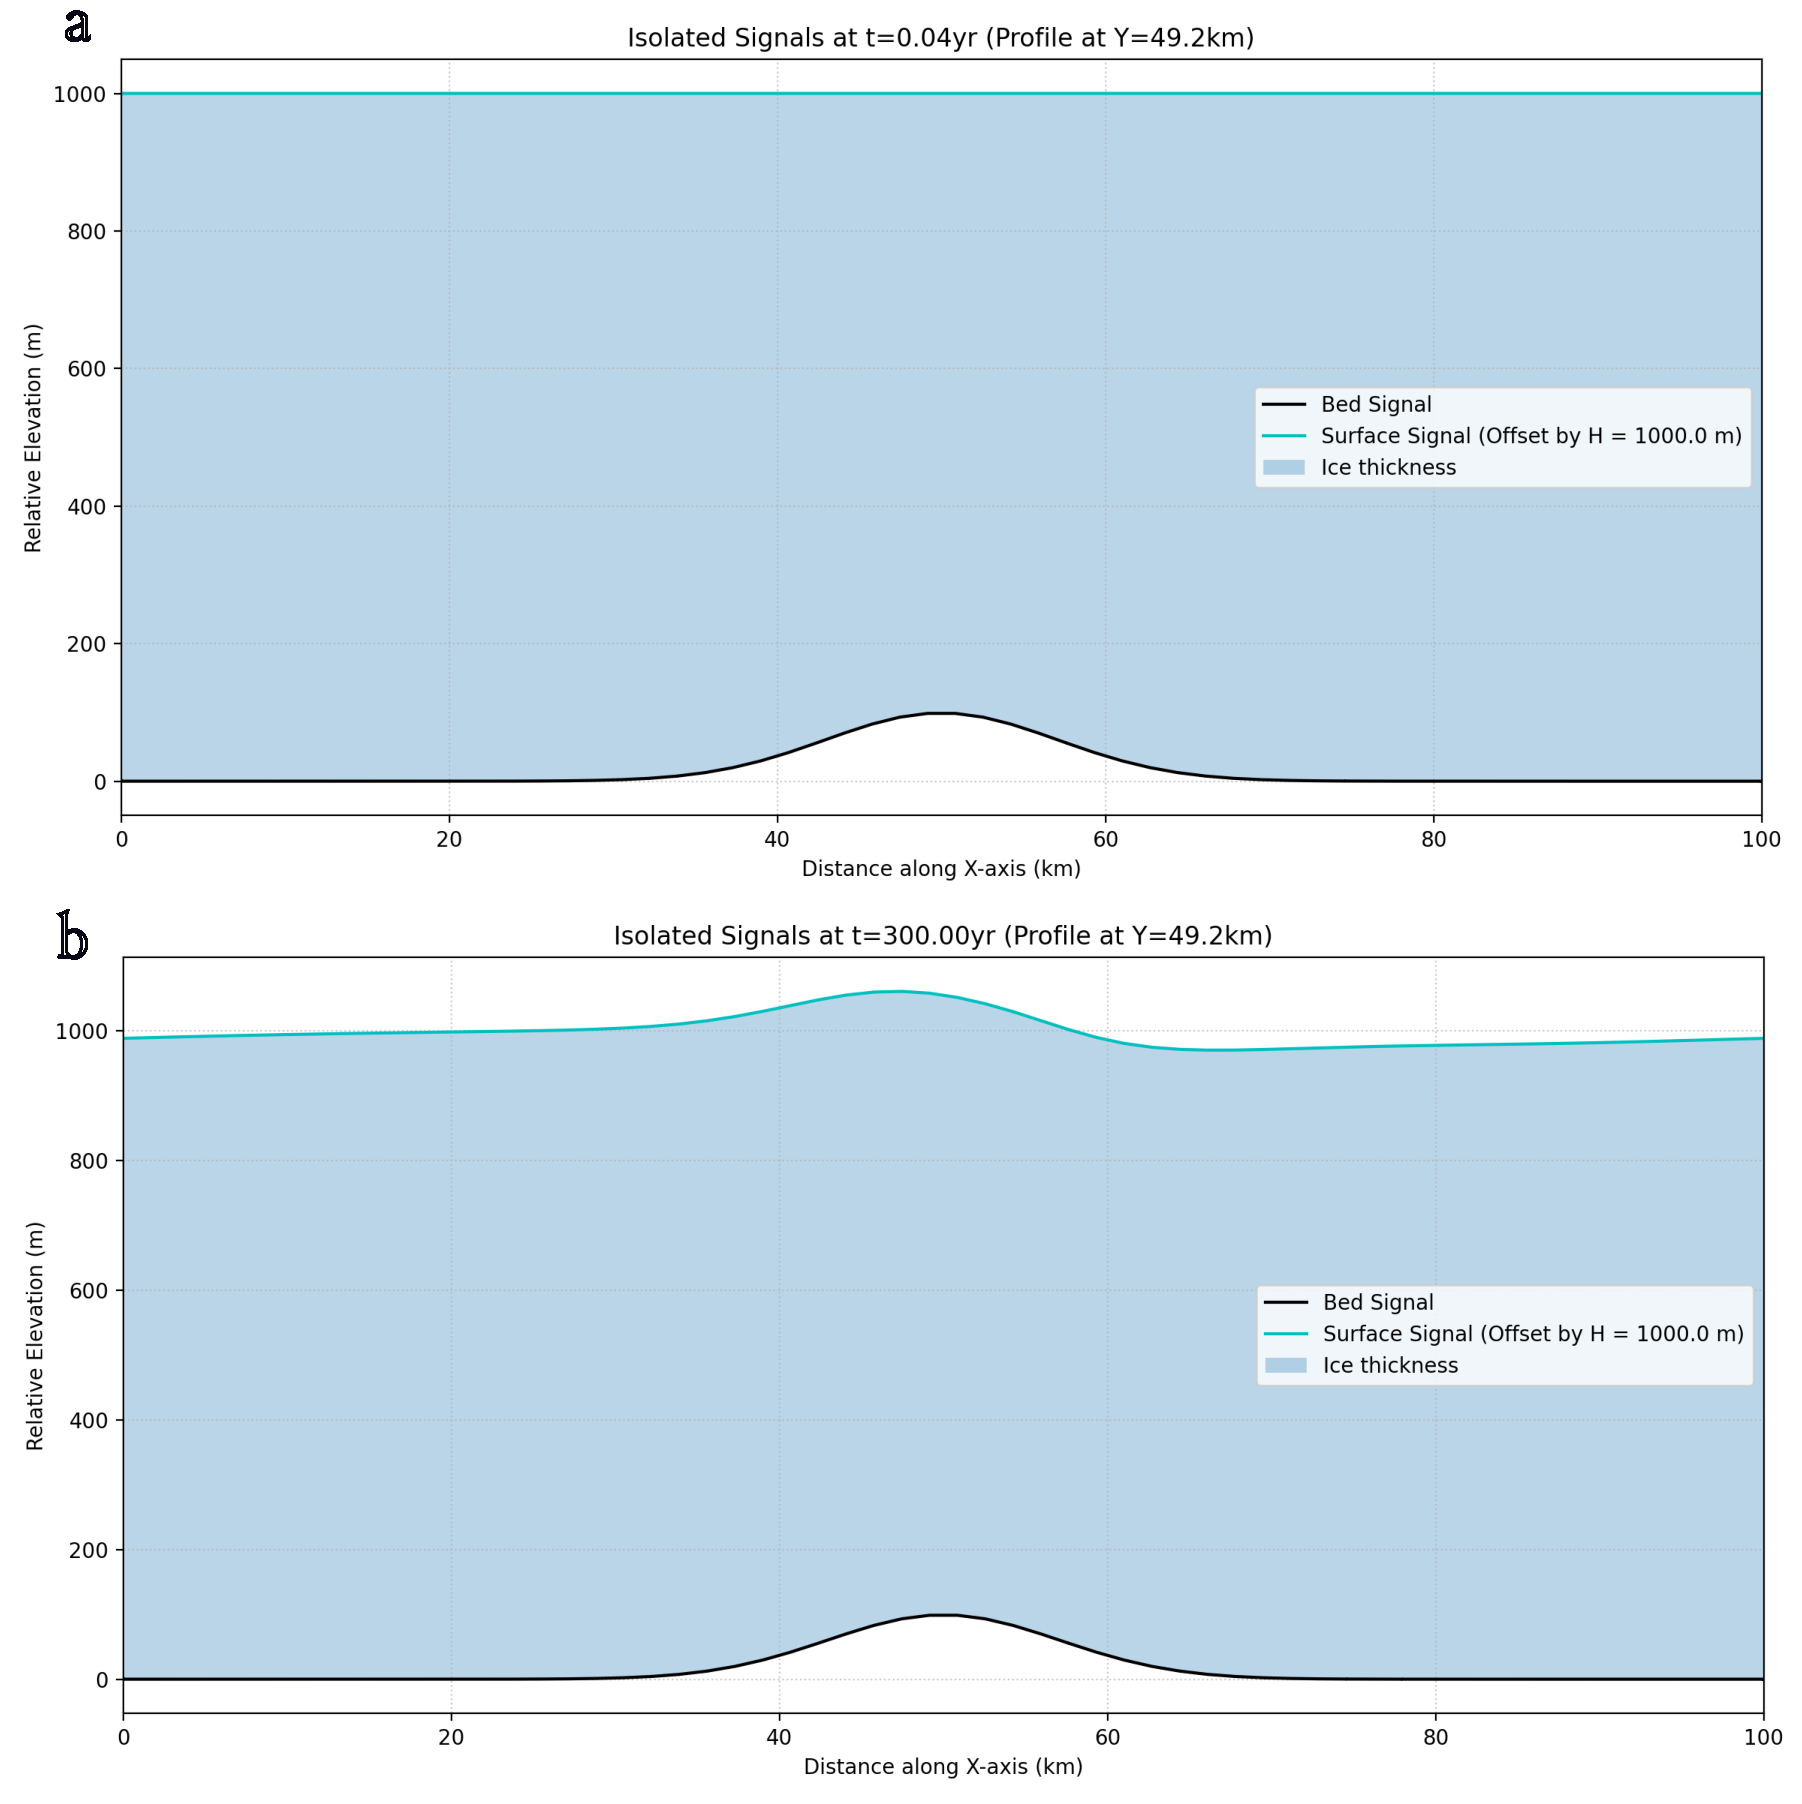
\includegraphics[scale=0.45]{figures/S4_F_signals.pdf}
%     \caption{The isolated bedrock and ice surface signals}
%     \label{fig:phase_analysis_Signals}
% \end{figure}
% \begin{figure}[H]
%     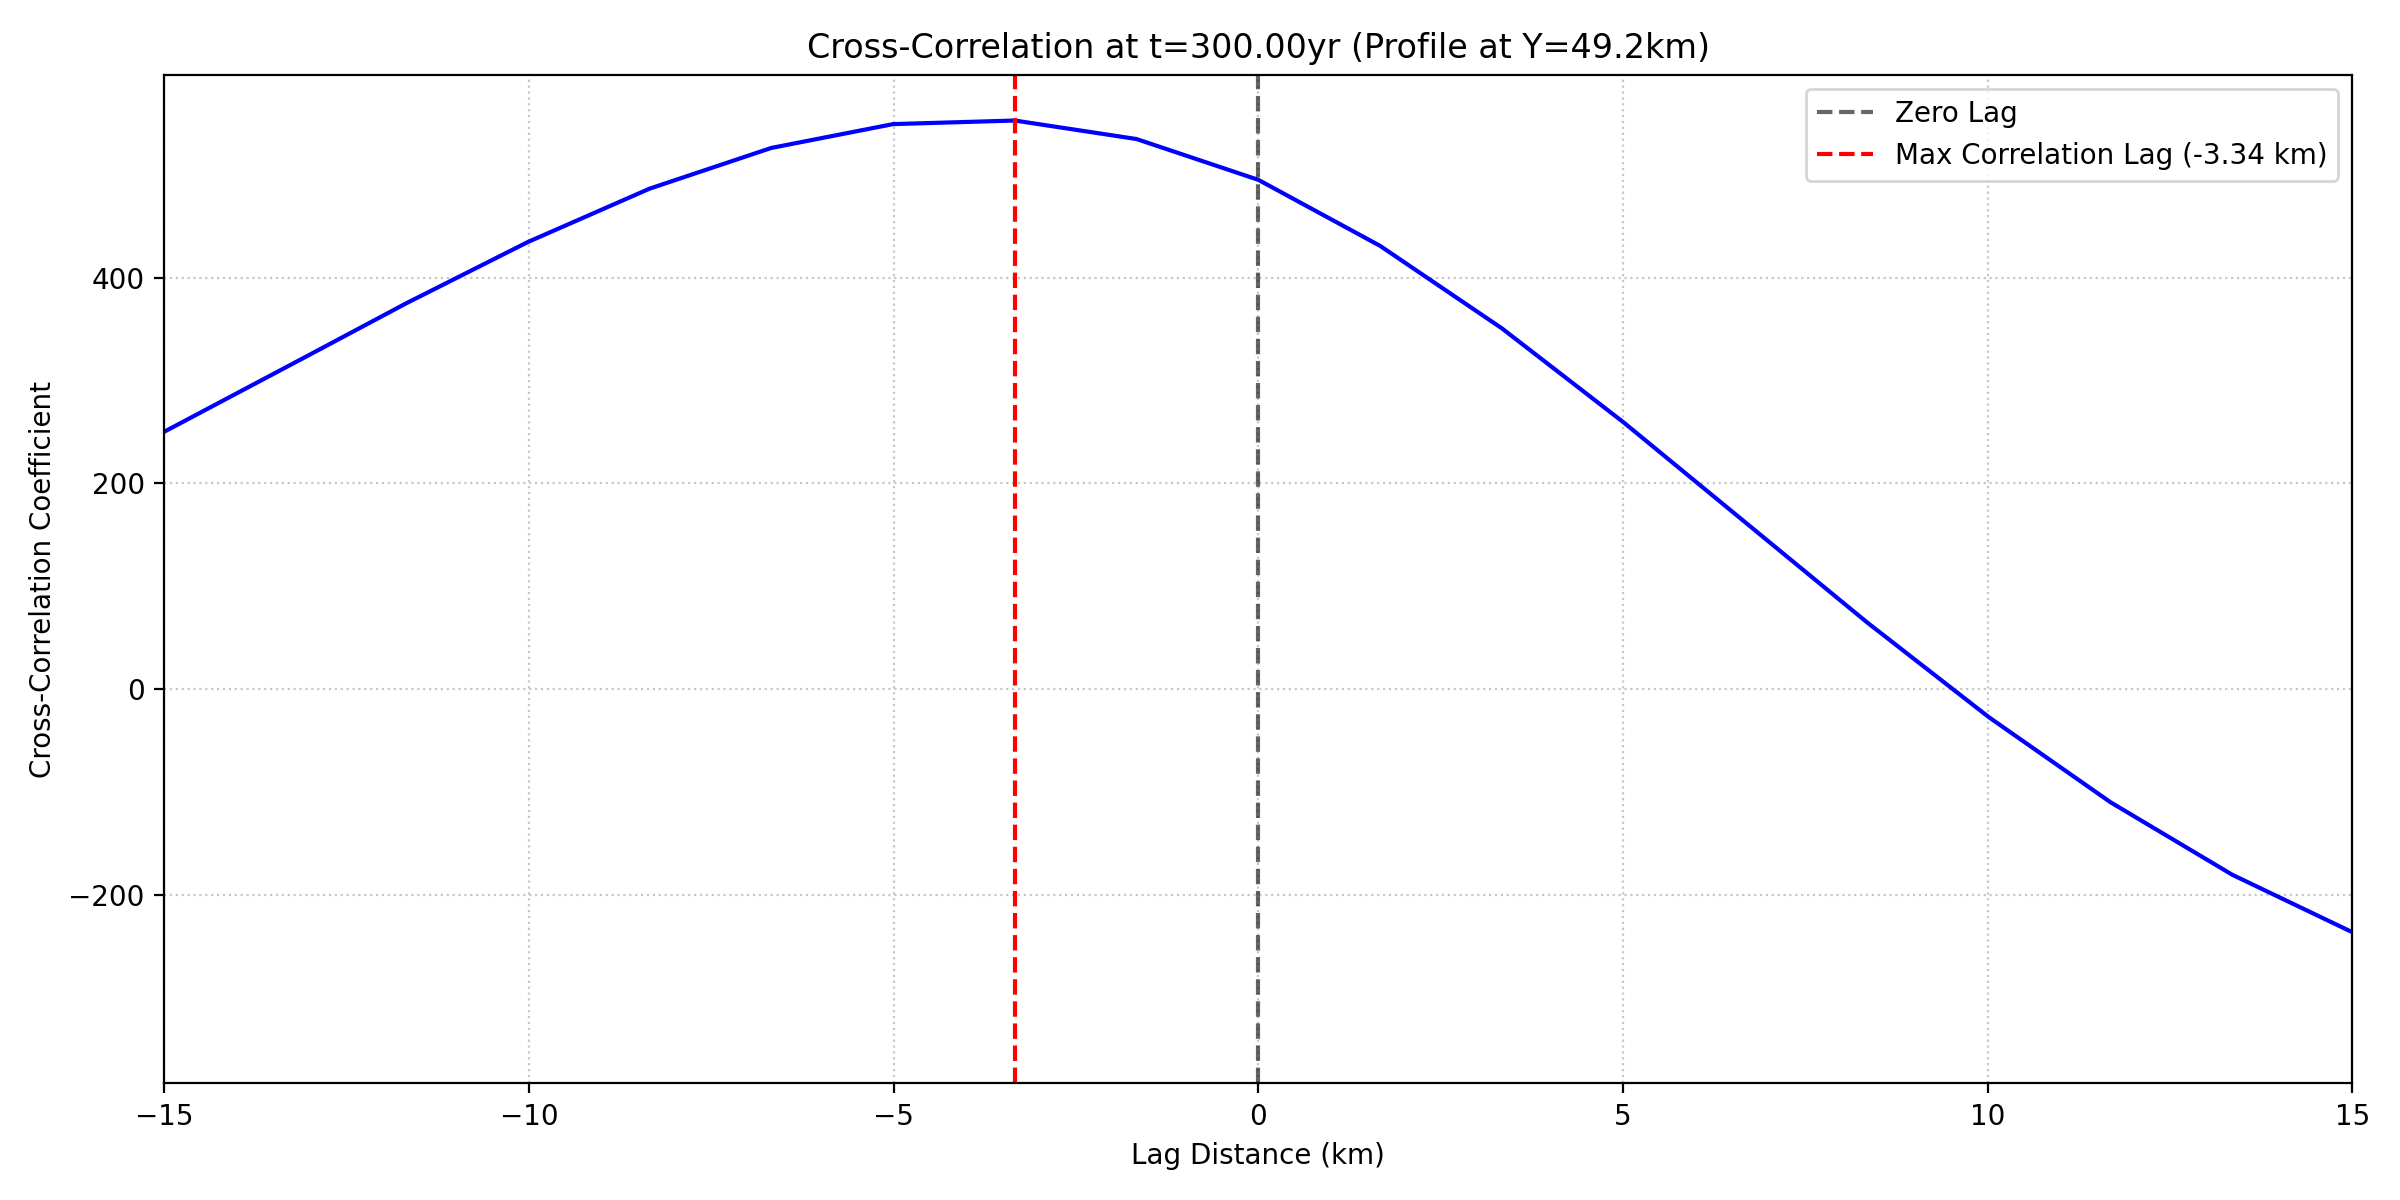
\includegraphics[scale=0.45]{figures/S4_F_correlation_t_0036.png}
%     \caption{The cross-correlation function and the detected lag of maximum correlation.}
%     \label{fig:phase_analysis_Cross_Correlation}
% \end{figure}
% \begin{figure}[H]
%     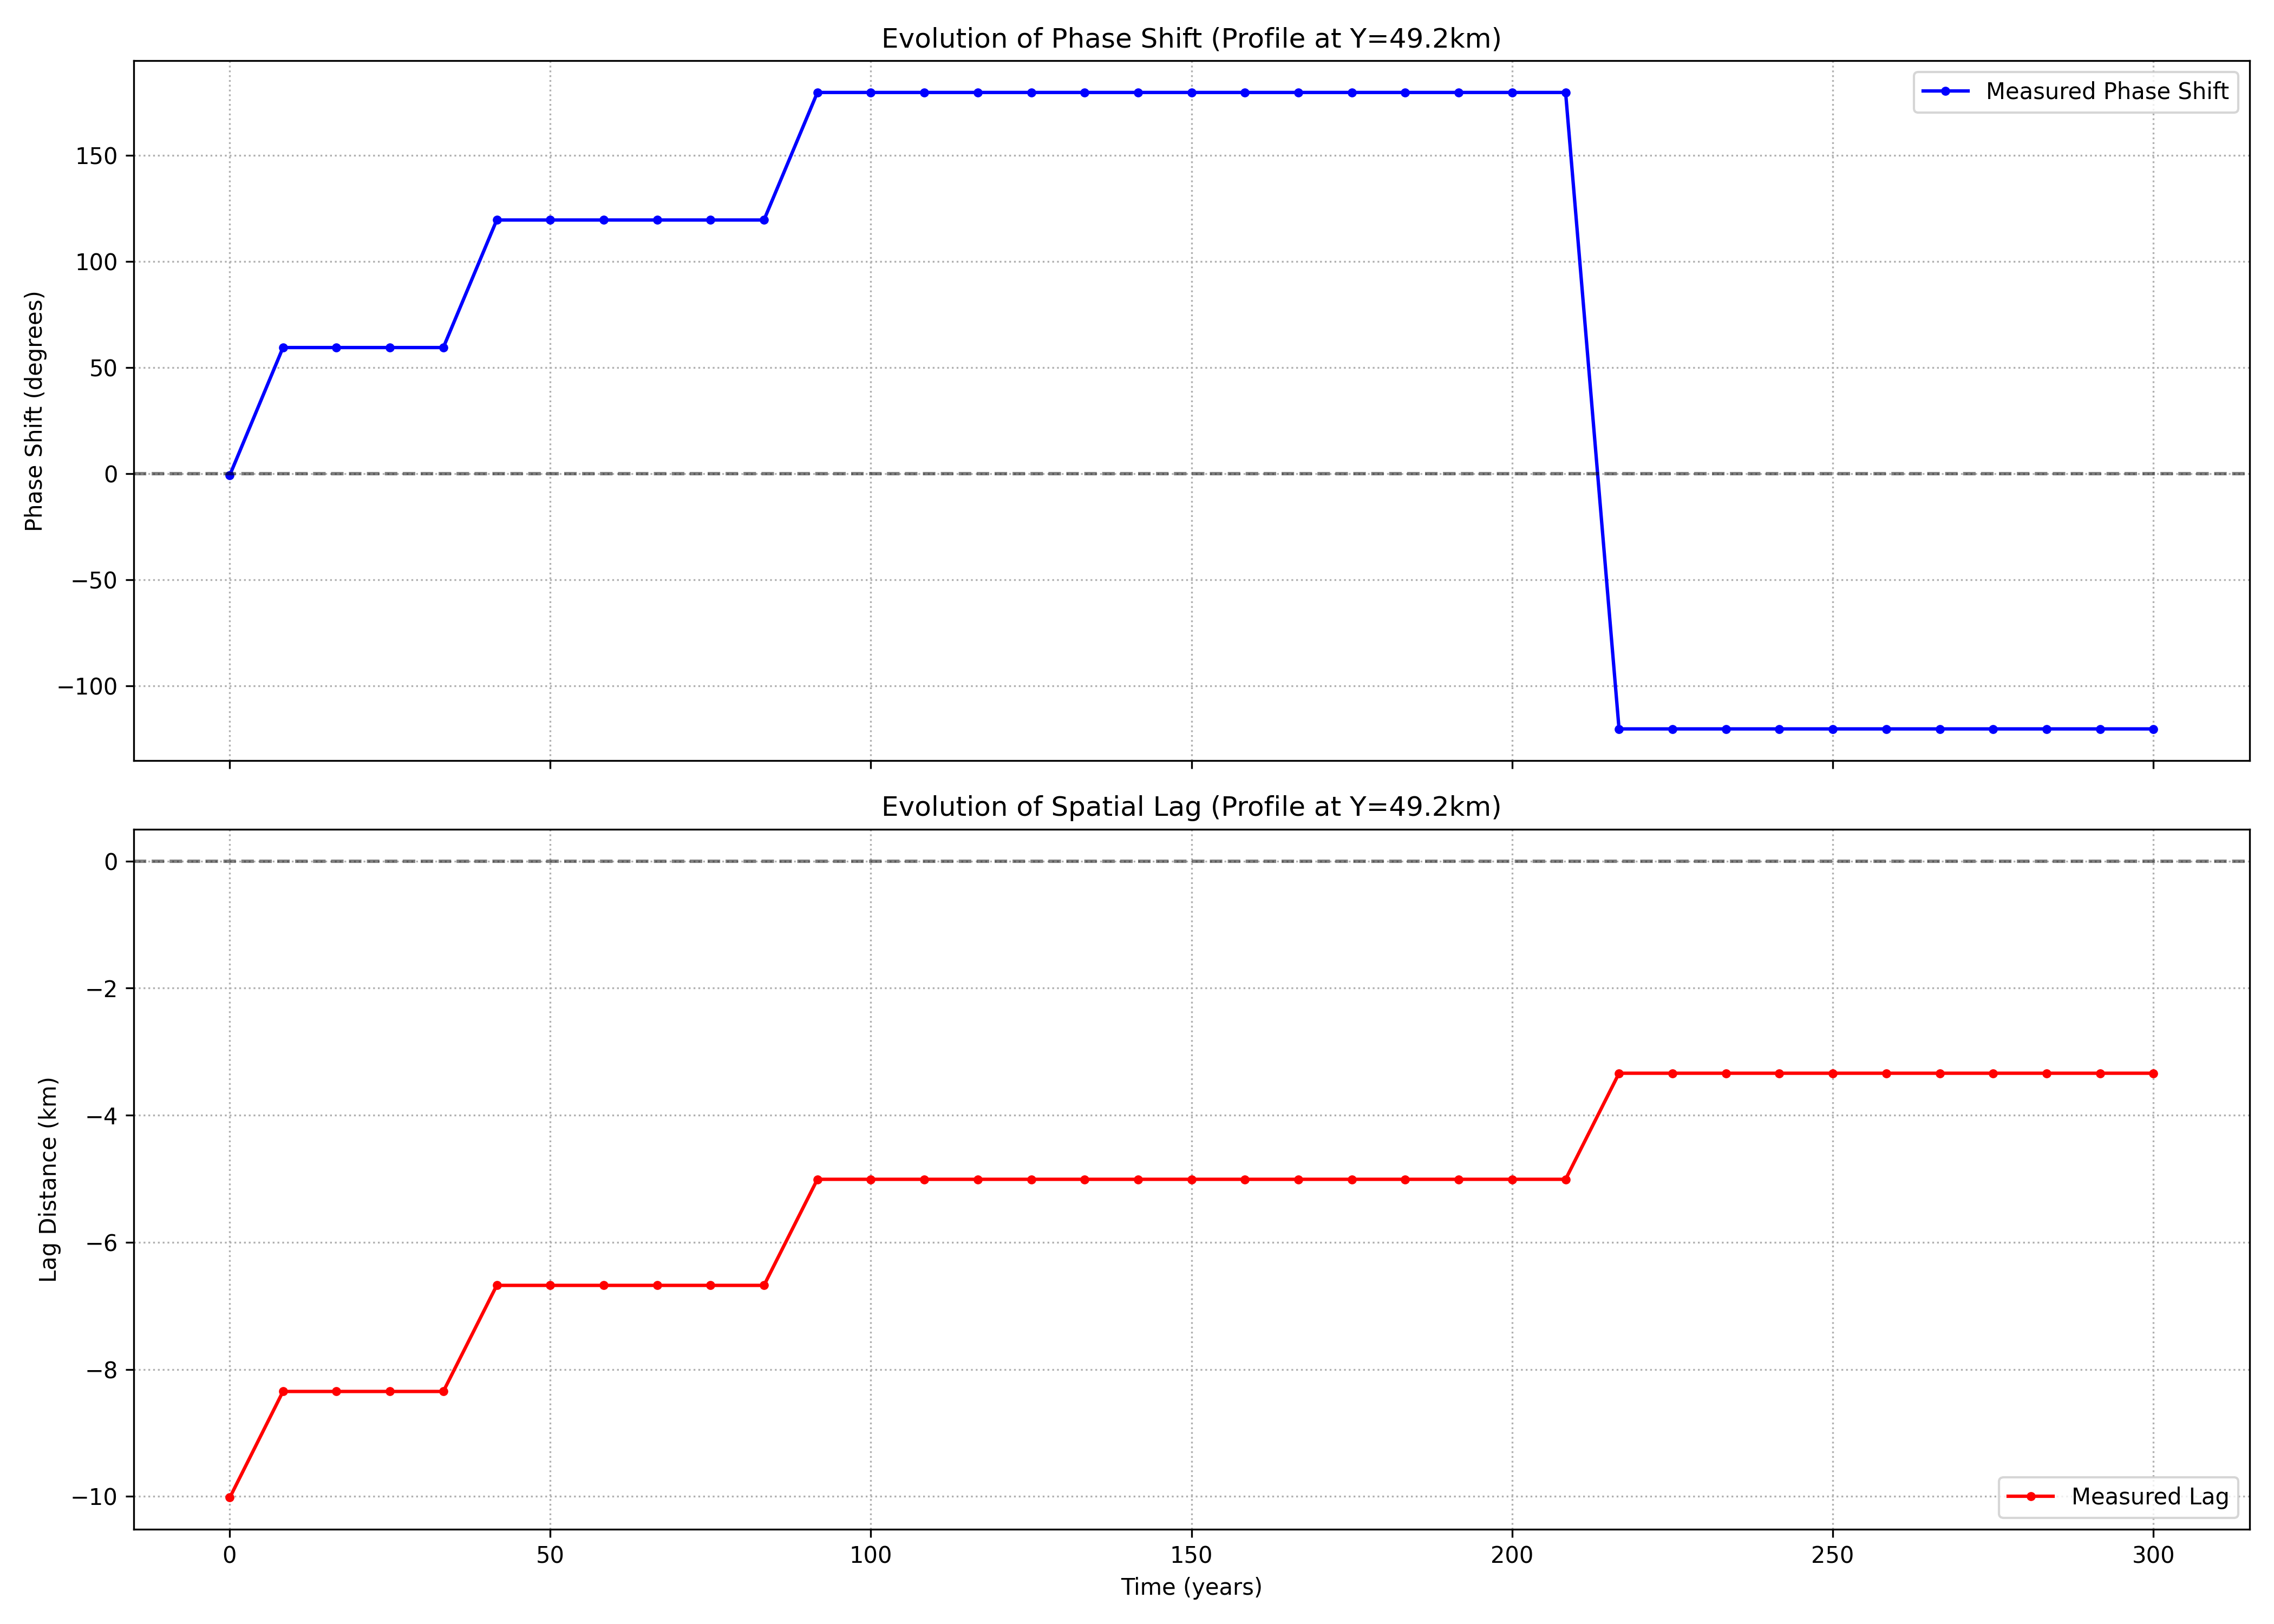
\includegraphics[scale=0.45]{figures/S4_F_phase_evolution_summary.png}
%     \caption{The evolution of the phase shift and spatial lag over the entire simulation.}
%     \label{fig:phase_analysis_Evolution_Plots}
% \end{figure}
The results for the phase analysis show that an isolated feature such as the Gaussian bump in Exp F in ISMIP-HOM produces a different phase shift ($\approx~\frac{2\pi}{3}$). This results highlights the limitations of applying Budd periodic theory to non-periodic features.

\section{Current Conclusions}

% % ======================================================

% \subsubsection{Transient Analysis}
% % \begin{figure}[H]
% %     \includegraphics[scale=0.45]{figures/}
% %     \caption{}
% %     \label{fig:Transient_analysis}
% % \end{figure}
